\documentclass[12pt,a4paper]{scrreprt}
\usepackage[utf8]{inputenc}
\usepackage[main=german,provide=*]{babel}
\usepackage[T1]{fontenc}
\usepackage{graphicx}
\usepackage{hyperref}
\usepackage[automark,headsepline,plainheadsepline]{scrlayer-scrpage}
\usepackage{listings} 
\usepackage[backend=biber, url=true, sorting=none]{biblatex}
\usepackage{csquotes}
\usepackage{wrapfig}
\usepackage[left=2cm,right=2cm,top=2cm,bottom=2cm]{geometry}

\defbibheading{lit}{\section{Literaturverzeichnis}}
\defbibheading{on}{\section{Onlineverzeichnis}}
\defbibheading{vor}{\section{Vorträge und Predigten}}
\addbibresource{Quellenverzeichnis.bib}
\hypersetup{
colorlinks=true,
linkcolor=black,
urlcolor=black,
citecolor=black,
}
\setlength{\parindent}{0pt}
\graphicspath{{Bilder/}}
\automark[section]{chapter} 
\clearpairofpagestyles
\ihead{\leftmark}
\ohead[\thepage]{\thepage}


\author{Felix Brugger}
\title{Mein Credo --- Ein Versuch, meinen Glauben zu beweisen}
\date{6. Februar 2015}

\setcounter{secnumdepth}{5}
\setcounter{tocdepth}{5}

\begin{document}
\pagestyle{empty}
\begin{figure}[h]
    \begin{center}
        
\includegraphics[width=\linewidth]{Kreuz}
    \end{center}
\end{figure}

\bigskip
\bigskip
\bigskip

\begin{center}
    \Huge{\textbf{Mein Credo}}
    \linebreak
    \bigskip
    \large{Ein Versuch, meinen Glauben zu beweisen}
\end{center}

\newpage
\pagestyle{scrheadings}
\tableofcontents
\newpage

% !TEX root = Mein Credo.tex
\part{Vorwort}
\chapter*{Vorwort}
Seit meiner Geburt wuchs ich nach protestantischen Glauben auf, nahm dessen Werte an, sog dessen Inhalt auf und spätestens ab meinen 13. Lebensjahr war mein Glauben ein essentieller Bestandteil meines Lebens.
\\~\\
Wie jeder Mensch entwickelte ich mich. Mein Leben war eine Achterbahnfahrt. Als Kind sog ich die Inhalte des Glaubens in mich auf. Es war nur ein oberflächliches ankratzen der wirklich wichtigen Sachverhalte, doch ich war begeistert. Da ich nicht getauft war, hab ich darauf bestanden, getauft zu werden. Nach langen bearbeiten meiner Mutter wurde ich am 1. Juli 2007 getauft. Ich dachte, dass nichts und niemand in meinen Leben meinen glauben im Weg stehen könnte. Doch es kam eine  Zeit der persönlichen Herausforderungen. Im Angesicht diesen Herausforderungen konnte ich immer weniger an Gott glauben. Auch mithilfe meines Glaubens bezwang ich jedoch diese Situationen. Der Glauben prägte mein Leben und ließ gewisse Werte in mich einbrennen.
\\~\\
Über die Jahre zweifelte ich wie jeder gute Christ an meinen Glauben und begann die Sachverhalte zu hinterfragen. Da ich auch (natur-) wissenschaftlich veranlagt bin  -wahrscheinlich habe ich das durch meinen Vater geerbt- wollte ich meinen Glauben wissenschaftlich und theologisch hinterfragen. In meinen 17. Lebensjahr entschied ich mich, meinen Glauben von Grund auf kritisch zu hinterfragen und daraus mein Credo zu ziehen. Mit dem Gedanken im Hinterkopf, dass dies hier subjektiv geprägt sein wird und es kein absolutes, rationales Ergebnis bei einen irrationalen Thema möglich ist, beginne ich, meine komplizierten Denkvorgänge, Folgerungen, Schlüsse, Ansätze u.v.m.\ u.v.m. hier zu verschriftlichen mit dem Ziel, meinen eigenen Credo aufzustellen und hier festzuhalten, woran ich Glaube.
\\~\\
Egal ob mein Credo zu einen zufriedenstellenden Ergebnis kommt oder nicht, egal ob ich in ferner Zukunft immer noch der Kirche angehöre oder nicht, ich bereue meinen Glauben nicht. Ich bin mir sicher, dass die Erfahrungen und Werte, die mich geprägt haben, in jeder Weise im Leben weiterhelfen werden. Als Dokumentation halte ich hier nun alles für mich und meine Nachwelt schriftlich fest. Entschuldigen sie meine eher merkwürdige Sprache und meine für sie Wirr erscheinenden Gedankengänge. Dieses riesige Projekt wird mich hoffentlich eine sehr lange Zeit begleiten und hoffentlich zu einen Ende kommen. Wenn nicht, dann ist es so. Wenn ja, dann spiegelt dieses Stück nicht nur meinen Credo wieder, sondern ein Stück meines Lebens.
\\~\\
Nun stehe ich hier, bereit anzufangen. Vielleicht bin ich einfach nur verrückt. Vielleicht werde ich in ein paar Jahren nur schmunzelnd dies hier lesen und mich über meine eigene Naivität auslachen. Aber es ist mir egal. Ich habe mich immer wie ein verrückter Volldepp aufgeführt und es hat mich nie im Ansatz gejuckt.  Also starte ich dieses Projekt ohne den Gedanken, was andere hierüber denken können oder kurz gesagt: Es juckt mich nicht, was andere hierüber denken.
\newpage
Zum Projekt: Dies ist eine sehr, sehr stark zusammengefasste Version meines Wissens. Für mich wichtige Stellen werden ausführlicher erläutert und eher unbedeutende oder leicht zu erklärende Stellen stark komprimiert. Die hierfür herangezogenen Quellen werden kritisch hinterfragt und zusammengetragen, jedoch nicht wissenschaftlich korrekt zitiert. Einige Stellen werden eine einzige Redaktion vieler Quellen sein und ich werde einen Teufel tun, jede einzelne Quelle an den entsprechenden Stellen zu zitieren, da der Aufwand dafür zu groß wäre. Diese Arbeit dient ganz und allein mir und Gott und wir pfeifen auf banale Formalitäten. Die Quellen werden am Ende aufgeführt und es steht jeden frei, die Quellen zu überprüfen. Dies ist mein Credo und keine wissenschaftliche Thesis. Formalitäten spielen hier eine untergeordnete Rolle. Umso mehr spielt der Inhalt eine Rolle. Und der ließt sich besser ohne 3 Milliarden Quellenverweise.
\bigskip
\begin{flushright}
\textit{Aichwald, den \today}
\end{flushright}
\bigskip
\bigskip
\bigskip
\bigskip
\bigskip
\bigskip
\bigskip
\bigskip
\bigskip
\begin{figure}[h]
\begin{flushright}

\includegraphics[scale=0.7]{Signatur.jpg}\\
$\overline{~~~~~~~~~\mbox{Felix Brugger}~~~~~~~~~}$
\end{flushright}
\end{figure}

% !TEX root = Mein Credo.tex
\part{Die Theologie als Wissenschaft}
\chapter{Das Problem der Theologie als Wissenschaft}
Die heutige Theologie ist schwierig zu den konventionellen Wissenschaften einzuordnen. Die Theologen sind keine reine Philosophen, sie sind keine reinen Historiker, sie sind keine reine Sprachwissenschaftler und sie sind keine reinen Ethiker. Doch alles spielt in die Theologie mit rein. Es steht außer Frage, dass die Theologie mit wissenschaftlichen Kriterien und Methoden arbeitet. Und in der Konkurrenz der anderen, großen Geisteswissenschaften muss sie das auch, um sich den Titel der Wissenschaft zu verdienen. Dennoch setzt sich die Theologie mit etwas übernatürlichen auseinander, dass weder wissenschaftlich bewiesen noch widerlegt werden kann. Sie kann genauso wie die Historik mit Fakten arbeiten, die durch z.B. archäologischen Funde belegt werden können. Doch schlussendlich stoßt sie an eine Punkt, der außerhalb der Fähigkeiten einer Wissenschaft liegt. Einen Punkt, indem es nur noch Glauben gibt oder nicht Glauben. Dennoch wird versucht, solche irrationale Gegebenheiten mit rationalen Kriterien und Methoden zu erklären. Die Theologie versucht immer mehr, aus dem Glauben Wissen zu machen und dies ist unmöglich.
\\ 
Die Konsequenz ist, dass Theologen sich immer mehr als Wissenschaftler sehen. Der Glaube an Gott ist sporadisch vorhanden, jedoch gleicht die innere Einstellung mehr die eines Agnostikers. Theologen sind bei ihren Exegesen kritisch eingestellt. Sie wollen eher Gottes Botschaft kritisieren, anstatt diese gründlich zu erschließen. Irrationales wie Prophetie wird versucht zu falsifizieren und Rationales zu verifizieren. 
\\ ~ \\
Ein Beispiel für diese Entwicklung ist die historisch-kritische Forschung. Diese Methodik wird seit dem 20 Jh. angewandt und arbeitet mit rationalen Maßstäben. Nach 60 Jahre historisch-kritischer Forschung stellt sich die Frage, welchen Nutzen die sie für den Glaubenden gebracht hat. Die Antwort ist, dass es kaum einen gab. Wir können zwar den Entstehungsprozess einiger Bücher rekonstruieren, jedoch sind die Rekonstruktionen teilweise sehr umstritten. Sie sucht nie einen Weg, die Ergebnisse stimmig in den Glauben einzufügen. Die Ergebnisse müssen sich nicht in den Glauben einfügen, sonder der Glaube muss sich in den Ergebnissen einfügen. Die historisch-kritische Methode hat systematisch den Glauben zerlegt. Doch das Problem ist nicht die Methode an sich, sondern das Ziel der Anwender. 
\\ ~ \\
Der Glaube verliert an Bedeutung. Die Wissenschaft zerlegt alles in immer kleinere, detailliertere Bestandteile und beurteilt diese. Einzelne Aspekte des Glaubens werden herabgesetzt. Der Glaube wird entwertet. Es ist selbstverständlich, dass dies nicht bei allen Theologen zutrifft, dennoch ist dies ein besorgniserregender Trend.

\section*{Die Grundprinzipien der Theologie als Wissenschaft}
Eta Linnemann, eine ehemalige Vertreterin der historisch-kritischen Forschung, formulierte in ihren Buch \glqq Original oder Fälschung?\grqq{} die Prinzipien der Theologie als Wissenschaft und stellte dieser ihrer Kritik gegenüber.
\\ ~ \\
1. Die Realität Gottes wird im vorne hinein ausgeklammert, da geforscht wird. Als letzte Konsequenz ignoriert man seinen eigenen Glauben und die Existenz Gottes, was in speziellen Thematiken wie der Entstehungsprozesses des Buches Jesaja fatale Folgen haben kann.
\\ ~ \\
2. Nur wissenschaftlich belegbare oder rekonstruierbare Inhalte der Bibel werden als wahr angesehen. Gottes Wort, dass nicht mit den wissenschaftlichen Maßstäben stand halten kann, ist abzuweisen. 
\\ ~ \\
3. Das christliche Glauben und ihre Bibel ist auf eine Vergleichsebene mit den anderen Religionen samt ihrer heiligen Schriften einzuordnen. Diese Methodik beruht auf keiner Tatsache, sonder von der Abwendung vom lebendigen Gott.
\\ ~ \\
4. Die Bedeutung der Bibel als heilige Schrift wird relativiert. Da andere Religionen auch ihre heiligen Schriften haben, hat die Bibel ihr Alleinstellungsrecht verloren und wird mit anderen Schriften gleichgesetzt. Dadurch reduziert man das lebendige Wort Gottes auf ein theologischen Begriff und macht daraus tote Buchstaben, die man dann bei der Verkündigung mithilfe Psychologie, Soziologie, Sozialismus o.ä. wieder Leben einhauchen will. 
\\ ~ \\
5. Es wird unterstellt, dass Bibelwort und Gotteswort nicht ein und dasselbe sind. Erst, wenn der Prediger das Bibelwort als Gotteswort erachtet, wird es dessen Bedeutung zugemessen. Man spielt so die Bibelstellen gegeneinander aus und bauscht Unterschiede zu Unvereinbarkeiten hoch. Die Einheit der Bibel wird angezweifelt. Man glaubt nicht mehr daran, dass sich die Schriften ineinander ergänzen. Sie werden als 3000 Jahre alte schriftstellerische und theologische Erzeugnisse erachtet. Dadurch verlieren sie anscheinend ihren Aktualität. 
\\ ~ \\
6. Die heilige Schrift darf nur für den Privatgebrauch ohne der historisch-kritischen Interpretation ausgelegt haben. Eine verantwortliche Auslegung für dritte z.B. eine Predigt habe nach bestimmten, methodischen Regeln abzulaufen.Der lebendige Heilige Geist wird dadurch leblos und weht nicht mehr dort, wo er wehen will. Wenn zwei Theologen mit dieser Verhaltensweisen anfangen zu debattieren, dann stößt man auf zwei Meinungen. Die Bibellehrer, die das Wort hingegen wörtlich nehmen und im Vertrauen des Heiligen Geistes mitteilen, werden die ein und dieselbe Lehre haben. 
\pagebreak
\\
7. Ein nicht erklärter, aber praktizierter Grundsatz der biblischen Exegese ist, dass das geschriebene Wort in seiner jetzigen Form nicht stattgefunden haben kann. Zurückzuführen sei das auf das System der Universitätstheologie, der die Menschen, die nach Anerkennung trachten, einen Zwang gibt, sich einen Namen machen zu müssen. So gelten Theologiestudenten, die die Neue Urkundenhypothese, die Aufgliederung der Briefe des Paulus in drei Schichten und das Zebedaide Johannes nicht der Verfasser des Johannesevangelium sei nicht kennen oder akzeptieren als bescheuert. Dass die Professoren und Studenten in ein Glaubenskonflikt kommen oder vom Glauben abdriften, sei dann nicht verwunderlich.     
\\ ~ \\
8. Der kritische Verstand entscheidet darüber, was in der Bibel Realität sein kann und was erfunden sei, basiert auf den alltäglichen Erfahrungen eines Menschen. Geistliches wird weltlich beurteilt und die Erfahrungen von Gotteskindern ignoriert. So werden selbst die modernen Wunder, selbst wenn sie wissenschaftlich einwandfrei nachgewiesen sind zur Kenntnis genommen. Stattdessen werden Veröffentlichungen und Berichte dieser Wunder als Erbauungsliteratur abgewertet.
\\ ~ \\
9. Nach ihrem eigenen Selbstverständnis will die historisch-kritische Theologie Hilfe zur Verkündigung des Evangeliums leisten durch eine Bibelauslegung, die wissenschaftlich zuverlässig und objektiv ist. Diese Zuverlässigkeit und Objektivität sind jedoch nicht gegeben.
\\
Zu einen sieht man dies mit dem Umgang mit der Literatur. Laut Theorie müsste man alle Bücher zu einen Thema lesen, bevor man Stellung bezieht. Dies ist jedoch aufgrund der Überflutung mit theologischer Literatur unmöglich. Oft stellt schon die Sprache ein Hindernis dar. Bevor man sich den großen Aufwand auf sich nimmt, eine neue Sprache zu lernen, liest man lieber muttersprachliche Literatur. Auch erweist sich der Zugang zu der Literatur als schwierig, da es durchaus ein viertel Jahr oder länger dauern kann, bevor man die Literatur per Fernleihe ausleihen kann. Daher beschränkt man sich auf der zugänglichen Literatur. Außerdem setzt sich eine fragwürdige Technik durch, ein solches Buch mithilfe einer Anmerkung und nach einer verzerrten Kurzdarstellung abfällig zu beurteilen. Aufgrund der enormen Simplifizierung und Reduzierung wird dieses Werk indiskutabel. Von einer objektiven Forschung kann kaum gesprochen werden.
\\ ~ \\
10. In zunehmenden Maße ist bei jungen Theologen eine sozialistische Unterwanderung festzustellen.  An die Stelle des Heilplans Gottes und die ewige Erlösung durch Jesus Christus sind menschliche Ziele der Weltverbesserung getreten.
\\ ~ \\
Dies alles trifft nicht auf alle Theologen, die die historisch-kritische Theologie betreiben, zu, jedoch weißt dies die existentiellen Probleme der Theologie auf, die zwischen dem schmalen Grat zwischen objektive Wissenschaft und Glauben wandeln. Dabei fällt die Theologie ihren Anspruch, eine Wissenschaft seien zu wollen, selber zum Opfer. Zurecht wird des öfteren gefragt, welche Ergebnisse die historisch-kritische Forschung erzielt habe, die einen persönlich auch im Glauben merklich vorangebracht hat.        

\section{Das Idealbild der Theologie}
Die Theologie sollte eine Wissenschaft sein, die den Glauben an Gott stützt. Sie sollen komplexe, kontroverse oder leicht zu missverstehende Themen aufschlüsseln, auslegen und für den Laien in eine leicht verständliche Weise runter brechen. Dafür sollen wissenschaftliche Methoden wie die Textanalyse angewandt werden. Dabei sollte das Ziel eine Fundierung seines Glaubens sein und nicht -wie heutzutage oft angewandt- als einen absoluten Beweis für seine Glauben. Es gibt eine Grenze zwischen (für uns) Erklärbaren und Unerklärlichen. Dies ist die Grenze zwischen an etwas Glauben oder nicht an etwas Glauben. Ab dieser Grenze ergeben rationale Ansätze und Methoden keinen Sinn und sollten nicht angewendet werden. Das Ergebnis ist, dass die Theologie einen eine Theorie für plausibel oder unplausibel erklärt, sodass man reines Gewissens daran Glauben kann. Die Theologie muss aufhören, sich selbst als Wissenschaft behaupten zu müssen. Theologen sind keine Wissenschaftler im klassischen Sinne, sondern professionelle Erschließer des Glaubens. Ein verharren auf ein rein wissenschaftliches Selbstverständnis führt zwangsläufig in ein Glaubenskonflikt und diese sollten eigentlich von der Theologie gelöst werden. 
\\ ~ \\
Die Theologie kann vor allem in Bezug auf die Bibel nur die menschliche Seite mithilfe von Methodiken erschließen, doch die göttliche Seite lässt sich nicht von solchen banalen Techniken beeinflussen. Das Göttliche an dem lebendigen Wort Gottes lässt sich allein aus reines Übertragen auf sein eigenes Glaubensleben erschließen und Glauben ist eine Tat in dieser Ebene, frei von Wissenschaft, Methodiken und irgendwelchen wissenschaftlichen Verständnissen. Dieser Wechsel zwischen der menschlichen und der göttlichen Ebene lässt nicht wenige Theologen scheitern.
\\ ~ \\
Der richtige Umgang mit den Ergebnissen ist wichtig. Ergebnisse können verschieden ausgelegt werden, sowohl gegen den Glauben als auch für den Glauben. Letzteres sollte offensichtlich der Fall sein. Alleinstehend mögen die Ergebnisse Zweifel aufwerfen, doch zusammen können diese Zweifel in den Einklang des Glaubens gebracht werden. Man kann den Glauben in immer kleinere Bestandteile zerlegen, bis nur noch das kleinste Detail übrig bleibt. Lässt man es in diesen Zustand, dann treten die zuvor beschriebenen Probleme auf. Fügt man jedoch alles wieder zu einen großen zusammen, so negieren sich die Zweifel gegenseitig oder fügen sich alle Ergebnisse zu einen großen Konstrukt zusammen. Wie Richard Elliot Friedmann schon sagte: \glqq Wir zerlegen den Glauben in immer kleinere Bestandteile, aber wir vergessen, alles wieder zu einen großen Ganzen zusammenzufügen\grqq. Schlussendlich sollte Theologie sich nicht als eine Wissenschaft verstehen, sondern eine Lehre mit Wissenschaft als Instrument.


% !TEX root = Mein Credo.tex
\part{Überprüfung der Bibel auf Ihre Glaubwürdigkeit}
\chapter{Die Bibel als Hauptkern des Christlichen Glaubens}
Ein umstrittener Grund des christlichen Glaubens ist, worauf sie sich beruft: Die heilige Schrift, auch Bibel genannt. Sie ist das Fundament der Kirche. Um die Wahrhaftigkeit dieses Schriftstückes feststellen zu können, muss sie auf ihre Stichhaltigkeit geprüft werden. Nur eine stichhaltige Quelle kann als Beweis angesehen werden, vor allem wenn der Glaube aus einer Zeit entspringt, wo andere Völker den polytheistischen Kult verehrten. In einer Zeit, in welcher Wissenschaft das war, was ein absolutistischer Herrscher von sich gab. In einer Zeit voller unbegründeter Irrlehren und falschen Ansichten. Zudem besteht das Risiko von Zudichtungen, die unvermeidlich über die Jahrhunderte bis zur Kanonisierung ihren Weg in die Schriften gefunden haben könnten.
\\~\\
Um seinen Glauben beweisen zu können, muss man erstmal die Bibel beweisen bzw.\ sie auf ihre Glaubwürdigkeit prüfen. Aus Sicht eines Glaubenden hat Gott die Quellenträger, die Verfasser und die Kirchenväter geleitet, sodass die Bibel im Zusammenhang als komplett wahr zu betrachten ist. Aus theologischer Sicht ist die Bibel stichhaltig oder treffender gesagt: Sie ist das Wort Gottes. Jedoch wird auch versucht, die Bibel wissenschaftlich und ohne Berücksichtigung der Theologie auf ihre Glaubwürdigkeit zu prüfen.

\section{Kriterien für die Überprüfung}
Primäres Ziel ist die Überprüfung der Quellen auf ihre Glaubwürdigkeit. Dazu werden die Quellen der einzelnen Schriften ausfindig gemacht und auf ihre Glaubwürdigkeit und ihre göttliche Inspiration überprüft. Dafür werden die Autoren identifiziert oder auf einen Personenkreis oder Gruppe eingegrenzt.
Da die Entstehung der Bibel heutzutage immer noch umstritten ist, sind alle Ergebnisse als Theorien und nicht als feststehende Sachverhalte zu verstehen.
\\~\\
Wichtig zu wissen ist, dass diese Kriterien von mir aus rein persönlichen Gründen gewählt wurden und nicht mit wissenschaftlichen Kriterien übereinstimmen müssen. Trotzdem sollten sich diese Kriterien mit den gängigen wissenschaftlichen Methoden decken.

\chapter{Untersuchung der Bibel anhand überlieferter Manuskripte}
Es werden alle überlieferten Manuskripte, egal aus welcher Hand, ausgewertet. Von diesen sind über 5600 griechische, 10.000 Lateinische und 5.000--10.000 andere vorhanden. Bei Gaius Julius Cäsar waren es 10.  Aus diesen gehen eine Anzahl von 300.000--400.000 Lesearten des Neuen Testaments hervor. Davon werden irrelevante ausgefiltert, welche zum Beispiel aufgrund von stilistischen und grammatikalische Unterschiede raus fallen. Schlussendlich gibt es 400 Lesearten, die Zweifel an der Zuverlässigkeit der Bibel wecken könnten. Davon sind aber nur 50 von größerer Wichtigkeit und es handelt sich bei diesen auch nicht um essentielle Kernbotschaften der christlichen Lehre. Für antike Verhältnisse eine verschwindend geringe Anzahl, welche es in diesen Dimensionen sonst nicht gibt. Rein rechnerisch ist der Text zu 98,33\% rein. Demnach wurde das neue Testament ohne Unterschiede überliefert. Bibliographisch gesehen ist das Neue Testament bibliographisch zuverlässig.
\\
Zusätzlich zu den ca. 20.000 Manusskripten kommen dann noch ca. 1 Million Zitierungen der Kirchenväter hinzu, mit dieser man das neue Testament (fast) komplett rekonstruieren könnte. Eine gängiges Gegenargument hierbei ist, dass 96\% der Manusskripte aus der Zeit ab den 8. Jahrhundert stammen. Dieser Anteil der Manusskripte verursachen aber nur 2\% der hinzugekommenen Materialen.
\\~\\
Das Alte Testament kann auch anhand der Manuskripte hinsichtlich seiner historischen Verlässlichkeit geprüft werden. Dies ist mit den Talmundisten und Masoreten zu bewerkstelligen. Diese schreiben das alte Testament mit größter Sorgfalt ab. Strenge, festgelegte Regeln sollten fehlerfreie Kopien des alten Testaments bzw.\ der Thora gewährleisten. So zählten sie z.B. die Worte, die Seiten, das mittlere Wort einer Schrift und vieles mehr. Mithilfe dieser Methoden wollten sie sicherstellen, dass die Schriften komplett richtig abgeschrieben werden. Die kleinste Abweichung machte die Schrift unbrauchbar und sie wurde vernichtet. Ist der Text abgefasst worden und das Manuskript zu sehr gealtert, dann wurde diese auch entsorgt. Der Grund für die (vergleichsweise kleine) Anzahl der überlieferten Manuskripte ist der, dass alle fehlerhaften Schriften unverzüglich entsorgt wurden. Diese Arbeitsmethoden der Juden und später der Christen im Mittelalter, die die Methoden der Masoreten kopierten, stellen die historische Verlässlichkeit des Alten Testaments fest.
\\~\\
Beide Theorien werden mit archäologischen Funden gestützt wie z.B. den Fund der Schriftrollen der Qumran-Höhlen. Diese beweisen, dass die Bibel, wie wir sie heute kennen, mit der damaligen Fassungen nahezu komplett übereinstimmen. Die Bibel ist also bibliographisch Zuverlässig. Oder trivial gesagt: Die Bibel wurde über die Zeitspanne von 3000--4000 Jahren nicht schwerwiegend verfälscht! Man darf sich natürlich nicht der Blendung hingeben, dass alles garantiert richtig überliefert ist -am Ende handelt es sich immernoch um ein 2000 Jahre altes Poesiewerk-, aber für so ein Werk kann man schon ein sehr hohes Vertrauen in seinen Inhalt mitbringen. Das die Schriften von Gott inspiriert sein könnten, wird im Folgendem  bei jeden einzelnen Autor überprüft, auch wenn dies nicht wissenschaftlich bewiesen oder widerlegt werden kann. 

\chapter{Das Alte Testament}
Das Alte Testament ist (wie das Neue Testament) eine Sammlung vieler Schriften mit noch mehr Autoren und vermutlich Redakteuren. Eine Überprüfung jeder einzelnen Schrift ist unumgänglich. Da für die Zeit bis 1200 v. Chr.\ weder archäologische noch historische Entdeckungen gemacht wurden, kann für diese Zeit keine Aussagen zu den Autoren und die Glaubwürdigkeit der Schriften gemacht werden. Diese Berichte können einzig und allein als Mythen deklariert werden. Eine Untersuchung ist erst ab diesen Zeitpunkt sinnvoll. Dies ist die Zeit des König Davids.

\section{Pentateuch}
Lange Zeit wurde angenommen, dass die fünf Bücher Mose (Pentateuch) von Mose geschrieben wurden. Jedoch fand man heraus, dass es innerhalb der Schriften Dubletten gibt. Diese Dubletten unterschieden sich wesentlich. Es gibt verschiedene Schreibstile. So wird z.B. Gott als Jahwe und als Gott bezeichnet. Es gibt unterschiedliche Versionen der ein und derselben Geschichte.So unterscheidet sich zum Beispiel die Kalbsgeschichte, in welcher Aaron und das Volk Israel ein goldenes Kalb erschaffen und es anbeteten. Unter anderen darauf baut sich die neuere Urkundenhypothese auf. Diese behauptet, dass die fünf Bücher Mose von vier verschiedenen Autoren geschrieben und von einen Redakteur zusammengetragen wurden. Die Autoren werden als Quellenschichten (Jahwist-, Elohistschicht, den Priesterkodex und Deutoromium)  bezeichnet. Ihre Identität ist bis heute unbekannt und wird vermutlich für immer unbekannt bleiben.

\subsection*{Jahwist und Elohist}
Der Jahwist lebte vermutlich während der Zeit, in der Israel durch den König Rehabeam in Israel und Juda geteilt wurde. Es ist aus seinen Berichten zu entnehmen, dass er die Abspaltung Edoms noch miterlebt hat, jedoch zur Zerstörung Israels verstorben war, was seine Lebenszeit auf 848--722 v. Chr.\ eingrenzt. Der Jahwist gehörten dem Volk Juda an, woraus David und Salomo stammten.
\\~\\
Der Elohist hingegen lebte in Israel. Er war damit ein Feind Judas und so auch anderer Auffassungen als der Jahwist. Es ist aufgrund seiner Darstellung der biblischen Geschichten anzunehmen, dass der Elohist Verbindungen zu der levitischen Priesterschaft pflegte. Zusammen mit dieser Beziehung und der männlich-orientierten Erzählperspektive liegt die Vermutung nahe, dass der Elohist ein Mann war.
\\~\\
Um die verschiedene Versionen der ein und derselben Geschichten, welche zum Teil sich gegenseitig widersprachen, erklären zu können, muss man die Geschichte des Königreichs Israel betrachten. König David -eine der längsten währenden Königsdynastien überhaupt- vereinte die zwölf Stämme Israels erstmals zu einen großen Königreich mit ein und derselben Religion und Gott: Jahwe. Das Königreich überlebte die Streite über die Erbschaft bis zu König Salomo. König Rehabam wurde der neue König und wollte sich im Nordreich krönen wollen. Das Nordreich fragte, ob er die Politik seines Vaters fortführe, welcher das Nordreich benachteiligt hatte zugunsten von Juda. Er bejahte und so spaltete sich das Nordreich Israel ab und wählte Jerobeam zum neuen König. Das Reich war gespalten, aber der gemeinsame Glaube war noch da.
\\~\\
Die Reliquien befanden sich in Jerusalem, der Hauptstadt Judas. König Jerobeam konnte und wollte nicht riskieren, dass viele Bürger des Nordreiches regelmäßig nach Jerusalem pilgern und sich den judäischen Einfluss aussetzten. Also schuf Jerobeam neue religiöse Symbole, Feiertage, eine neue Priesterschaft und zwei neue religiöse Zentren: Beth-El und Dan. Da Politik und Religion zu der Zeit ein und dasselbe war, musste Jerobeam und bzw.\ der Elohist das Nordreich dies legitimieren. Der Elohist gehörte vermutlich zu den Priestern von Silo, sprich zu den Leviten, welche heimatlos und so sowohl im Nordreich als auch in Juda fremd waren. Er wählte das kleinere Übel und schrieb die Passagen so nieder, um wahrscheinlich im Nordreich eine Chance auf die Priesterschaft zu haben. Der Jahwist gehörte vermutlich Juda an und berichtete genauso wie der Elohist zum Vorteil seines Reiches.
\\~\\
Der Kern der Schriften blieb jedoch identisch. Entweder, weil die eine Fassung eine überarbeitete Fassung der anderen Fassung ist oder weil beide auf eine selbe Basis aufbauten. Nach der Zerstörung des Nordreiches durch die Assyrer flohen die Menschen nach Juda und führten vermutlich die Schrift des Elohisten mit sich. Die Integration war nicht schwer. Dieselbe Patriarchen, derselbe Gott, und dieselbe Sprache gab den Menschen eine gemeinsame Identität. Doch es gab zwei heilige Schriften. Zwar gab es einen gemeinsamen Kern, jedoch gab es bei der Charakterisierung von zentralen Personen und der Darstellungsweise von einigen Geschichten wie z.B. das goldene Kalb Diskrepanzen. Anstatt eine Schrift zu bevorzugen und die andere für nichtig zu erklären, ließ man beide vermutlich zu einer Schrift verschmelzen, um Konflikte zu vermeiden und die Stabilität des Landes zu gewährleisten. Eine neue heilige Schrift wurde geschaffen, eine Mixtur von den Jahwisten und den Elohisten.

\subsection*{Priesterschrift}
Die Priesterschrift bildet die größte Quellenschicht, größer als J, E und D zusammen. Lange Zeit wurde angenommen, dass die Priesterschrift zur Zeit des babylonischen Exil geschrieben wurde. Wellhausen, der die Bibelforschung zu einen zusammenhängenden Gebilde verband, nahm für diese Schlussfolgerung die Annahme, dass die anderen Quellenschichten die Priesterschrift nicht kannten bzw.\ die Priesterschrift nicht zitiert haben. Die zweite Annahme war die Tatsache, dass sich die Quellenschicht auf die Stiftshütte fixiert und öfters nennt als J, E und D. Wellhausen sah die Stiftshütte als ein Symbol des zweiten Tempels, welcher nach dem babylonischen Exil gebaut wurde. Laut ihn stimmten die Proportionen der Stiftshütte und des zweiten Tempels überein.
\\~\\
Laut Elliott Friedmann seien diese Annahmen falsch. Er deutete darauf hin, dass Jeremia mit den Deuteronomium P öfters zitierte. Das heißt, dass P vor D und so vor dem babylonischen Exil geschrieben wurde. Auch muss P nach JE geschrieben worden sein, da es Textpassagen gibt, die JE textlich zu sehr ähneln, um nicht unabhängig voneinander geschrieben worden zu sein. Laut ihn diente JE als Vorlage für P oder anders gesagt: P ist eine Alternativfassung zu JE.\@ Er ordnete die Verfassung zur Zeit des König Hiskias ein, da dieser wie König Josia die Zentralisierung umsetzte, welche den Priestern eine Monopolstellung gaben und ihnen langfristig Opfer bescherten und die Priester lebten von den Opfern bzw.\ von deren Anteil, den sie bekamen beim opfern.
\\
Die Stiftshütte gab es wirklich. Nur war sie kein Symbol für den zweiten Tempel. Berechnungen ergeben, dass die Maße des zweiten Tempels in Wahrheit die des ersten Tempels waren. Die Annahme, die Stiftshütte sei ein Symbol, ist auch falsch. Die errechneten Maße der Stiftshütte stimmen mit denen des ersten Tempels überein, um genauer zu sein mit denen des Cherubims im Allerheiligsten des Tempels.
Die Stiftshütte wurde im Allerheiligsten des ersten Tempels untergebracht und existierte somit vermutlich wirklich.
\\~\\
Der Verfasser soll ein entmachteter, aaronitischer Priester sein. Ein Indiz sind die Änderungen gegenüber JE  bei der Rolle Aarons und seine Nachkommen. Bei P wird die Familie Aarons (soweit möglich) immer hervorgehoben als den Retter und den rechtmäßigen Anwärter des Priesteramtes. Im Gegenzug wird Mose und alle, die mit ihn in Beziehung stehen, soweit wie möglich abgewertet. Auch glaubt er nicht an Sprechende Tiere o.ä.. Da das Volk JE bereits kannte, konnte P keine radikalen Änderungen vornehmen. Die Änderungen verlaufen daher im Detail oder im Austausch von Schlüsselrollen, welche weniger bekannt, aber trotzdem wichtig für die Legitimation des Priesteramtes waren. All diese Änderungen sollen Mose verunglimpfen und die Aaroniten als die rechtmäßigen Priester darstellen.

\subsection*{Zusammenfügung der vier Quellenschichten}
Das heutige Pentateuch ist in Wirklichkeit ein Zusammenschluss von den vier Quellenschichten J, E, P und D (Anmerkung: D steht im Zusammenhang mit fünf weiteren Büchern und wird daher im nächsten Kapitel untersucht). Wir haben den Kreis der Autoren eingegrenzt und in einen Fall sogar den Autor identifizieren können. Wir wissen auch, dass J und E zu JE zusammengefasst worden sind und als Vorlage für P und D dienen. Jedoch wissen wir noch nicht, wer alle Quellenschichten zu dem Pentateuch zusammengefügt hat, wie wir es heute kennen. Diese Person wird \glqq\textit{Der Redaktor}\grqq{}  genannt und soll Esra sein. Er war ein aaronitischer Priester und kehrte mit Vollmachten ausgestattet aus dem babylonischen Exil zurück, um zusammen mit Nehemia das zerstörte Reich wiederaufzubauen.  Zudem führte er auch das endgültige Pentateuch mit sich.
\\~\\
Die verschiedenen Quellenschichten wurden kunstvoll miteinander verwoben. In manchen Stellen stehen sie nebeneinander wie z.B. in der Schöpfungsgeschichte und in anderen werden sie zerstückelt und stimmig zusammengefügt wie bei der Sinnflut. Der Fakt, dass fast 2000 Jahre niemand die originalen Quellenschichten identifizieren konnte, spricht für die Qualität der Zusammenfügung. Die Zusammenfügung war Kompriss zwischen allen Beteiligten Gruppen, indem alle zu einen Gesamtwerk verwoben wurden. Esra war zu diesen Schritt gezwungen, da jede Fassung bereits bekannt war und seine Vertreter in der Bevölkerung und in den Machteliten hatte. Wäre eine Geschichte aus einer Fassung gekürzt worden, hätten dessen Vertreter seine Glaubwürdigkeit anzweifeln können. Die aaronitischen Priester und so Esra bezogen die Legitimation ihres Amtes aus dieser Schrift, und so musste sie von allen akzeptiert werden. Diese Schrift nannte er die Thora Moses und schrieb ihn so Moses zu. Dieser Glauben blieb fast 2000 Jahre bestehen und ist die erste Geschichtsschreibung überhaupt. Jedoch fußt dies alles auf Hypothesen und Spekulationen.

\section{Die Deuteronomische Historie}
Es wird wird heutzutage wissenschaftlich angenommen, dass ein und dieselbe Redaktion sowohl das 5. Buch Mose (Deuteronomium) als auch die sechs folgenden Bücher Josua, Richter, 1./2. Samuel und 1./2. Könige verfasst haben sollen. Diese Annahme stützt sich auf den Inhalt dieser Schriften. In jeder werden bestimmte biblische Personen wie  z.B. Josia positiv hervorgehoben und die Zentralisierung der Religion werden betont wiedergegeben. Gemeinsame Themengebiete und Schreibstile lassen auf eine Redaktion schließen. Die Deuteronomische Historie, auch als Deuteronomistisches Geschichtswerk bezeichnet, beginnt mit den Geschichten Mose und endet mit dem Niedergang der Monarchie in Israel durch Babylonien. Die Originalfassung wurde vermutlich 622 v. Chr.\ verfasst, kurz vor dem Niedergang Judas.
\\~\\
Die Deuteronomische Historie steht eng in Verbindung mit der ``Buch der Thora'', welches von Priester Hilkia angeblich 622 v. Chr.\ neben der Bundeslade gefunden wurde. Es wurde König Josia vorgetragen. Dieser befolgte die Anweisung der Schrift. Die Schrift ist das 5. Buch Mose, auch Deuteronomium genannt. Eigentlich gehört diese Schrift zum Pentateuch, da diese aber mit den folgenden Schriften in der Bibel in Verbindung steht, wird es hier genannt. Das Buch der Thora war ein Machtinstrument. Es musste vom König persönlich abgefasst und in regelmäßigen Abständen öffentlich vorgelesen werden. Selbst der König folgte diesen Buch. Wer dieses Werk verfasst hat, hat auch sich selber damit gleichzeitig macht zugesprochen. Derjenige, der durch dieses Werk am meisten profitiert hat, hat vermutlich diese Werk verfasst. Profitiert haben v.a.\ die Priester.  Deshalb wird es einer Priesterschaft zugeschrieben. Diese Priesterschaft waren vermutlich die Leviten. Diese waren entmachtet worden und verspüren dieselben Sympathien und Antipathien, wie sie auch aus der Deuteronomischen Historie herauszulesen sind. Die Originalfassung betonte den Davidischen Bund, in welchen Gott Davids Familie bedingungslos den Thron Judas zusprach, und zwar für die Ewigkeit. Faktisch ging Juda aber unter und die Dynastie Davids musste mit den Tod Josias und dem Exil in Babylonien den Thron abgeben. Die Aussagen in der Schrift trafen nicht mehr zu. Dies war ein Grund, die Deuteronomische Historie zu überarbeiten.
\\~\\
Anders als zu erwarten wurden die Aussagen nicht verändert. Schließlich waren die Geschichten unter dem Volk weit verbreitet und bekannt. Eine Umdichtung wäre sofort auf negative Aufmerksamkeit und Widerstand gestoßen. Also entschied sich der Autor der zweiten Fassung des Deuteronomischen Geschichtswerkes die historischen Geschehnisse mit geschickt gewählten Einschüben zu erklären. Dies tat er mit den Mosaitischen Bund, welcher für das ganze Volk gilt und so über den Davidischen Bund steht. Dieser sagt den Niedergang des Königreiches und v.a. Vertreibung voraus, wenn das Volk die Gebote Gottes nicht befolgt und ihn so erzürnt. Durch die Verehrungen anderer Götter durch z.B. König Mansasse wurden die Gebote verletzt und der Niedergang Judas besiegelt. Auffällig ist die die Ähnlichkeit der Schreibstile der originalen Fassung mit der überarbeiteten Fassung. Dies lässt auf den ein und denselben Autor schließen.
\\~\\
\begin{wrapfigure}[14]{l}{6cm}
    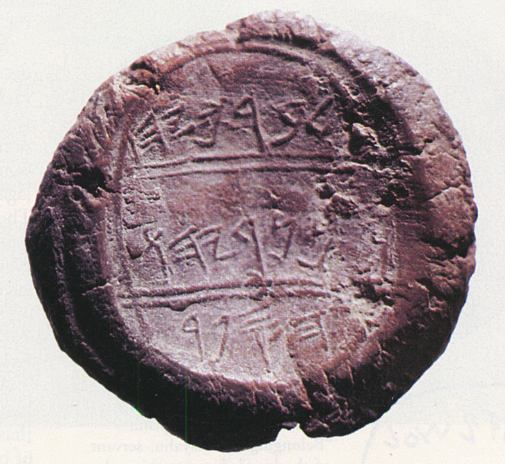
\includegraphics[scale=0.3]{Baruch_Siegel}
    \caption{Tonsiegel}
    \label{fig:Siegel}
\end{wrapfigure}

Richard Elliot Friedmann stellt die gewagte These auf, dass der Autor des Buches Jeremia dieser Autor sei. Dafür kommen laut ihn Jeremia selbst und sein Gefährte Baruch infrage. Er begründet dies textanalytisch mit einen Vergleich der Stile und Aussagen in der Deuteronomischen Historie und dem Buch Jeremia. Da Jeremia auch ein levitischer Priester in Anatoth war, dessen Vater der Finder der Buch der Thora sein könnte, nahm Friedmann dies als Grund dieser Annahme. Es ist bekannt, dass sie sehr viele seiner Lehren und Botschaften schriftlich niedergeschrieben haben. Auch wurde um 1980 von Nachman Avigad einen Siegelabdruck mit Ton gefunden, welche die Inschrift ``\textit{Eigentum von Baruch, dem Schreiber}'' trug (siehe Abb.\ \ref{fig:Siegel}). Da Jeremia und Baruch eine (vielleicht auch nur geschäftliche) Beziehung über eine längere Zeitspanne pflegten, mussten sie sich in ihren Interessen und vor allen in ihren religiösen Überzeugungen ähneln, da es sonst langfristig zu Konflikten geführt hätte, welche sich in den Schriften in Form eines stilistischen Bruchs widergespiegelt hätte. Da dieser Bruch nicht vorhanden ist, ist anzunehmen, dass zwischen Jeremia und Baruch im Inhalt ein gemeinsamer Konsens besteht. Man kann also beide als eine Einheit beurteilen. Ob Jeremia nun der ``wirkliche''  Autor ist oder nicht, spielt keine primäre Rolle.

\section{Chronistisches Geschichtswerk}
Ähnlich wie bei der Deuteronomischen Historie nimmt man an, dass die 1./2. Chronik sowie Esra und Nehemia von einen Autor geschrieben wurden und ursprünglich eine Einheit bildeten. Diese These war weitestgehend akzeptiert, wird jedoch immer mehr hinterfragt. Die Frage nach dem Verfasser ist also immer noch offen.
\\~\\
Auch wenn die Schriften textanalytisch sowie theologisch Gemeinsamkeiten aufweisen, gibt es in manchen Stellen Spuren von einer nachträglichen Bearbeitung. Eine Theorie ist, dass es einen Urautor 400 v. Chr.\ gab, der den Urtext schrieb und einen jüngeren Chronisten um 300 v. Chr., der den Urtext erweiterte, ähnlich wie Jeremia im Deuteronomischen Geschichtswerk. Diese These wird von Exegeten eher gemieden, jedoch könnte sie sowohl die Gemeinsamkeiten als auch die Unterschiede erklären.
\\
Die Frage nach dem Autor ist nicht geklärt. Jedoch kommt die aaronitische Priesterschaft infrage, da diese so schlussendlich sich ihre alleinige Macht nach dem Exil sicherte. Es ist zwar keine offizielle These und hat keinerlei Gefolgschaft, jedoch könnte Esra, gestützt auf der Annahme, dass er das Pentateuch zusammengefügt hat, das chronistische Geschichtswerk geschrieben haben. Er war ein Schriftgelehrter und genoss die Zuneigung der babylonischen Monarchie. Er besaß die Mittel und Fähigkeiten, diese Schriften abzufassen und (in einen gewissen Rahmen) um seine Interessen zu erweitern. Er könnte der Autor des Urtextes sein. Ein aaronitischer Priester könnte dann später die Schrift modifiziert haben, um Zweifel auszuräumen und/oder die Macht der Priester zu sichern oder auszubauen.
\\~\\
Zugegeben, das sind sehr, sehr weit her gegriffene Spekulationen, doch sie sind plausibel und würden sich in das bisherige Bild einfügen. Jedoch könnte es auch eine jede andere beliebige Person geschrieben haben, die literarische Fähigkeiten besaß und sich mit der damaligen Situation abfand. Wie fast im ganzen Alten Testament ist die Verfasserfrage auch hier umstritten und ein Konsens ist nicht abzusehen.

\section{Ketubim/Die Schriften}
Zu den Ketubim zählen das Buch Hiob, die Psalmen, die Sprüche, die Prediger und Hoheslied. Laut Verfassertradition wurden einige der Bücher von König Salomo geschrieben, jedoch wird heutzutage anderes angenommen. Die Verfasserfrage ist hier so schwammig, dass nur gesagt werden kann, dass die Autoren selbstständig waren. Sicherlich war der eine oder andere bereits bekannte Autor beteiligt oder die eine oder andere historische Person, jedoch kann die Verfasserfrage keineswegs geklärt werden. Man könnte dies beklagen oder die Schriften als schlichte Poesie sehen. Dies bleibt jeden selbst überlassen.

\section{Die großen Propheten}
\subsection*{Jesaja}
Die Verfasserfrage ist umstritten. Die klassische Darstellung unterteilt die Schrift in einen Protojesaja (Kapitel 1--39), einen Deuterojesaja  (Kapitel 40--55) und einen Tritojesaja (Kapitel 56--66) und ordnet allen drei Teilen einen eigenen Verfasser zu. Dies fußt auf der rationalen Annahme, dass keine Prophetie über die Lebenszeit hinweg möglich sei und dass es anscheinend schwerwiegende textanalytische Unterschiede gäbe. Jedoch ist zu kritisieren, dass für eine Schrift mit irrationale Gegebenheiten wie z.B. die Prophetie rationale Maßstäbe angewandt werden. Aus Standpunkt eines Glaubenden können Prophetien sehr wohl möglich sein und die Theologie ist eine Wissenschaft, die nicht komplett vom Glauben getrennt werden kann.
\\~\\
Die andere Theorie verfechtet diese Aufteilung und sieht die Schrift als eine Einheit an. Prophetie sei möglich und schon öfters im Alten Testament eingetreten. Auch reden Zeitzeugen und andere Schriften wie z.B. die Septuaginta immer von einen einheitlichen Jesaja. Die stilistische Unterschiede müssen auch nicht gegen eine einzigen Verfasser sprechen. Es gibt genug gemeinsame stilistische Merkmale und die stilistischen Unterschiede schließen einen einheitlichen Jesaja nicht aus. Goethes Faust I und II weisen auch stilistische Unterschiede auf und haben trotzdem zweifellos denselben Verfasser. Das gleiche kann auch auf Jesaja übertragen werden. Jesaja selber ist also der Verfasser des gleichnamigen Buches. Jesaja stammte aus einer vornehmen, judäischen Familie, wurde ca. 765--760 v. Chr.\ geboren und pflegte Kontakte zum König Usija und zu einen Priester. Er wurde von Gott berufen und ist somit göttlich inspiriert.

\subsection*{Jeremia}
Das Buch des Jeremia wurde 605/604 v. Chr.\ von den Propheten Jeremia selbst geschrieben. Jedoch diktierte er es seinen Schreiber Baruch, der es verschriftlichte. Die Übersetzungen der Septuaginta sind um ein Achtel kürzer und unterscheidet sich in der Anordnung der Kapitel als die originale hebräische Fassung, da die Übersetzer offenbar Wiederholungen raus kürzen und die Geschichten in eine chronologische Reihenfolge ordnen wollten. Die göttliche Inspiration Jeremias steht außer Frage, da Jeremia Priester war und von Gott persönlich berufen und geleitet wurde.

\subsection*{Klagelieder}
Die Klagelieder sind anonym geschrieben. Aufgrund eines ähnlichen Stils und des passenden historischen Hintergrundes ist man lange zeit davon ausgegangen, dass Jeremia der Verfasser sei. Dies ist heutzutage jedoch umstritten. Jeremia kann der Autor sein, muss es aber nicht. Die Argumente dafür und dagegen halten sich in der Waage. Da dies ein poetisches Buch ist, spielt die offene Verfasserfrage kein gravierende Rolle.

\subsection*{Ezechiel/Hesekiel}
Ezechiel war ein Priester und Prophet zur Zeit der babylonischen Verbannung. Das Buch wurde zweifelsfrei von ihm selber geschrieben. Er nennt sich selber als Autor und die Schrift hat einen durchgängig einheitlichen Stil, die einen Priester wie Ezechiel zugeordnet werden kann. Das Buch wurde 592--570 v. Chr.\ in Babylonien geschrieben. Wie Jeremia ist Ezechiel aufgrund seines Priesteramtes und seiner göttlichen Berufung göttlich inspiriert.

\subsection*{Daniel}
Bei Daniel teilen sich die Ansichten wie bei Jesaja in zwei Lager auf. Ähnlich wie bei Jesaja ist ein Grund dafür, dass Prophetie über die Lebenszeit hinaus nicht möglich sei. Mit der bereits getroffenen Annahme, dass Prophetie möglich ist, ist anzunehmen, dass der Verfasser auch wirklich der Prophet Daniel ist.Außerdem ist Daniel ein perfektes Beispiel für die Prophetie über die Lebenszeit hinweg, da Daniel bis zu der Zeit Jesus prophetiert bzw.\ einen Traum gedeutet hat. Da aber der alttestamentliche Kanon mit der Septuaginta bereits vor Jesus vollendet war, kann diese Prophetie nicht nachträglich eingefügt worden sein. Die Schriftrollen von Qumran kennen auch nur einen einheitlichen Daniel.  Es gibt Verbindungen von damaligen babylonischen Machthabern zu Daniel, deren Existenz nachgewiesen ist. Diese werden im Buch Daniel  genannt und lassen somit eine Datierung zur Zeit des Babylonischen Exils deuten. Das Buch wurde somit vermutlich um 535 v. Chr.\ in Babylonien verfasst. Daniel wurde nicht im klassischen Sinne berufen, erhielt jedoch die Gabe der Traumdeutung und war ein ergebener Diener Gottes. Man kann daher davon ausgehen, dass Daniel göttlich inspiriert war.

\section{Dodekapropheton/Kleine Propheten}
\subsection*{Hosea}
Das Buch Hosea ist eines der am schlechtesten erhaltenen Bücher. Über Hosea selber ist wenig bekannt. Die einzige Quelle über seine Person ist seine eigene Schrift. Dies lässt Zweifel zu, dass Hosea selber das Buch als eine Einheit geschrieben hat. Die Entstehung dieser Schrift ist heutzutage sehr umstritten. Es kann jedoch davon ausgegangen werden, dass weder die These, das Buch sei von Hosea selber geschrieben worden noch die These, das Buch sei eine Komposition vieler jüdischer Schriften nicht gehalten werden können. Als minimaler Grundkonsens lässt sich festhalten, dass das Buch in seiner überlieferten Gestalt eine in mehreren Phasen gewachsene planvolle Komposition darstellt. Dabei  ist es auch wahrscheinlich, dass einige Passagen auf die Reden des Hosea zurückgehen. Es ist anzunehmen, dass das Buch seine Endgestalt in Juda erhalten hat. Aufgrund der schwammigen Verfasserfrage lassen sich nur wage Rückschlüsse auf die göttliche Inspiration treffen. Es ist jedoch anzunehmen, dass Hosea und die späteren Redaktoren nach der Wahrheit Gottes gesucht hatten, d ihre Klageschriften nach Gott suchen. Es ist also möglich, dass sowohl die Autoren als auch die Redaktoren göttlich inspiriert waren.

\subsection*{Joel}
Das Buch Joel ist zweifelsfrei auf Joel selber zurückzuführen, da Petrus ihn in der Apostelgeschichte zitiert. Strittig ist die Einheit des Buches. Während die einen die Einheit befürworten, teilen die andern das Buch in zwei Teile auf, nämlich Kapitel 1 und 2 und Kapitel 3 und 4. Dies spielt jedoch eine untergeordnete Rolle, das beide Bücher zweifelsfrei auf Joel zurückzuführen sind. Auch die Datierung ist sehr umstritten und spaltet sich von der frühe vorexilischen Zeit um 800 v. Chr.\ bis zur spät-nachexilischen Zeit um 200 v. Chr.\ auf. Da es keinen König gab, bei dem der Zentralkult verehrt wurde und der Autor für die Zeit typische, aramäische Begriffe benutze ist es anzunehmen, dass Joel 400--300 v. Chr.\ geschrieben wurde. Über den Verfassungsort lässt sich keine Aussage treffen. Seine Ausdrucksweise  deutet daraufhin, dass er für sein Volk betete und laut der Überlieferung war er von Gott berufen. Folglich war Joel göttlich inspiriert, auch wenn wir wenig über seine Person wissen.

\subsection*{Amos}
Heutzutage ist die Entstehungsgeschichte zu Amos umstritten. Es wird angenommen, dass die Schrift mindestens einer Redaktion durchlaufen ist, seine Endfassung das Produkt einer nachexilischen Ära sei und drei verschiedene Profile aufweist (Am 1--2, Am 3--6, Am 7--9). Die Überlieferungen werden auf Amos zurückgeführt, jedoch sind Kapitel 1,9, Kapitel 1,11f.; Kapitel 2,4f.; Kapitel 3,7;  und Kapitel 9,8--15 nicht Amos zuzuschreiben. Umstritten ist, ob Kapitel 5,6, Kapitel 5,14f, Kapitel 8,4--7 und Kapitel 8, 11--14 auf Amos zurückzuführen sind. Die möglichen Verfasser der genannten Stellen könnten jedoch mit hoher Wahrscheinlichkeit Schüler oder Nachfolger Amos sein, die sein Werk erweitern oder neu interpretierten. Folglich wären sie genauso wie er gläubig und es ist wahrscheinlich, dass Gott sie genauso geleitet hat wie Amos selber, um eine Schrift nach seinen Vorstellungen zu gewährleisten. Die Stellen, die auf Amos zurückzuführen sind, sind aufgrund seiner Berufung göttlich Inspiriert. Bei den anderen Stellen kann keine eindeutige Aussage getroffen werden, jedoch ist eine Tendenz hin zur göttlichen Inspiration möglich. Zum Glück stammen nur wenige Verse von ihnen, sodass es nicht schwer ins Gewicht fällt.

\subsection*{Obadja}
Die Entstehung wird verschieden konstruiert. In der Regel geht man davon aus, dass Obadja in einen mehrstufigen Prozess geschrieben wurde. Dabei geht Zenger von einer dreistufigen Entstehungsprozess aus, der in der ersten Hälfte des 6. Jh v. Chr.\ anfing und am 3./4. Jh v. Chr.\ beendet wurde.	Wöhrle dagegen proklamiert bist au 17a auf einen einheitlichen Text, der in der frühhellenistischen Zeit (3. Jh v. Chr.) geschrieben wurde. Ersteres ist plausibler. Demnach wäre die erste Stufe auf Obadja zurückzuführen. Über Obadja weiß man sehr wenig. Genauso wenig weiß man, wer die anderen zwei Stufen geschrieben hat. Man kann die Autoren auf Israel eingrenzen, da Edom in dieser Schrift negativ dargestellt wird und sich ein israelitischer Autor aufgrund des Völkerkonfliktes zwischen Edom und Israel perfekt in das Bild einfügen würde. Da über die Autoren wenig bekannt ist, lassen sich keine eindeutige Aussagen über ihre göttliche Inspiration treffen. Man könnte darauf spekulieren, dass sie Juden, aufgrund ihrer schreiberischen Fähigkeiten höher gebildet und/oder deswegen Schriftgelehrte oder Priester waren, jedoch gibt es dafür keinerlei Beweise.

\subsection*{Jona}
Jona selber bezeichnet sich selbst nie als Prophet noch versteht sich die Schrift als Prophetenschrift. Die Schrift ist daher eine Prophetenerzählung in Prosaform. Eine textanalytische Analyse ergibt, dass die Schrift in der nachexilistischen Zeit anzusetzen ist. Spezifischer wird die Datierung zwischen der Perserzeit im 5. Jahrhundert v.Chr.\ bis in die hellenistische Zeit im 3. Jahrhundert v.Chr.\ angesetzt. Da aber in Jesus Sirach, eine Schrift in den Apokryphen, der Dodekapropheton erwähnt wird, in dem Jona mitvertreten ist, kann eine Datierung früher als 200 v.Chr.\ nicht möglich sein. Aufgrund der im Verschlingungsepisode und im Ninivebild aufgenommenen außerbiblischen Traditionen ist eine Datierung in die hellenistische Zeit wahrscheinlicher. Bei beiden Datierungen steht jedoch Jona als Verfasser selbst außer Frage. Längere Zeit zweifelte man die Einheitlichkeit der Schrift an, jedoch wird heutzutage die Einheit der Schrift -bis auf den eingeschobenen Psalm- nicht mehr angezweifelt.
\\~\\
Die teils sehr phantastischen Erzählungen beweisen, dass die Schrift nicht als historische Schilderung verstanden werden will. Daher stellt sich nur die Frage, ob die Botschaft selber göttlich inspiriert sei. Hier lassen sich nur wage Aussagen treffen. Da das Buch sehr wahrscheinlich zur Belehrung dient, ist es durchaus möglich, dass ein Schriftgelehrter oder ein Priester diese Schrift geschrieben hat, da diese das Wissen, die Fertigkeiten und die Autorität dazu besaßen. Da diese eine außerordentliche Verbindung zu Gott besaßen und nach seinen Willen agieren wollten, ist eine göttliche Inspiration möglich. Jedoch wissen wir anhand der Evangelien und den Geschichten rund um Jesus, dass diese -freiwillig oder unfreiwillig- auch mal entgegen Gottes Vorstellungen agierten. Die Botschaft der universalen Gnade Gottes, die auch von Jesus gelehrt wurde, beseitigt in diesen Fall die Zweifel.

\subsection*{Micha}
Das Buch Micha unterlief einen teils komplexen Entstehungsprozess, der wahrscheinlich 500 Jahre gedauert hat. Das Buch unterlief vermutlich einen fünfstufigen Entstehungsprozess, in dem die Worte des Propheten Micha aktuell blieben und lediglich neu verstanden bzw.\ neu interpretiert wurden. Der Entstehungsprozess begann im 8. Jahrhundert v.Chr.\ mit den Feldzug Sargons II.\@ gegen Philistäa und endete vermutlich in der ptolemäische Zeit im 3. Jahrhundert v.Chr.
\\~\\
Der älteste Teil des Michabuchs findet sich in Mi 1--3, wobei nach der neuesten Forschung davon auszugehen ist, dass selbst hier keine bloße Zusammenstellung von authentischen Michaworten vorliegt, sondern die Anliegen des historischen Micha durch einen Schüler- oder Sympathisantenkreis literarisch verarbeitet wurden. Diese so genannte ``Micha-Denkschrift'' aus dem 7. Jahrhundert v.Chr.\ wurde nach der Katastrophe von 586 v.Chr.\ durch 4,8--5,3 ergänzt und frühnachexilisch zu der Komposition Mi 1--5 erweitert. Mitte des 5. Jahrhundert v.Chr.\ kam die Komposition 6,1--7,7 hinzu. Im Rahmen der Endredaktion am Ende der persischen Zeit bzw.\ zu Beginn des hellenistischen Zeitalters (4./3. Jahrhundert v.Chr.) wird der Schluss des Michabuchs Mi 7,8--20 erstellt. Entsprechend der Abfolge ``Unheil-Heil'' zeigt sich für beide Teile (1, 2--5, 14 und 6, 1--7, 20), dass die Heilsperspektive jeweils eine Aktualisierung der älteren Unheilsperspektive darstellt.
\\~\\
Da der Grundbestand der Schrift auf Micha selber, einen Propheten zurückzuführen sind und die Redakteure das Ziel hatten, Gottes Worte, die durch Micha kundgetan wurden, für ihre Zeit zu deuten und zu interpretieren, ist anzunehmen, dass sowohl der Grundtext nach Micha als auch die späteren Ergänzungen göttlich inspiriert sind bzw.\ sich vom heiligen Geist haben leiten lassen.

\subsection*{Nahum}
Das Buch Nahum weist einen mehrstufigen Entstehungsprozess auf. Die Entstehung begann zw. 664--612 v.Chr.\ und endete im 4. Jahrhundert v.Chr.. Der erste Teil der Schrift wurde zur Zeit des Untergangs Thebens bis zum Untergang Ninives geschrieben. Wann die weiteren Fortschreibungen Nahums historisch zu verorten sind, ist schwer zu bestimmen. Vereinfacht lässt sich sagen, dass Nahum in zwei Blöcken geschrieben wurde. In einen richtet es sich an Ninive und dessen Zerstörung, also an den zuvor datierten Block, und im anderen an Juda selber. Letzterer Block kam zu der Zeit des Babylonischen Exils hinzu.\ in der nachexilischen Zeit wurden diese Blöcke redaktionell verwoben und um den Psalm erweitert.
\\
Da wenig über den Entstehungsprozess bekannt ist, lässt sich nur die Aussage treffen, dass die Worte, die direkt auf Nahum zurückzuführen sind, göttlich inspiriert sind, da er von Gott berufen wurde und er seine Worte verkündete. Da aber die Redaktion vermutlich nur zwei Quellen verwoben hat, ist anzunehmen, dass es sich bei den zwei Quellen um zwei verschieden Überlieferung (-sgeschichten) handelt, die beide Nahum als sprachliche Quelle als Ursprung haben und sich über verschiedene Wege verschriftlichten, bis sie zu einer Einheit zusammengefügt wurden. Daher wird die ganze Schrift göttlich inspiriert sein, da beide Blöcke auf Nahum zurückzuführen sind.

\subsection*{Habakuk}
Die Entstehung wird zwischen 625 v.Chr.\ und 605 v.Chr.\ datiert. Er hat sein Buch vermutlich in Juda verfasst, da Habakuk nicht unter der Zerstörung des Nordreiches litt. Nach dem Fund eines Kommentars zu den Buch habakuk in den Qumranhölen zweifelte man die Einheit des Buches an, da in diesen Kommentar nicht Zefanja 3 erwähnt wurde. Jedoch sind diese Vorwürfe abzuschmettern, da sich in Zefanja 1--3 textanalytisch grammatikalische, sprachliche und thematische Zusammenhänge festgestellt werden konnten. Jedoch unterlief die Schrift mehrerer Redaktionen, in denen auch geringfügige Ergänzungen gemacht wurden. So wurde einzelne Ergänzungen gemacht, um das Buch in das Dodekapropheton einzufügen und um ein ganzes Anti-Babylonisches Werk zu kreieren. Eine solche Ergänzung wären z.B. die Weherufe und Klagen. Auch wurden einzelne stilistische Eingriffe unternommen, um so die Schrift in einen Gottesdienst gebrauchen zu können. Letztendlich ist der Grundbestandteil aber auf Habakuk selbst zurückzuführen und wurde nur um liturgische und kleinere thematischen Aspekte erweitert oder neu interpretiert. Daher ist auch hier davon auszugehen, dass ähnlich wie bei Micha Habakuk selbst als Prophet als auch die Redaktoren göttlich inspiriert waren.

\subsection*{Zefanja}
In der neueren Forschung ist die Annahme weithin akzeptiert, dass das Zefanjabuch aus einer Reihe literarischer Einheiten zusammengesetzt ist und einen mehrschichtigen Redaktionsprozess verrät.Die ältesten Teile des Buches werden in die Zeit des Reformerkönigs Joschija von Juda in der zweiten Hälfte des 7. Jahrhunderts v.Chr.\ datiert. Seine jüngste Teile stammen aus dem 4./3. Jahrhundert v.Chr. Es ist anzunehmen, dass einige der früheren Textpassagen auf Zefanja selbst zurückgehen. Spätere Ergänzungen sind einerseits auch auf Zefanjas Worte zurückzuführen und andererseits redaktionellen Erweiterungen im babylonischen Exil, um das eingetretenen Gottesgericht über Juda zu dokumentieren und zu begründen. In der nachexilistischen Zeit wurden Heilsversprechungen eingefügt und das Gottesgericht universalisiert.
\\
Da durch die späteren Redaktionen das ursprüngliche Wort Zefanjas unberührt blieb und nur um weitere Aspekte erweitert wurde, ist anzunehmen, dass die Schrift göttlich inspiriert ist. Ähnlich wie bei dem Buch Micha ist anzunehmen, dass die Redaktoren göttlich inspiriert sind, weil sie bei den offenen Fragen sich von Gott haben leiten lassen.

\subsection*{Haggai}
Viele Forscher nehmen an, dass Haggai kurz nach seinen Auftreten entstanden ist. Es ist jedoch anzunehmen, das literarisch ein paar wenige Eingriffe eines Redakteurs unternommen wurden. Der Inhalt an von sich ist aber auf Haggai bzw.\ seine Reden selbst zurückzuführen. Daher ist die Datierung um um 620 v.Chr.\ anzusiedeln, da dort die Reden Haggauis präzise in der Schrift selber datiert wurden. Da Haggai ein Prophet war und somit von Gott berufen und eingesetzt, ist das Buch göttlich inspiriert, da die eingriffe rein stilistischer Natur sind.

\subsection*{Sacharja}
Das Buch Sacharja wird in in eine Proto- und Deuterojesaja eingeteilt. Ersteres umfasst Sacharja 1--9 und ist zweifelsfrei auf ihn selbst zurückzuführen. Letzteres war wahrscheinlich eine Ergänzung eines späteren Propheten, dessen Wirken zusammen mit Sacharjas zu einer Sinneseinheit zusammengefügt wurden. Der Protosacharja ist 520--518 v.Chr.\ zu datieren und der Deuterosacharja wird in die hellenistische Zeit im 3./2. Jahrhundert v.Chr.\ datiert. Da beide Schichten thematische Gemeinsamkeiten aufweisen, ist anzunehmen, dass der Verfasser des Deuterosacharja die Aussagen des Sachaarja erweiter bzw.\ vollendet hat. Daher ist anzunehmen, dass beide als Propheten oder als Prophet und als Verfasser, dessen Aussagen die eines Propheten entsprechen göttlich inspiriert sind.

\subsection*{Maleachi}
Zunächst nahm man an, dass Maleachi nicht als Name, sondern als ein Buchtitel verstanden werden muss und eine Gruppe diese Schrift verfasst habe. Heutzutage zieht man jedoch Maleachi als ein Prophet in Betracht, belegt wurde diese These jedoch nicht und wird aufgrund fehlender Belege nie belegt werden können. Die Entstehung ist eine offene und schwierige Frage. Es gibt jedoch eine Grundschicht, die auf Maleachi selbst zurückgeführt werden kann. Diese wurde dann unsystematisch um einzelne Worte ergänzt. Dadurch lassen sich spätere Redaktoren praktisch nicht ermitteln. Die Frage nach der göttlichen Inspiration ist also schwammig beantwortbar. Die Grundschicht wird aufgrund dessen, dass Maleachi als Prophet berufen war, göttlich inspiriert sein, jedoch lässt sich keine Aussage über die Redaktoren treffen. Diese scheinen aber die Schrift um nur einige Gesichtspunkte erweitert zu haben, jedoch in keiner Weise, dass ganze neue Aspekte geschaffen wurden.


\section{Schlussbetrachtung}
Die Entstehungsprozesse der einzelnen Schriften sind teilweise sehr Komplex und weisen gerade im Dodekapropheton einen vielschichtigen und komplexen Entstehungsprozess auf, der hier nur auf das simpelste runter gebrochen wurde. Einige Schriften wie z.B. das Pentateuch, aber auch des Deuteronomischen Geschichtswerkes sind extrem Kontrovers und die eine Wahrheit gibt es bei dieser Thematik nicht. Glücklicherweise konnten meistens die Grundbestandteile der Schriften auf Propheten oder andere von Gott berufene Persönlichkeiten zurückgeführt werden, sodass der Kern göttlich inspiriert ist. Die Grundtheologien der einzelnen Schriften blieben unverändert.
\\~\\
Doch in den meisten Fällen steckt noch eine langwierige Redaktionsgeschichte dahinter, die von den aktuellen historischen Ereignissen geprägt wurden. Gerade wenn es um Ergänzungen von Schriftgelehrten oder Priestern geht, die v.a. Gesetze, Bräuche oder Machtverhältnisse beinhalten, muss die Schrift kritisch betrachtet werden. Nicht selten versuchten Eliten, durch gezielte Geschichtsschreibung die Missstände zu verdecken, auch wenn größere Lügen hier nicht entdeckt wurden oder an anderen Stellen der Bibel richtig gestellt werden.
Ein großer Knackpunkt vor allen bei den großen Propheten sind die Einheit einzelner Bücher. An Stellen wie z.B. dem Pentateuch ist es angebracht, jedoch werden durch fragwürdige Annahmen z.B. Bücher wie Jesaja aufgeteilt. Schlussendlich muss sich aber jeder selber entscheiden, ob er an einer Einheit oder einer Aufteilung der Schriften festhält.
\\~\\
Erstaunlich ist, wie bei Entstehungsgeschichten, die sich teilweise über ein halbes Jahrtausend erstreckten, der Kernbestand unverändert blieb und immer auf eine von Gott eingesetzte, berufene oder geleitete Person zurückführen lässt. Die Ergebnisse stellen auf den ersten Blick die Glaubwürdigkeit des Alten Testaments in Frage, jedoch gibt es im Vergleich zu anderen Werken kein vergleichbares Werk von Geschichtsschreibung. Das Alte Testament ist für die damaligen Verhältnisse als Geschichtsschreibung präzise und einzigartig! Natürlich Bedarf es bei der Exegese eine grundkritische Einstellungen, um Fehler durch Menschenhand ausfindig zu machen. Letztendlich bleibt die Bibel Gotteswort in Menschenwort und Menschenwort ist fehlbar.
\chapter{Das Neue Testament}
Ein römischer Kleriker behauptete, dass die Existenz Jesu historisch bewiesen sei. Darauf folgte Kritik und sogar eine Anzeige, welche sich jedoch verlaufen hat. Auch wenn die katholische Hierarchie fragwürdig ist, ist diese  Aussage jenes Glaubensbruders sehr zutreffend. Die Existenz Jesu ist mehrfach überliefert und bewiesen, auch von dritten, unabhängigen Quellen. Es folgen ein paar Exzerpte:
\medskip
\begin{center}
    \begin{minipage}{0.9\linewidth}
        \small
        ``Christus war unter des Tiberius Führung vom Procurator Pontius Pilatus hingerichtet worden''
        \\ \footnotesize{\textit{(Cornelius Tacitus, Annalen, Phaidon Verlag, Wien 1935, S 740; XV.\@ 44)}}\small
        \\~\\
        „Um diese Zeit lebte Jesus, ein weiser Mann, wenn man ihn überhaupt einen Menschen nennen darf. Er vollbrachte nämlich ganz unglaubliche Taten und war der Lehrer aller Menschen, die mit Lust seltsame Dinge aufnahmen. So zog er viele Juden und auch viele Heiden an sich. Dieser war der sogenannte Christus. Und obgleich ihn Pilatus auf Betreiben der Vornehmsten unseres Volkes zum Kreuzestod verurteilte, wurden doch seine früheren Anhänger ihm nicht untreu. Denn er erschien ihnen, wie sie behaupteten, am dritten Tage wieder lebend, wie gottgesandte Propheten dies und tausend andere wunderbare Dinge von ihm vorhergesagt hatten. Und bis auf den heutigen Tag besteht das Volk der Christen, die sich nach ihm nennen, fort.“
        \\ \footnotesize \textit{(Flavius Josephus, Antiquitates Judaicae, Verse 63–64)} \small
        \\~\\
        Im Britischen Museum befindet sich das Manuskript eines Briefes, der etwa 73 n. Chr.\ von einem Syrer namens Mara Bar-Serapion verfasst worden ist. Er erwähnt die Hinrichtung von Sokrates, Pythagoras und Christus und zeigt, dass die Verfolgung von weisen Männern nur Unglück bringt.
        \\ \footnotesize \textit{(F. F. Bruce, Die Glaubwürdigkeit der Schriften des Neuen Testaments, Verlag der Liebenzeller Mission, 1976, S. 122)} \small
        \\~\\
        Lucian, ein Satiriker des 2. Jh.\ n. Chr.\ bezeichnete Jesus als ``den in Palästina gekreuzigten Menschen''
        \\ \footnotesize \textit{(Lucian, Über das Lebensende des Peregrinus, in Lucian Bd. 2, S. 9, Griechische und römische Klassiker, Langenscheidt Verlag, Berlin 1855--1920, Bd. 36)} \small
        \\~\\
        ``Da die Juden unter ihrem Anführer Chrestos (d.h. Christus) beständig Unruhe anstifteten, vertrieb er (d.h. Claudius) sie aus Rom''
        \\ \footnotesize \textit{(Gaius Suetonius Tranquillus, Leben der Caesaren, Claudius, Artemis-Verlag, Zürich 1955, S. 296; § 25)} \small
    \end{minipage}
\end{center}

\begin{center}
    \begin{minipage}{0.9\linewidth}
        \small
        Um 150 n. Chr.\ schickte Justin der Märtyrer eine Verteidigungsschrift des Christentums an Kaiser Antonius Pius und verwies ihn an den Bericht des Pilatus, der in den kaiserlichen  Archiven aufbewahrt wurde: ``Dass dies so geschehen ist, könnt ihr aus den unter Pontius Pilatus angefertigten Akten ersehen''
        \\ \footnotesize \textit{(Justin der Märtyrer, Apologien, Kösel Verlag, München 1913, S 48 f.u. 61; I.35)} \normalsize
    \end{minipage}
\end{center}
\medskip
Egal, ob diese Überlieferungen zweifelsfrei sind oder nicht, allein der Fakt, dass so viele Quellen -viele davon aus dritter Hand- von Jesus berichten, bestätigen dessen Existenz. Manche gehen soweit, dass sie sagen, dass man die Evangelien aus dritten Quellen fast komplett rekonstruieren könne. Die Gefolgschaft Jesu war zahlenmäßig groß und so auch die Überlieferungen. Schlussendlich gibt es mehr Quellen, die Jesus Existenz und somit sein wirken bestätigen als bei Gaius Julius Cäsar, dessen Existenz und Geschichten nicht angezweifelt werden. Heutzutage \emph{weiß} man, dass Jesus existiert hat.


\section{Die synoptischen Evangelien}
\begin{figure}[h]
    \begin{center}
        
\includegraphics[width=\linewidth]{Zwei-Quellen-Theorie}\label{Quellentheorie}
        \caption{Schematisches Schaubild der Zwei-Quellen-Theorie}
    \end{center}
\end{figure}
Die am meisten anerkannte und plausibelste Theorie für die Überlieferung der synoptischen Evangelien ist die sogenannte Zwei-Quellen-Theorie. In dieser wird angenommen, dass eine frühere Fassung des Markus-Evangeliums (Urmarkus) die älteste Überlieferung darstellt und sowohl Lukas als auch Matthäus als Basis gedient haben. Dies erklärt auch die meisten Übereinstimmungen zwischen Markus, Lukas und Matthäus.\\

Jedoch gibt es auch (teilweise wortwörtliche) Übereinstimmungen  zwischen Lukas und Matthäus, welche jedoch nicht im Markus-Evangelium vorkommen. Dies wird durch die hypothetische Größe der Logienquelle erklärt. Diese vermutlich schriftliche Quelle soll den beiden Evangelisten als zweite Quelle gedient haben, welche Markus nicht zugänglich war und beschränkt sich größtenteils auf die Sprüche bzw. Reden Jesu. Jedoch wurde bis heute diese Quelle nicht gefunden und muss über die Zeit durch Verwitterung, Verfall und mutwillige Zerstörung durch z.B. Krieg vernichtet worden sein. Solange diese Quelle nicht geborgen wird, wird diese Theorie ein Erklärungsversuch ohne Beweis bleiben.\\

Zuletzt besitzen sowohl das Lukas- als auch das Matthäusevangelium beide Passagen, die in den anderen Evangelien nicht vorkommen. Dies wird mit weiteren Quellen, dem Sondergut erklärt. Dies sind mündliche oder schriftliche Quellen, auf die nur die jeweiligen Verfasser Zugriff hatten. Auch diese wurden noch nicht gefunden und sind hypothetische Größen.
\\~\\
Die wohl größte Schwäche sind die hypothetischen Quellen, welche nicht erhalten sind. Jedoch ist die Annahme einer gemeinsamen Logienquelle und der Sondergüter plausibel, da alle Verfasser sich verschiedener Quellen bedienen mussten. Deutlich wird dies am Anfang des Lukas-Evangeliums, in dem Lukas davon berichtet, wie er die verschiedenen Quellen zusammengetragen und verschriftlicht hat. Und da damals die Anzahl der Überlieferungen limitiert waren, ist die Wahrscheinlichkeit einer gemeinsamen Logienquelle groß. Wie sich heute jeder Schüler bei einer Recherche bei einer gemeinsamen Quelle namens Wikipedia bedient und dann noch zusätzlich weiterer Quellen, so bedienten sich damals Lukas und Matthäus einer gemeinsamen Quelle X und ihrer eigenen zusätzlichen Sonderquellen.\\

Ein weiterer Kritikpunkt ist, dass im Markus-Evangelium Passagen aufzufinden sind, die von Lukas und Matthäus nicht übernommen wurden. Ein Grund kann sein, dass diese Passagen nach dem Verfassen der anderen Evangelien hinzugefügt worden sind und heutzutage eine überarbeitet Fassung (Deuteromarkus) des Urtextes (Urmarkus) vorliegt. Auch erklärbar sind diese Passagen als redaktionelle Gründe von Lukas und Matthäus, weil sie z.B. als anstößig empfunden wurden. Jedoch erklärt dies nicht alle Passagen und es ist schwierig, eine befriedigende und anerkannte Antworten für dieses Problem zu finden.\\

Der letzte nennenswerte Kritikpunkt sind die Minor agreements. Diese sind Passagen, die bei Lukas und Matthäus übereinstimmen, sich jedoch zu Markus unterscheiden. Dabei kann es sich um stilistische Änderungen oder Auslassungen handeln. Diese sind mit redaktionellen Gründen und stilistische Verbesserungen zu erklären. Ein weiterer Erklärungsversuch ist, dass  die Verfasser eine Urfassung (Urmarkus) des Markus-Evangeliums zur Verfügung hatten und die heutige Überlieferung eine überarbeitete Fassung (Deuteromarkus) der Schrift ist.\\

Auch wenn die 2-Quellen-Theorie nur ein ein Erklärungsversuch mit seinen genannten Schwachstellen ist, ist diese Theorie die plausibelste und erklärt am Besten die Überlieferung der drei synoptischen Evangelien. Zudem wurden zur damaligen Zeit Nachrichten, wie es heute in manchen ländlichen Gebieten auch noch üblich ist, per Mundpropaganda weitergegeben. Der Verdacht der Verfälschung ist sicherlich angebracht, jedoch konnten sich die Menschen damals die Worte fast wortwörtlich merken, da die traditionelle Mundpropaganda das Gedächtnis dazu trainiert bzw.\ getrimmt hatte.\\

Da das Lukasevangelium und das Matthäusevangelium auf der (vermutlichen) Logienquelle, den Sondergütern und dem Markus-Evangelium basieren und letzteres als einzige Quelle überliefert ist, ist das Markus-Evangelium am Besten für eine Untersuchung geeignet. Die Ergebnisse der Untersuchungen lassen sich größtenteils auf die anderen zwei Evangelien übertragen. Unbefriedigend ist der Sachverhalt, dass die zweite Quelle nicht für eine Untersuchung zur Verfügung steht. Deshalb wird ein zweite Untersuchung des Matthäus- und des Lukasevangeliums vonnöten sein.

\subsection*{Markus-Evangelium}
Laut alt-kirchlicher Überlieferung wurde das Markus-Evangelium von Johannes Markus geschrieben. Er soll der Dolmetscher von Petrus gewesen sein. Nach dieser Auffassung würde das Evangelium direkt nach Jesus Tod geschrieben worden sein und den direkten Überlieferung der Apostel zu Grunde liegen. Auch wenn es einfacher wäre, an diese Version zu glauben, gibt es Widersprüche, die dies widerlegen könnten.
\\~\\
Anzuzweifeln ist die direkte Verbindung zu Petrus. Wäre der Autor ein Dolmetscher von Petrus gewesen, hätte er von ihm wahrscheinlich mehr berichtet, da er mit ihm mehr im Kontakt als mit den übrigen Jüngern stand und es nahe steht, dass das meiste Material des Autors von Petrus hätte stammen müssen. Jedoch wird Petrus in Markus-Evangelium nicht hervorgehoben und seine Rolle wird traditionell dargestellt. Dies steht im Widerspruch zur direkten Verbindung zu Petrus. Es ist also anzuzweifeln, dass der Autor mit Petrus oder den Aposteln im engeren Kontakt stand. Die Identität des Autors ist unbekannt. Jedoch kann auf textanalytischer Basis Informationen über den Autor gesammelt werden, um den Kreis der möglichen Autoren einzuengen und Aussagen über den Autor treffen zu können.
\\~\\
Der Autor war mit großer Wahrscheinlichkeit ein Heidenchrist, d.h.\ er gehörte vor seiner Bekehrung zum (frühen) Christentum nicht dem Judentum an. Er glaubte demnach vor seiner Bekehrung nicht an den Gott Jahwe und auch nicht daran, dass eben dieser eine Gott einen Sohn auf die Erde geschickt hat, um sein Volk bzw.\ die Menschheit zu retten. Auch teilte er nicht die Geschichte Israels mit Gott. Für ihn musste vor der Bekehrung das Judentum suspekt gewesen sein, sodass er seine alte Religion beibehielt. Ihm war das Judentum fremd. Nachdem er von den Geschichten von Jesus Christus, den Messias, gehört hatte, hätte er seine alte Religion beibehalten und die Berichte anzweifeln können. Der Autor hatte mehr Gründe, die Berichte negativer aufzugreifen und darzustellen als die realen Ereignisse. Aber die Schilderungen haben anscheinend das Gegenteil bewirkt. Er hat sich vermutlich dadurch seiner eigenen Religion fremd gefühlt und dem Rücken gekehrt, einer Religion, an die er sein gesamtes Leben geglaubt hatte. Er konnte sich mehr mit Jesus Christus bzw.\ mit dem Christentum identifizieren. Seine Motivation für die Verschriftlichung war die Begeisterung für seinen neu gewonnen Glauben, der höchstwahrscheinlich sein Leben besser erfüllt hatte als seine alte Religion. Er vollzog einen Wandel von ein Kritiker zum Nachfolger Jesu. Von einer mutwilligen, ungerechtfertigten und unreflektierten Beschönigung der Bibel durch den Autor kann also kaum gesprochen werden.
\\~\\
Funde aus den Qumranhölen belegen, dass das Markus-Evangelium vor dem jüdischen Krieg (um 68 n. Chr.) entstanden sei. Die Verschriftlichung muss also davor stattgefunden haben. Im (fiktiven) Worst-Case-Szenario muss die Verschriftlichung mit der Annahme, dass der Arbeitsprozess ein Jahr dauert, 67 n. Chr.\ stattgefunden haben. Demnach würden seit dem Tod Jesu ca. 30 Jahre vergangen sein, also ca.\ eine Generation. In dieser Zeitspanne predigten die Apostel selber das Evangelium. Die Wahrscheinlichkeit liegt nahe, dass der Autor einer der Apostel begegnet ist oder zumindest zu seiner Zeit noch gelebt haben (Petrus starb vermutlich 64--67 n.Chr.). Es ist jedoch anzunehmen, dass das Markusevangelium davor geschrieben wurde.
\\
Es besteht also die Möglichkeit, dass der Autor das Evangelium direkt von den Apostel unverfälscht gehört und verschriftlicht hat. Angesichts der Bewegung der Urgemeinden und der Missionarsmissonen der 12 Apostel wäre dies nicht abwegig. Wäre dies trotzdem nicht der Fall, dann müssten die Berichte durch dritte mündlich überliefert worden sein. Folglich liegt der Verdacht der Verfälschung nahe. Da zu der Zeit die meiste Geschichten mündlich überliefert wurden, war das Gehirn dementsprechend geprägt und daran gewöhnt. Die Menschen konnten sich die Überlieferungen teilweise wortwörtlich merken und unverfälscht weitervermitteln, wie es heute in sehr ländlichen Gegenden der Erde teilweise immer noch üblich ist. Der einzige Grund zur Verfälschung wäre die Instrumentalisierung der Berichte. Jedoch war das frühe Christentum faktisch machtlos und wurde sogar verfolgt. In den meisten Regionen gab es andere Religionen, die dominanter waren. Dort wäre eine eigennützige Instrumentalisierung ertragreicher gewesen. Eine schwache Religion zu Instrumentalisieren ergibt wenig Sinn.

\subsection*{Matthäusevangelium}
Laut Verfassertradition wurde das Matthäusevangelium von den Jünger Matthäus verfasst. Ähnlich wie bei Markus ist diese Annahme vermutlich falsch und der Verfasser unbekannt. Der Autor war vermutlich ein christlicher Schriftgelehrter. Die Indizien dafür sind der Umgang mit den Alten Testament als auch der literarisch kunstvolle Aufbau des Evangeliums. Die Bibel wurde vermutlich in Syrien, genauer gesagt Antiochia geschrieben. Da in der Schrift die Zerstörung des Tempels und der judäische Krieg vorausgesetzt ist, wird die Verfassung auf 80--90 n.Chr.\ datiert.
\\~\\
In der Forschung ist die Frage umstritten, ob das Evangelium in einem juden- oder heidenchristlichen Milieu entstanden ist. Jedoch wurde die Schrift anscheinend für eine judenchristliche Gemeinde geschrieben. Auch er ist der Ansicht, dass das Heil für alle Völker gilt und kritisiert das damalige Judentum. Grund für die Kritik gab es genug. Er hat sich seiner alten Religion abgewandt und einer ``reformierten'' Fassung des Judentums (das spätere Christentum) zugewandt. Für ihn war die Lehren Jesu die Wahrheit und vor allen die Lehren der Pharisäer veraltet oder falsch. Ähnlich wie beim Markusevangelium ist es wahrscheinlich, dass der Verfasser einer der Apostel gehört hat und somit die Überlieferungen kaum verfälscht wurden. Nach der Zwei-Quellen-Theorie beruft sich Matthäus auf Markus und seinen Sondergut. Dass sich sein Sondergut direkt oder indirekt auf die Apostel beruft, ist wahrscheinlich, da die Apostel höchstens seit 30 Jahren tot sein konnten, was in einer althistorischen Schrift eine minimale Zeitspanne ist.  Auch ist das Christentum zu der Zeit faktisch machtlos, was das Argument der Instrumentalisierung der Religion entkräftet. Er hatte keinen Grund, die Schrift zu verfälschen. Er setzte lediglich nur andere Schwerpunkte in seinen Evangelium. Es ist anzunehmen, dass die Überlieferungen den Originalgeschichten entsprechen. Ausnahmen sind stilistische Ausarbeitungen wie die Symbolzahlen, welche eine Interpretation aber nur geringfügig beeinflussen können.

\subsection*{Lukasevangelium und Apostelgeschichte}
Laut Verfassertradition war Lukas ein Arzt und Begleiter des Paulus. Ob Lukas ein Schüler oder nur ein Begleiter Paulus war, ist umstritten. Jedoch verweigert Lukas Paulus den Titel des Apostel. Deswegen ist es wahrscheinlicher, dass Lukas ein Begleiter oder Freund des Paulus war. Es ist schwierig, ihn einer Gruppe zuzuordnen. Ein ärztliches Interesse lässt sich aus der Schrift nicht begründen, dennoch war er wahrscheinlich hoch gebildet. Er war also kein Arzt. Er war kein Judenchrist, da er keine semitischen Begriffe verwendet und durch griechische ersetzt. Wahrscheinlich war er ein ``Gottesfürchtiger'', welcher mit dem Judentum sympathisierte, aber sich nicht zu diesen bekehren lies. Aber mit großer Sicherheit war er wie Markus ein Heidenchrist. Die Verfassung ist um 70--90 n.Chr.\ zu datieren.
\\~\\
Wie bei Matthäus und Markus ist eine Instrumentalisierung aus den gleichen Gründen unwahrscheinlich. Er wurde vermutlich vor Matthäus und nach Markus geschrieben. Dass sein Sondergut sich auf die Apostel in erster oder zweiter Ebene beruft, ist wie bei Markus und Matthäus sehr wahrscheinlich. Auch er hatte keinen Grund, die Überlieferungen zu verfälschen.

\section{Johannesevangelium}
Das Johannesevangelium unterscheidet sich grundlegend von den synoptischen Evangelien und muss in seinen Entstehungsvorgang als eigenes Werk betrachtet werden. Dass Johannes ein Augenzeuge war, ist eher unwahrscheinlich. Dafür weist die Schrift zu reflektierende Merkmale auf. Dies spricht eher von einer zeitlichen Distanz seit dem Wirken Jesu. Die Schrift wurde vermutlich 90--100 n. Chr.\ in Syrien oder Ephesus verfasst. Der Autor stammt vermutlich aus einen judenchristlichen Milieu, da dreimal der Ausschluss aus der Synagogengemeinde als Folge des Bekenntnisses zu Jesus als dem Christus erwähnt wird. Textanalytisch kann man sagen.\ dass Johannes nicht von einer Person geschrieben wurde, sondern von einen Urautor, einer sogenannten ``johanneischen Schule'' (Kapitel 15, 16 und 17) und dem Herausgeber bzw.\ den Redakteur (Kapitel 21).
\\~\\
Der Urautor lässt sich schwer identifizieren. Vermutlich war er ein Judenchrist. Da er von den Ausschluss aus der Synagogengemeinde, sprich der Judengemeinde schreibt, liegt es nahe, dass er dies selbst erlebt haben könnte. Folglich stand er vor einer Wahl: Seine alte Religion, an die er sein bisheriges Leben geglaubt hatte, beibehalten oder sich dem neuen Christentum zuwenden. Er stand wie alle Judenchristen im Konflikt und wägte ab. Er wandte sich einer neuen Religion zu. Er befand diese für wahr. Folglich hatte er keinen Grund, sich seine neue Religion schönzureden oder zu verfälschen. Er hatte sich selbst entschieden. Es liegt nahe, dass seine Gedanken und Entscheidungsgründe für die Bekehrung in die Schrift mit eingeflossen ist. Dies würde auf den Schwerpunkt auf Jesus als Offenbarung erklären. Da das Evangelium die Struktur der synoptischen Evangelien besitzt, wird angenommen, dass der Autor diese kannte. Seine Schrift kann daher entweder als Kritik der alten Überlieferung zu sehen sein oder als Vertiefung. Auf jeden Fall soll seine Schrift eine Alternativversion der synoptischen Evangelien sein.
\\
Die johanneische Schule lebte in einen potentiell aggressiven Umfeld. Die Schule grenzt sich vom Judentum in seinen Bräuchen ab, leugnet dieses aber nicht komplett. Durch die spätere Abfassung ist es möglich, dass sowohl Johannes als auch seine Gemeinde eine zusätzliche Anzahl von Quellen, die in der Zeit um und nach der Verfassung der synoptischen Evangelien entstanden und/oder gefestigt hatten, zur Verfügung hatte. Eine zusätzliche hypothetische Quelle (-nsammlung) X ist also plausibel, jedoch gibt es keine überlieferten Manuskripte davon.
\\~\\
Die Frage der historischen Korrektheit und der Glaubwürdigkeit der Evangelien (inklusive der Apostelgeschichte) ist also geklärt. Anzumerken ist, dass es vollständige Manuskripte aller dieser Schriften gibt und die Zeitspanne zwischen dem Wirken Jesu und der Verschriftlichung verhältnisweise sehr klein ist. Die Evangelien und auch die Bibel wird oft zurecht als die historisch gesehen beste Geschichtsschreibung gesehen, trotz der Missstände im Mittelalter und der vielen Übersetzungen.

\section{Jesus Christus ist der Messias}
An Jesus Existenz und der Glaubwürdigkeit der Evangelien gibt es -wenn man die Quellen wie in meinen Falle als wahr bzw.\ glaubwürdig betrachtet- nichts mehr zu zweifeln. Jedoch kann man anzweifeln, dass Jesus nicht wirklich Gottes Sohn war, sondern z.B. ein kluger Hassprediger. Folglich wären die Lehren Jesus nicht die Worte Gottes, sondern die Worte eines ``Ketzers''. Diesen Zweifel gilt es zu beseitigen. Jedoch bewegen wir uns nun in einen Bereich, wo es kein richtig oder falsch gibt, oder kurz gesagt: Wir bewegen uns in einen Bereich, an dem man glaubt oder nicht glaubt. Auch aus diesen Grund werden die traditionelle Gottesbeweise ignoriert und alternative Erklärungen betrachtet.
\\~\\
Einerseits ist Jesus ein Nachkomme von König David. Der König, der von Gott auserwählt wurde, um sein Volk  zu vereinen. Gott schloss mit David den Davidischen Bund und gewährte ihm und seine Familie bedingungslos den Thron über sein Volk. Nach der Auflösung des Bundes durch den Untergang der davidischen Dynastie könnte dieser Bund auf Jesus übertragen oder erneuert worden sein. Er gehört also zumindest einer Familie an, die von Gott ``auserwählt'' wurde, um sein Volk zu leiten, politisch und religiös.
\\~\\
Ein anderer Punkt ist die Geburt Jesu oder besser gesagt die Schwangerschaft der Jungfrau Maria. Schenkt man den Überlieferungen Glauben, damals gab es ja noch keine Schwangerschaftstests, so wurde Jesus ohne leiblichen Vater geboren. Dies legt Nahe, dass der Vater  einer übernatürlichen Natur zuzuordnen ist. Jesus Vater muss also übernatürlicher Natur sein, was eine direkte Beziehung zu einer übernatürlichen Macht herstellt, also zu Gott.
\\~\\
Des weiteren ist das Wirken Jesu selbst zu betrachten. Die Taten und Lehren von Jesus prägen uns bis heute. Seine Werte und Lehren sind in den meisten, wenn nicht in allen, demokratischen Verfassungen verankert, der legitimisten Herrschaftsform. Seine Lebensweise, wie er sie verkündet und gelebt hat, hat nachweislich für tausende, wenn nicht Millionen Menschen eine positive Lebenswende dargestellt. Die Wunder, die Jesus gewirkt hat, sind einzigartig und auch umstritten. Diese Taten selber kann man für die damaligen Verhältnisse als übernatürlich zuordnen. Klar, dies könnte auch ein einzigartiger Mensch gewesen sein, aber für mich ist dieses Verhalten übernatürlich und ein Beweis dafür, dass Jesus Gottes Sohn war, ist und für immer sein wird.
\\~\\
Einzeln mögen die Gedankengänge keine große Aussagekraft haben, aber als Ganzes kann man es als eine plausible Erklärung sehen. Schlussendlich sind dies nur wage Spekulationen und jeder muss selbst entscheiden, ob Jesus Gottes Sohn bzw.\ der Messias ist. Dies macht das Glauben zum Glauben und nicht zum Wissen.
\section{Paulinischen Briefe}
Die Paulinischen Briefe wurden größtenteils von Paulus selbst verfasst. Paulus ist wie Jesus eine historische Person und bekannte sich zu seinen Schriften. Zum ersten mal im Neuen Testament lässt sich der Verfasser identifizieren und überprüfen. Er ist greifbar und nicht nur eine nebulöse, hypothetische Gruppe. Jedoch sind laut historisch-kritischer Bibelforschung nicht alle paulinischen Briefe von Paulus persönlich abgefasst worden, sondern von seiner Gefolgschaft oder Schülern. Die Briefe wurden 51--62 n.Chr.\ geschrieben.

\subsection*{Protopaulinischen Briefe}
Die protopaulinischen Briefe sind die Schriften, die laut historisch-kritische Exegese auf Paulus selbst zurückgeführt werden können. Dazu zählen der 1. Thessalonicher, 1./2. Korinther, Philemon, Philipper, Galater und Römer. Die Schriften wurden ca. 55--61 n.Chr.\ abgefasst.
\\~\\
Paulus war vor seinen Missionsreisen ein Verfolger der Christen. Er wollte nicht den christlichen Glauben verbreiten, er wollte es auslöschen. Für ihn war alles eine Lüge. Wenn man den Überlieferungen Glauben schenkt, dann begegnete Paulus Jesus. Die Folge war seine Bekehrung. Entscheidend ist, dass es ein Ereignis ihn seinen Leben gab, der ihn radikal sein Leben ändern ließ. Ein Ereignis von großen Ausmaß. Im Grunde lebte er im kompletten Gegensatz zum alten Paulus. Es gibt nicht viel, was als solch ein großes Ereignis in Frage kommt, um aus einen Feind einen Nachfolger zu machen. Möglich wäre ein überzeugender Christ, der eine (fast schon nahezu übermenschliche) theologische Kenntnisse oder Fähigkeiten besitzen muss oder eine übernatürliche Macht: Jesus Christus. Von daher ist das Erscheinen von Christus plausibel, aber dennoch Glaubenssache. Schlussendlich ist entscheidend, dass Paulus danach ein Überzeugter Anhänger wurde, sein Leben für die Mission riskierte und schlussendlich auch damit bezahlte. Solch eine Entscheidung ist schwerwiegend und will überdacht werden. Solch eine Entscheidung trifft man einzig aus Überzeugung, in seinen Falle Überzeugung an Gott in seiner Dreieinigen Form.
\\~\\
Da Jesus ihn berufen hat, steht es nahe, dass er auch von ihn geleitet wurde, auch in seinen Worten. Seine Überzeugung ist Begründung genug dafür, dass er die Lehren, die er verbreitet hat, nicht verfälscht hat und im theologischen Sinne glaubwürdig ist. Er wird zurecht als erster christlicher Theologe bezeichnet, dessen Existenz historisch überliefert ist.

\subsection*{Deuteropaulinischen und Pastoralen Briefe}
Die deuteropaulinischen Briefe sind die Schriften, die laut historisch-kritischer Exegese nicht auf Paulus selbst, aber auf seine sogenannte Schule zurückzuführen ist. Zu ihnen zählen die Kolosser, die Epheser, 2. Thessalonicher, 1./2. Thimotheus und Titus. Die Schriften wurden 70--100 n.Chr.\ geschrieben, nach dem Tod von Paulus. Da Paulus vermutlich seine Schüler gelehrt und ihnen seine Theologien vermittelt hat, werden diese Paulus und so Jesus Lehren gekannt und beherrscht haben. Es gibt also zwei Szenarien: Die paulinische Schule hat nach seiner Theologie sein Werk und seine Mission fortgesetzt oder sie haben die Briefe und somit den Glauben wissentlich instrumentalisiert. Ersteres Szenario würde die Glaubwürdigkeit (in einen begrenzten Rahmen) bestätigen und letzteres widerlegen.
\\~\\
Durch die Betrachtung der damaligen Umstände ist ersteres wahrscheinlicher. Zur damaligen Zeit befand sich das Christentum im Umbruch. Vieles wurde angezweifelt oder war strittig. Die Gründergeneration war gestorben. Unangefochten waren jedoch die ersten Führungspersönlichkeiten des christlichen Glauben, also auch Paulus. Durch das damalige Post- und Nachrichtensystem war den meisten Gemeinden der Tod von Paulus nicht bekannt. Seine Schule stand vor einer Wahl: Seinen Tod verbreiten mit dem Risiko, dass ihre Inhalte und Briefe angefochten werden könnten oder unter seinen Namen seine Theologie weiterverbreiten, welche dann unangefochten akzeptiert werden könnten. Eines war klar: Seine Arbeit musste fortgesetzt werden. Und dies war einfacher mit den sogenannten 				Pseudepigraphen, also indem sie ihre Schriften in Namen des toten Paulus verbreiteten.
\\
Zudem ehrte man damals seine Lehrer und/oder Vorbilder, indem man sein eigenes Werke, welches nach seinen Vorbild geschrieben wurde, in seinen Namen veröffentlichte. Damit zollte man ihn seinen Respekt. Sicherlich waren damals viele falsche Briefe im Namen von Paulus im Umlauf, jedoch sind diese nicht die Deuteropaulinischen- und Pastoralen Briefe.
\\~\\
Die paulinische Schule war trivial gesehen Paulus Anhänger und Nachfolger. Sie gaben ihr damaliges Leben, ihr Broterwerb und ihr soziales Umfeld auf, um sich Paulus anzuschließen. Sie begaben sich auf eine Reise der Unsicherheit, immer mit den Risiko des Todes. Sie wurden sicherlich verfolgt und bedroht. Dennoch hielten sie zu Paulus und so zu Jesus. Ihre Motivation für die Gefolgschaft war demnach Überzeugung, Begeisterung, Vertrauen oder ähnliches. Würden sie nun seinen Namen instrumentalisieren, um einen Eigennutzen daraus zu ziehen, dann wäre ihr Antrieb purer Egoismus und Machtgeilheit. Dieser Antrieb würde sich aber nicht mit ihrer Motivation für die Gefolgschaft decken. Ein machtgeiler Egoist hätte nicht sein altes Leben aufgegeben und sein Leben für eine Mission riskiert. Eine eigennützige Instrumentalisierung des Namens Paulus kann also ausgeschlossen werden.
\\~\\
Die paulinische Schule nutzte also Paulus Namen, um seine Theologie weiterzuverbreiten und so das Christentum vor Irrlehren zu schützen und ein wenig Stabilität zu geben, soviel, wie es unter den damaligen Umständen der Verfolgung und der Umbrüche möglich war. Dies war der Grund für die Pseudepigraphen. Der Unterschied zwischen den Deuteropaulinischen und Pastoralen (auch Tritopaulinischen) Briefen war, dass für die Pastoralen Briefe die Protopaulinischen Briefe bzw.\ deren Inhalt sowohl der paulinischen Schule als auch der Empfänger bekannt gewesen sein muss.

\section{Katholischen Briefe}
Die katholischen Briefe sind die Briefe, die nicht an eine spezifische Gruppe oder Gemeinde gerichtet sind. Sie sind an die Kirche allgemein gerichtet und heißen deshalb katholisch im Sinne von allumfassend oder allgemein. In den Briefen werden selten Verfasser genannt oder es sind Pseudepigraphen. Wegen den schwammigen Eingrenzung der Autoren lassen sich keine Aussagen über ihre Motivation treffen außer diese, die auch bei den zuvor genannten Verfasser getroffen wurden. Deshalb werden im Folgenden nur der Autorenkreis eingegrenzt und nicht wie üblich die Autoren überprüft, da sich die Ergebnisse untereinander und mit denen davor decken würden.

\subsection*{Brief an die Hebräer}
Der Brief an die Hebräer wurde fälschlicherweise zuerst Paulus zugeschrieben. Jedoch ist er weder Paulus selber noch seiner Schule zuzuordnen. Der Autorenkreis kann nur auf einen hellenistischen Griechen eingekreist werden, der das Alte Testament in der Form der Septuaginta kannte. Er war deshalb vermutlich Judenchrist.

\subsection*{Brief des Jakobus}
Laut Verfassertradition wurde der Brief des Jakobus von Jakobus den Gerechten geschrieben. Da sein griechisch zu ausgeprägt war und er typisch palästinensische Themen nicht behandelt, geht man davon aus, dass es ein Pseudepigraph ist und am Ende es um 100 n. Chr.\ geschrieben wurde. Aufgrund seiner ausgeprägten, hellenistischen Bildung und Berichten in  Gal 2, 11--14 lässt sich der Ort auf Syrien einschränken. Die Autorenfrage ist dennoch umstritten, da es in der Schrift selber sehr wenige Aussagen über den Autor gibt.

\subsection*{Briefe des Petrus}
Die Briefe des Petrus wurden auch diesen zugeschrieben, da dies im Präskript steht. Auszugehen ist, dass dies falsch ist und mit der Absicht, der Schrift Autorität (ähnlich wie bei Paulus) zu verleihen, gerechtfertigt wird. Die Briefe des Petrus sind also Pseudepigraphen. Vermutlich war der Verfasser ein hellenistischer Judenchrist.

\subsection*{Johannesbriefe}
Der Verfasser nennt in den Johannesbriefen keinen Namen, außer, dass er ``der Älteste'' sei. Er muss also den Adressaten bekannt gewesen sein. Es war also nicht nötig, sein Namen zu nennen. Er vertritt die johannitische Theologie. Dennoch ist er weder der Apostel Johannes noch der Presbyter Johannes. Vermutlich war er ein palästinensischer Judenchrist. Die Abfassung ist eher am Ende des 1. Jahrhunderts einzuordnen.

\subsection*{Judasbrief}
Der Brief des Judas wird den Halbbruder Judas zugeschrieben, den Halbbruder von Jesus Christus hochpersönlich. Da er jedoch einen Bezug zu den Paulusbriefen, den Jakobusbrief und den Johannesbrief aufweist und sich auf die Apostel bezieht, ist es eher unwahrscheinlich, dass er dieser Halbbruder ist, da diese Briefe vermutlich erst  70--100 n.Chr.\ geschrieben worden sind. In dieser Zeit müsste der Halbbruder schon längst tot gewesen sein. Die Schrift ist also ein Pseudepigraph und wurde vermutlich von einen Judenchristen geschrieben.

\section{Offenbarung des Johannes}
Die Offenbarung ist das einzige prophetische Buch im Neuen Testament. Die Frage nach der Glaubwürdigkeit der Prophetie selber kann nicht wissenschaftlich beantwortet werden. Prophetie bewegt sich im Bereich des Irrationalen, ist so außerhalb des Bereichs der Wissenschaft und kann schlussendlich nicht bewiesen werden. Es kann also nur die Frage des Verfassers geklärt werden und ob seine Motivationen darauf schließen lassen, ob er seine Prophetie erfunden hat oder nicht.
\\~\\
Der Verfasser ist ein frühchristlicher Prophet und ist dem palästinensischen Judenchristentum zuzuordnen. Er erwähnt seine Brüder, die Propheten, was darauf hindeutet, dass er mit seiner Fähigkeit der Prophetie und seiner Prophetie selber nicht allein war und es annähernd einen Konsens gab. Ein Stück Plausibilität ist -auch wenn nur hypothetisch- möglich. Die Prophetie selbst war seitens der Juden akzeptiert, auch wenn immer strittig war, wer wirklich ein Prophet war und wer nicht. Dies spiegelt sich in der Kanonisierung wieder, jedoch wurde schlussendlich auch die Offenbarung des Johannes in den Kanon aufgenommen und der Autor so als Prophet akzeptiert. Seine Motivation lässt jedoch wie bei allen anderen Judenchristen auch darauf deuten, dass er von den Lehren Jesu begeistert war und diese unterstützt hat. Für ihn wäre es wahrscheinlicher, dass er seine Lehren unterstützt, als dass er sie anfeindet. Im Zusammenhang zum Christentum würde er nur dann was erfinden, wenn es die Lehren Jesu stützt. Dies alles lässt auf eine Tendenz hin deuten, dass er seine Prophetie nicht erfunden hat. Diese Frage ist aber immer noch umstritten und theoretisch könnte er alles erfunden haben, da seine Prophetie noch nicht eingetreten ist.

\section{Schlussbetrachtung}
Die Evangelien entstanden in einer für damalige Verhältnisse sehr kurzen Zeitspanne. Die Autoren sind alle -wenn auch nur hypothetisch- einer Gruppe zuzuordnen und ihre Motivationen und Hintergründe schließen eine mutwillige Verfälschung aus. Ihre Schriften entsprechen ihren Kenntnissen, welche vermutlich direkt oder indirekt auf Überlieferungen beteiligter Augenzeugen fußen könnte. Die Evangelien sind historisch gesehen eine beinahe tadellose Geschichtsschreibung.
\\~\\
Die Briefe des Paulus lassen sich auf Paulus selbst und auf seine Schule zurückführen. Die Gefahren, denen sie sich aussetzten und ihre Motivationen lassen darauf schließen, dass ihre Bemühungen sich darauf richteten, die Lehren von Jesus Christus zu verbreiten und ihre Theologie darauf aufzubauen. Ein Eigennutzen kann ausgeschlossen werden.
\\~\\
Die katholischen Briefe nennen keine Verfasser oder sind Pseudepigraphen. Dies weckt den Verdacht der Instrumentalisierung oder Verfälschung der Lehren. Wie bei den Deuteropaulinischen Briefen dargestellt war der Grund aber, den Schriften Autorität zu verleihen. Das Christentum befand sich im Umbruch und man musste sich von Irrlehren distanzieren. Die Pseudepigraphie war ein Instrument, jedoch mit dem Ziel der Mission und der Stabilisierung. Damals wurde die Pseudepigraphie anders angesehen als heute und das Bedürfnis nach dem Wissen der Autorenschaft und der Kategorisierung ist ein neuzeitliches Phänomen. Sicherlich wurde auch damals dies nicht weitestgehend akzeptiert, jedoch erfüllte es seinen Zweck und weckte nicht so ein Misstrauen dem Autor gegenüber wie heutzutage. Die Autorenkreise lassen sich auf Judenchristen zurückführen und es kann eine mutwillige Verfälschung der Lehre ausgeschlossen werden.
\\~\\
Die Offenbarung des Johannes stellt eine Besonderheit dar. Es musste immer nur Überprüft werden, ob ein Autor mutwillig die Lehren von Jesus Christus verfälscht haben, welche nach einer Zeitspanne verbreitet waren und so eine Verfälschung erschwerte. Bei der Offenbarung hingegen stellt sich die Frage, ob der Autor einen Grund hatte, seine Prophetie und so seine ganze Schrift zu erfinden. Diese Frage lässt sich nicht beantworten, jedoch kann man aufgrund seiner judenchristlichen Zugehörigkeit darauf schließen, dass seine Motivation eher als Zuneigung zu Jesus Lehren zu deuten ist als eine Abneigung. Doch schlussendlich lässt sich diese Frage ebenso wenig beantworten wie diese, ob Gott wirklich existiert.
\\~\\
Wenn wir an Karl den Großen, Cäsar und andere historische Berühmtheiten glauben, deren Existenz und Wirken mangelhafter überliefert ist, dann gibt es keinen Grund, an diesen Verfassern zu zweifeln. Die Bibel ist eine ausgezeichnete Geschichtsschreibung und in ihrer Form einzigartig. Für antike und römische Maßstäbe kann die Glaubwürdigkeit hervorragend bewiesen werden. Zudem lassen die Überprüfung der Autoren die Schlussfolgerung zu, dass die Verfasser göttlich inspiriert sind.


\chapter{Auslegung der Bibel}
Zu wissen, wo man in der Bibel lesen muss, ist eine wichtige Sache. Eine andere ist aber, wie man das Gelesene zu verstehen hat. Falsch ist es,  zu Glauben, dass man alles direkt zu verstehen hat. Auch Jesus hat metaphorisch gelehrt (siehe Jesus Vergleiche). Man muss sich also selbst im klaren werden, wie man für sich die Bibel auslegt.
\\~\\
Wie die Welt ist auch die Bibel über die Zeit gealtert. Vieles, was man damals noch auf eine Art verstehen konnte, kann man heute nicht mehr auf dieselbe Weise verstehen, weil uns das Hintergrundwissen zu der Zeit, die Orte oder sogar zu den Worten fehlt. Man braucht also den sogenannten hermeneutischen Zirkel (siehe Abb.\ \ref{Hermeneutik}). Wenn Jesus also durch die Wüste zieht, dann gilt das damalige Beduinenrecht. Oder wenn Jesus in Galiläa predigt, dann muss man im Hinterkopf haben, dass Jesus vor Heiden, also Andersgläubigen predigt. Dies symbolisiert, dass Jesus für alle Völker der Erde gekommen, ist. Ohne dem Hintergrundwissen würde man dies Fehlverstehen. Man muss also den Kontext wie z.B. das Ziel des Autors, die Bedeutung eines Ortes oder ähnliches der Stelle aus der damaligen Sicht und der der heutigen Sicht vergleichen und daraus Schlüsse ziehen.
\begin{figure}[h]
    \begin{center}
        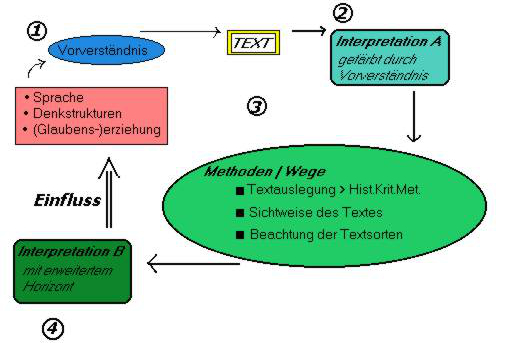
\includegraphics[width=0.8\linewidth]{Hermeneutik}
        \caption{Schematisches Schaubild des hermeneutischen Zirkels}\label{Hermeneutik}
    \end{center}
\end{figure}
\\Des weiteren muss man beachten, dass die Bibel im Original in Hebräisch und Altgriechisch geschrieben wurde. Die Bibel wurde also mehrmals übersetzt. So können mehrere Worte übersetzt das gleiche deutsche Wort ergeben, aber eine völlig unterschiedliche Bedeutung haben. Auch wenn die meisten nicht die Bibel in der Originalsprache lesen können, so muss man dies im Hinterkopf behalten, vor allem bei einzelnen kritischen Worten wie ``Hölle''. Ein Fehler, den man machen kann wie im dritten Reich, ist es, die Bibelstellen einzeln zu betrachten und nicht als ganzes in der Bibel. Mit einzelnen Stellen sind Fehlinterpretationen wahrscheinlicher und es können so martialische, ``antichristliche'' Ereignisse legitimiert werden wie die absolutistische Herrschaft von Adolf Hitler. Die effektivste Möglichkeit wäre theoretisch, für jeden Sachverhalt die Bibel von Anfang bis zum Ende zu untersuchen.
Zuletzt kann man die gegeben Stelle metaphorisch oder symbolisch betrachten, da Jesus und Gott mithilfe von Gleichnissen und Metaphern arbeiten. Diese Stellen sind meistens aber -zum Glück- leicht herauszufinden und zu deuten.
\begin{figure}[h]
    \begin{center}
        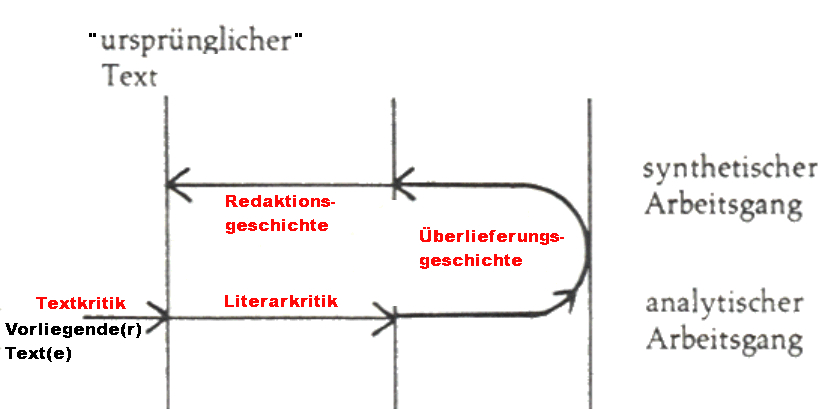
\includegraphics[width=\linewidth]{Historisch_kritische_Methode}
        \caption{Vereinfachtes Schaubild der historisch-kritischen Exegese}\label{HiKrMe}
    \end{center}
\end{figure}
\\Wie muss man also die Bibel verstehen? Es gibt keine Generallösung. Die eine Bibelstellen kann man direkt deuten, die anderen mithilfe von geschichtlichen Wissen, die andere mithilfe von verschiedenen Übersetzungen und die anderen metaphorisch. Und dann gibt es Stellen, die man auf alle Arten und Weisen deuten kann. Deshalb gibt es verschiedene Methoden wie die historisch-kritische Exegese (siehe Abb.\ \ref{HiKrMe}) oder den hermeneutischen Zirkel. Das einzige, was immer zutrifft, ist, dass man die Bibel immer als ganzes betrachten muss. Wann man wie was verstehen muss, muss man im jeden Fall einzeln abwägen. Dies macht das Bibelverstehen auch so schwierig und kontrovers. Zum Glück, jedoch nicht in allen Fällen und unter allen Umständen. Leider.



\chapter{Fazit}
Wichtig zu erwähnen ist, dass vieles hier auf Spekulationen, Hypothesen und Theorien beruht. Es gibt zwar Sachverhalte, die fundiert darzustellen sind, aber vieles fußt auf unbewiesenes und ist sogar heutzutage umstritten. Zweifelsfrei fließt neben der Wissenschaft auch sehr viel Glauben in dieses Fazit. Aber als ganzes bilden sie einen plausiblen Beweis, der nahezu alle meine Zweifel beseitigen kann.
\\
Die Bibel ist einzigartig. Sie ist zweifellos historisch Zuverlässig und es werden immer mehr archäologischen Funde bekannt, die dies immer mehr stützen. Die Bibel wurde nicht gravierend über die Zeit verfälscht und die Bibel, wie wir sie heute vorliegen haben, unterscheidet sich kaum von der damaligen Urfassung. Als Geschichtsschreibung und Geschichtswerk ist sie tadellos. Wenn man die Bibel anzweifelt, dann zweifelt man die Geschichte seit dem Mittelalter an und die gesamte Geschichtsschreibung.
\\~\\
Das Alte Testament ist von Gott inspiriert. In Anbetracht dessen, dass viele Menschen Gottes nahezu deckungsgleich schreiben, beweist dies nahezu. Die einzige Ausnahme sind die Vorschriften, Bräuche und Gesetzte der Priester oder anderer Machthaber und deren Legitimität. Diese wurden (bewusst oder unbewusst) durch die ``Machtgeilheit'' der Priester beeinflusst und sind so kritisch zu betrachten. Diese spielen aber zum Glück für das Christentum kaum eine Rolle und wurden im neuen Testament reformiert. Selbst die fragwürdigen Prophetien sind immer eingetreten und -wenn auch nur historisch gesehen- überliefert. Einzig in die Regel- und Ritualgebung sind menschliche Einflüsse zu verzeichnen, welche jedoch durch Jesus reformiert wurden.
\\~\\
Das Neue Testament ist auch von Gott inspiriert. Die Untersuchung der Autoren lässt darauf schließen, dass alle treue Nachfolger von Jesus und Gott waren. Widersprüche sind kaum zu finden und haben keinen großen Einfluss auf die Auslegung. Viele berichten indirekt oder direkt aus den Überlieferungen von Augenzeugen. Bei allen lassen sich -wenn auch nur hypothetisch- Motivationen nachweisen, welche auf eine göttliche Inspiration fußen und bei allen war der Zweck der Schrift einzig und allein die Verbreiten der Lehren Jesu und zwar so, wie er sie gelehrt hat oder wie er sie auslegen würde. Einzig die Offenbarung des Johannes muss kritisch angesehen werden. Zwar wurden die früheren Propheten des Alten Testaments als von Gott inspiriert eingestuft, jedoch ist bei diesen die Prophetie eingetreten, was bei der Offenbarung nicht behauptet werden kann. Erst wenn wir uns in der Endzeit und der Apokalypse befinden, können wir sicher sein, dass die Offenbarung göttlich inspiriert ist.
\\~\\
Gestützt durch Wissenschaft, plausiblen Theorien und Glauben kann ich reines Gewissens sagen: Die Bibel als Ganzes ist die heilige Schrift. Sie ist das Wort Gottes.
\chapter{Anmerkungen}
\section{Bibelkritik ist erlaubt}
Die Bibel wird unter Fachkreisen als Gotteswort in Menschenwort bezeichnet. Gotteswort, weil der Inhalt vom heiligen Geist gegeben wurden und Menschenwort, da der Verfasser diese empfangen, auslegen und verbreiten musste. Gottes Wort ist unfehlbar, aber wie die Fehlbarkeit des Menschen ist das Menschenwort selber fehlbar. Der simple Sachverhalt, dass Gottes Wort erst von einen Menschen empfangen, mit dessen Verstand ausgelegt, interpretiert, verfasst und einer teilweise langen Redaktion durchlaufen muss, erhöht die Wahrscheinlichkeit für Fehler. Deshalb ist Bibelkritik durchaus erlaubt, da das Menschenwort fehlbar ist und Gotteswort -im Gegensatz z.B. zum Koran- nicht wortwörtlich diktiert wurde.
\\~\\
Dies sieht man auch sehr gut in den Konflikten innerhalb der Bibel. Mose predigte noch, dass Juden keine nicht-jüdische Ehepartner haben dürfen. Bei einen Verstoß müssten diese und die zwei folgenden Generationen aus der jüdischen Gemeinde ausgeschlossen werden. David hatte nicht-jüdische Großeltern und war nebenbei noch der König des damaligen Israels. Von der Ausschluss aus der Gemeinde fehlt jede Spur. Das Alte Testament entstand in  1000 Jahren und das merkt man ihm an. Dies hat nicht zur Konsequenz, dass die ganze Bibel eine Lüge ist, vielmehr ist es eine Aufforderung, die Bibel kritisch zu lesen, aber auch selbstkritisch. Die Bibel ist Gottes lebendiges Wort, sodass die 3000 Jahre alten Worte noch heute Aktualität haben und neu ausgelegt werden müssen. Deshalb müssen wir die Bibel selbstkritisch lesen, sodass das lebendige Wort Gottes auch unser leben verändern kann und nicht zu einen toten Wort wird.

\section{Definition von Inspiration}
Während dieser Untersuchung wurde zu häuft von der göttlichen Inspiration geredet. Der Begriff ist ziemlich selbsterklärend. Die göttliche Inspiration meint, ob ein Autor wirklich sein Wissen durch und mit den heiligen Geist niedergeschrieben hat oder ob alles  lediglich seiner Fantasie entspringt. Doch letztendlich kann der Begriff doch nicht so einfach behandelt werden, wie er es anmuten lässt.
\\~\\
Welche Person als wirklich inspiriert zu betrachten ist und wodurch sich die göttliche Inspiration auszeichnen lässt ist eine sehr umstrittene Kernfrage der Bibelwissenschaften. Unterschieden wir in vielerlei Hinsicht. Es gibt die Modelle der Personen-, der Real- und der Ganzinspiration und alle bergen sie den Anspruch, die Inspiration eines Verfassers wissenschaftlich belegen zu können. Doch schlussendlich treffen sie auf dasselbe Problem: Eine solche Inspiration kann man nicht beweisen, da man sich in einen Bereich befindet, der sich außerhalb der empirisch erfassbaren Größen der Wissenschaft bewegt und so nicht eindeutig bewiesen werden kann.
\\~\\
Es kann nur unter personenspezifischen Grundannahmen beurteilt werden, d.h.\ man erachtet eine Person als göttlich inspiriert und leitet daraus die Charakteristika  einer solchen Inspiration ab, die man dann weiter übertragen kann. Hat man diese auf eine anderen Verfasser übertragen und erachtet ihn so auch als göttlich inspiriert, kann man wiederum aus seiner Schrift Charakteristika ableiten und weiter übertragen. Daraus entsteht dann ein Modell, welches unter bestimmten Grundannahmen beruht. Die Grundannahme bestimmt das ganze Modell. Das Glück des Christentum ist, dass alle an Jesus Christus als Sohn Gottes glauben und z.B. an Paulus als der erste große Theologe des Christentums, den Christus selbst begegnet ist. Somit sind einheitlich anerkannte Autoritäten vorhanden, aus denen man eigener maßen allgemein anerkannte Grundannahmen ableiten kann. Ohne solcher glücklichen Sachverhalte würden sich Modelle in noch größeren Dimensionen unterscheiden.
\\~\\
Des weiteren spielt das Bibelverständnis eine Rolle. Ein Fundamentalist wird kaum die göttliche Inspiration anzweifeln. Ein Historisch-kritischer Theologe jedoch schon. Der eine sieht die Bibel als Gottgegebenes Wort, der andere als eine Schrift von vielen Schriften. In dieser Arbeit wird die Bibel als Zeugenberichte verschiedener Personen betrachtet, die ihre Erfahrungen, Erlebnisse oder Offenbarungen niedergeschrieben haben. So ist jedes Buch nicht mehr als ein Zeugnis. Die Ausnahme bilden die Evangelien. Dies ist auch ein Bericht von einen Zeugen. Jedoch ist es ein Zeugnis von den Taten und Lehren Jesus. Wer nicht an der Glaubwürdigkeit der Evangelien zweifelt und Jesus als Gottes Menschwerdung sieht, für den hat der Inhalt einen absoluten Wahrheitsanspruch.
\\~\\
Aus diesen Gruüden wurde auf ein komplexeres Modell verzichtet. Die göttliche Inspiration wurde jeweils von der Motivation, dem Glaubensleben und den persönlichen Hintergrund abgeleitet. Letztendlich ist die Frage nach der göttlichen Inspiration eine Glaubensfrage, die sich jeder selber mit Ja oder Nein beantworten muss, unabhängig von den Modellen dritter, die aus deren Präferenzen und Vorstellungen entsprungen sind. Manchmal muss man sich aus seinen komplexen Denken und Ansprüchen raus lösen und auf einfache Fragen und Methodiken zurückbesinnen. Die Frage nach der göttlichen Inspiration ist eine und daher wurden hier nur zwei simple Fragen gestellt: Können Beruf, Motivation und Berufung auf eine göttliche Inspiration hindeuten? und/oder Kann ich den Verfasser genug vertrauen, um seine Schrift als göttlich Inspiriert zu betrachten?

\section{Kanonisierung}
Da der Zweck dieser Überprüfung ist, zu schauen, ob die heutige Bibel glaubwürdig ist und nicht, ob die Bibel in heutiger Form anders aussieht, als sie aussehen sollte, wurde der Aspekt der Kanonisierung nicht explizit angesprochen, obwohl es eine wichtige Rolle in dem Entstehungsprozess der Bibel spielt. Daher gibt es nur ein paar Anmerkungen zur Kanonisierung.
\\~\\
Es gab fünf Richtlinien, nach denen entschieden wurde, ob einen Schrift kanonisch, also zu heiligen Schrift gehörig, sein soll.
\\
1. Ist es autoritativ? --- Kam es von der Hand Gottes?
\\
2. Ist es prophetisch? --- War es von einen Mann Gottes geschrieben?
\\
3. Ist es authentisch? --- Es galt die Einstellung, bei Zweifel diese Frage zu verneinen, um so die Gültigkeit der Beurteilung der kanonischen Bücher sicherstellen zu können.
\\
4. Ist es dynamisch? --- Besaß es die lebenserneuernde Kraft Gottes?
\\
5. Wurde es angenommen, gesammelt, gelesen und gebraucht? Wurde es vom gläubigen Gottesvolk akzeptiert?
\\
Es ist offensichtlich, dass diese Gesichtspunkte sicherstellen sollten, dass eine Schrift göttlich inspiriert und kein Hirngespinste waren bzw.\ sind. Es ist also auch als eine Art Fragenkatalog zur göttlichen Inspiration zu sehen, der um einen kirchenpolitischen Gesichtspunkt (Siehe 5.) erweitert wurde.
\\~\\
Die Kanonisierung des Alten und des neuen Testaments ist ein langwieriger Prozess gewesen, dessen Betrachtung den Rahmen sprengen würde. Wichtig zu wissen ist, dass es bereits eine Entwicklung des Kanons vor den offiziellen Konzilen gab, in dem der Kanon in ähnlicher Form wie heute existierte. Der Vorwurf, dass ein Paar kirchenpolitische Entscheidungsträger willkürlich entschieden hätten, welche Schrift kanonisch ist oder nicht ist unangebracht.
Zudem haben sich genügend kluge Menschen und Denker darüber die Köpfe zerbrochen, welche Schrift denn nun kanonisch sei und welche nicht, sodass man diesen Kanon durch die große Masse an Debatten annehmen kann.

% !TEX root = Mein Credo.tex
\part{Die Lehren von Jesus Christus}
\chapter*{Die Lehren von Jesus Christus}
Da Jesus der Messias war, ist und immer sein wird, von ihn Lehren in Form der Evangelien überliefert sind, sind diese
Lehren bedingungslos als Gottes Botschaft zu deklarieren und daher sind die Lehren von Jesus Christus als erstes grobes
Gitter für den christlichen Glauben zu nehmen. Jesus Christus ist neben Gott selber die höchste kirchliche Autorität.
Seine Botschaft und seine Lehren und dessen Wahrhaftigkeit sind daher unumstritten, wenn auch die Auslegung der Lehren
teils sehr kontrovers sein können.\\

Erste Kernaussagen und Kernthemen können aus dem Leben von Jesus Christus entnommen und bearbeitet werden. Im folgenden
wird chronologisch das Leben von Jesus Christus abgearbeitet und entsprechend der Reihenfolge seine Lehren bearbeitet
und für die alltägliche Anwendung ausgelegt. Bei der Exegese werden gehobenere hermeneutische Methodiken erst zur Hilfe
gezogen, wenn mit einer standardmäßigen Exegese die Auslegung nicht mehr einwandfrei zu bewerkstelligen ist und nur
durch eine Disziplinierung des Herausarbeitens alle wichtigen Aspekte gedeckt werden können. Ansonsten wird bis dato
der Verfassung die Position vertreten, dass das lebendige Wort Gottes am besten auch lebendig, also undiszipliniert und
auf die persönlichen Präferenzen und der aktuellen Situation abhängig, am besten ausgelegt werden kann. Dies ist auch
der Grund, warum die folgende Ausarbeitung nicht für jedermann zutreffen und für ihn einwandfrei nachvollzogen werden
kann, da die Auslegung auf mich zugeschnitten ist. \\

Zu wichtigen Stationen im Leben Jesus gibt es Kirchenfeste. Diese sind Feste der Erinnerung und Mahnung und oft nicht
biblisch. Daher ist nicht das Ziel christliche Feste oder Abschnitte im Kirchenjahr auf ihre durch die Bibel bestätigte
Existenzberechtigung zu hinterfragen, denn die existiert im direkten Sinne nicht. Es geht darum, die Rituale,
Kerngedanken und Leitbilder des jeweiligen Festes zu hinterfragen bzw.\ zu erarbeiten und von veralteten Tradition und
Hintergedanken zu lösen. Es geht darum, die Feste in den modernen Kontext einzufügen und für heutige Zeiten angemessen
zu gestalten.

% !TEX root = Lehren__von_Jesus_Christus.tex
\chapter{Weihnachten}
Bevor das Leben Jesu betrachtet werden kann muss erstmal dessen Geburt bzw.\ dessen kommen betrachtet werden. Zunächst geht es also um Weihnachten und die Zeit davor: Advent. Ziel ist es, herauszuarbeiten, wie Advent und Weihnachten eigentlich gefeiert werden sollte, losgelöst von Traditionen, Erwartungen und Kommerz. 

\section{Advent}\label{sec:Advent}
Verwendete Bibelstellen:
\begin{itemize}
\item Römer 13, 11--14
\item Matthäus 11, 2--6
\item Matthäus 24, 29--31
\item Lukas 21, 25--28
\item Philipper 4, 2--9
\item Offenbarung 22, 6--21
\end{itemize}
Die Geschichte hinter dem Advent ist weit bekannt und wird im Abschnitt\ \ref{sec:Weihnachten}: Weihnachten genauer durchleuchtet. Im Folgenden wird daher nur das nötigste Kontextualisiert und Vorhergegriffen. Die Bibel bietet keine breite Grundlage für den Advent und der Weg vor Weihnachten wird zudem im Lukas- und Matthäusevangelium konträr dargestellt. Desweiteren ist die Reise von Nazareth nach Bethlehem wahrscheinlich frei erfunden. Jedoch ist eine Zeit des Vorbereitens und Wartens auf das eigentliche Ereignis nicht falsch, da in Anbetracht des Weihnachtstresses ein harter Einstieg in Weihnachten viele Gläubige das Fest nicht in seiner vollen Form erleben lässt, da sie direkt hineingeworfen werden. Die Vorbereitungszeit ist daher im Kerngedanken eine gute Idee, auch wenn es nicht direkt auf der Bibel fußt.
\\~\\
Bei der klassischen Adventsdiskussion geht es immer um Unterwegs sein (wenn auch nicht im Sinne von Reisen). Alles ist vor und während der Geburt unterwegs, dies dürfte jeden klar sein, die selbst schon bei der Zeit einer Schwangerschaft dabei waren. Wo ein Weg ist, ist auch ein Ziel. Damals war das Ziel die Geburt des Messias. Doch wenn Advent ein Weg ist, was ist dann heute das Ziel, wenn das damalig Ziel bereits erreicht wurde? Wie sieht der Weg aus? Dies sind die wesentlichen Fragen der Betrachtung.


\subsection{Warten auf den Erlöser}
Wichtig sind die Hintergründe der dortigen Zeit. Das Königreich Israel hatte seinen Zenit schon längst überschritten und ist längst zerfallen. Es wurde von dem Römern besetzt und war eine Provinz, die Steuer entledigen durfte und bedingungslosen Gehorsam leisten musste. Die Folge war große Armut und viel Leid. Eine dunkle Zeit in Israel, mit der sich nicht jeder abfinden wollte. Es gab bereits kleine Rebellengruppen, die sich auflehnten und alle erwarteten den Messias, der sie von dieser Situation (oder besser gesagt: Gefangenschaft) befreien würde. Israel wartete auf seinen Erlöser. Sie waren Gefangen in einen Gefängnis. Ein Gefängnis der Besatzung, gegen des sich Israel zunächst nicht wehren konnte.  
\\~\\
Sie waren gefangen, genauso wie Johannes der Täufer. Er wartet auf den Erlöser, der ihn und sein Volk befreien würde. Genauso wie Johannes und Israel zu ihrer Zeit sind auch wir in unseren eigenen kleinen Gefängnis gefangen. Vielleicht ganz ähnlich wie Johannes an einen Ort, an den wir eigentlich nicht sein wollen. Ein Gefängnis aus Streit zwischen zwei Glaubensgeschwistern wie zwischen Synteche und Evodia, die ursprünglich zusammen für die Botschaft Gottes gekämpft haben. Ein Gefängnis, was wir uns selber erbaut haben durch z.B. ein gestörtes Selbstbild. Genau diese Gefängnisse, aus denen wir innerlich am lautesten schreien und am liebsten ausbrechen würden. Oder wie es Paulus im Römerbrief formuliert: Wir schlafen in einer Finsternis und warten darauf, aufzuwachen. Hierbei sind Mächte oder Lebensweisen gemeint, die schlecht für uns sind und uns von Gott und seinen Vorstellungen abbringen oder mit tiefst dogmatisch befleckten Worten: Sünde.
\\~\\
Aus diesen Schlaf sollen wir erwachen. Laut Paulus sei die Zeit gekommen, daraus aufzuwachen, denn die Rettung ist nah. Wir sollen Jesus als den Erlöser in unseren Leben aufnehmen und nicht um unser leibliches Wohlergehen sorgen. Wir sollen keine unnötigen Feste wie z.B. das Oktoberfest feiern, Alkohol nicht missbrauchen, keine sexuelle Verwerflichkeiten begehen und Streit \& Eifersucht meiden. Wir sollen dieselbe Gesinnung gegenüber den Herrn haben und nicht darüber streiten, wie es Synteche und Evodia machten (Heutzutage: Im ökumenischen Sinne). All dies aus den einzigen Grund: Jesus als unser Erlöser ist nahe und ist gekommen, um uns zu erretten. Johannes Warten im Gefängnis auf seinen Erlöser hat sich also gelohnt. Denn Jesus als der Erlöser ist am kommen.
\\~\\
Heutzutage warten wir auf eine andere Weise auf den Erlöser, dennoch ähnelt es sich. Der Messias ist bereits gekommen und brachte, bringt und wird fortan Erlösung bringen. Dennoch warten wir tagtäglich auf einen Erlöser, der uns aus unseren Schlaf aufweckt und uns aus dem Gefängnis befreit. Wir warten genauso wie Johannes der Täufer oder die Israeliten auf den Erlöser, auch wenn sich die Probleme und die Gefängnisse, in denen wir gefangen sind, geändert haben. Jedoch ist Jesus bereits in unser Leben eingetreten und es liegt an uns, ihn als unseren Erlöser anzunehmen und Erlösung zu finden. Wie es Paulus passend formuliert ``Nein, zieht Jesus Christus, den Herrn, an wie ein neues Kleidungsstück'' (Römer 14, 11--14; Basisbibel).

\subsection{Feiern des Advents im heutigen Kontext}
So gerne man auch den Advent feiern möchte, so sehr ist das Fest auch nicht biblisch. Die Bibel gibt keinen Ablauf und kein Leitbild, an dem man festhalten könnte. Der Advent ist wie so ziemlich alle christlichen Feste ein Menschenwerk, um sich an etwas zu ermahnen, zu erinnern und/oder daran sich zu erfreuen. Da das Fest im Mittelalter und somit in einen anderen Kontext eingeführt wurde, lohnt es sich unter Berücksichtigung unseres heutigen Kontextes diese Zeit des Erwartens in seinen Ritualen, seinen Grundgedanken und in seinen Leitbild neu zu überdenken.  
\\
Im Kern ist der Advent ein Fest, um das kommen des Erlösers vorzubereiten. Oder in anderen Worten: Wir bereiten uns auf Weihnachten vor und auf Jesu wiederkommen in der sogenannten Endzeit. Es ist der Gedanke, dass Jesus kommen wird, um uns zu erretten, ähnlich wie damals die Menschen vor der Geburt Jesu. Der Kerngedanke ist also, auf was bevorstehendes zu warten und uns darauf vorzubereiten. Vorbereiten auf das Weihnachtsfest zur Erinnerung an Jesu Geburt. Vorbereiten auf die Endzeit, in der unsere Welt und Gottes Reich eins werden. Doch wie bereitet man es vor? Wie stellt man sich darauf ein? 

\subsubsection*{Vorbereitung auf Jesus Kommen}
Es klingt erstmal perplex, dass Jesus (oder auch: Der Erlöser) kommen soll. Schließlich ist dies alles schon eingetreten. Dennoch sinnen wir tagtäglich auf Erlösung. Die Große Erlösung, auf die wir uns besinnen können, ist die Endzeit. Wir haben das Versprechen, dass wir zu Gott kommen und Teil seines Reiches werden. Alles Leid, alle Plagen, alle Ungerechtigkeiten und all das, was uns auf Erlösung sinnen lässt, wird sich dort in Luft auflösen. All dies wird keine Rolle mehr spielen. Wir wissen nicht, wann dieser Tag kommen wird. Wir wissen nur, dass er kommen wird und dass wir ihn erkennen werden und dass wir zweifelsfrei dort Jesus erkennen werden, der kommen wird, um uns zu retten.
\\~\\
Doch das Versprechen in die Endzeit ist ein explizites Versprechen für ein Event in der Zukunft. Ein Event, wo wir -genauso wie Israel damals auf seinen Messias gewartet hat- auf das Kommen Jesu warten, ohne zu wissen wann und ob es zu unseren Lebzeiten auf Erden geschehen wird. Genau wie damals werden Leute die Endzeit zu früh sehen, ihr komplette Hoffnung mehr auf das Event als auf Gott selber setzen oder radikalisieren sich an den Gedanken eines frühzeitigen Endes. Im Endeffekt können wir bezogen auf die Endzeit nicht mehr machen als damals: auf Gott vertrauen und demütig warten.
\\ 
Doch diese Botschaft hat auch für die Gegenwart eine elementare Bedeutung. Auch jetzt können wir auf Gottes Versprechen bauen, dass auf schlechte Zeiten gute Zeiten folgen werden. Dass er bei Krisen bei uns ist und uns trägt. Und dass wir, wenn wir vermeintlich am Ende sind, Jesus sehen werden und er kommen wird, um uns zu retten. 
\\~\\
In gewisser Weise kann man auch Weihnachten mit einer Art Endzeit vergleichen. An keinen anderen Feiertag haben mehr Menschen frei als an diesen. Um 18 Uhr am heilig Abend steht das öffentliche Leben still und die Leere der Straßen gleichen einer Apokalypse. Man rückt mehr zusammen, Streit und Feindschaften werden beigelegt (jedenfalls die, die man temporär ablegen kann). Jeder füllt seine Kühlschränke auf und rüstet sich für die Feiertage. Weihnachten kann als ein jährliche Endzeit betrachtet werden, auch wenn sie nicht mit den Ausmaßen der tatsächlichen Endzeit vergleichbar ist. Es können also in einen begrenzten Rahmen Parallelen zur Schilderungen der Endzeit gezogen werden.

\subsubsection*{Vorbereitung auf das Fest}
In unseren modernen Gesellschaft ist es Tradition geworden, sich auf ein Weihnachtsfest des unbedachten Massenkonsums und des unbedachten Liebesschenken vorzubereiten. Die Läden müssen möglichst lang offen haben und möglichst viel Umsatz machen. Jedermann soll seinen Mitmenschen was schenken, um ihn so wertzuschätzen. Eine Idee des Marktes. Das Coca Cola den Weihnachtsmann und somit den Brauch des Schenkens als Liebesbeweis erfunden hat, um damit ein Fest zu schaffen, dass ein Rekordumsatz mit sich bringt, ist wohlbekannt. Nicht die Liebe steckt im unbedachten Massenschenken dahinter, sondern Materialismus, Egoismus und das Bestreben nach Reichtum. Irdische Werte und Bedürfnisse, die vergänglich sind. Sicherlich darf man seinen liebgewonnenen Menschen eine Freude machen, indem man ihnen etwas schenkt. Doch reichen dafür wenig gut ausgewählte und mit Liebe gemachte Geschenke. Die Suche nach diesen Bedarf natürlich einen Zeit- und Arbeitsaufwand, doch darf dieser nicht die Adventszeit noch dein Leben zu sehr bestimmen. Hinter dem Weihnachtsfest steckt eine anderer Gedanke und dieser Bedarf keiner großer Vorbereitung. Man muss lediglich den anderen das geben, wovon man selbst zu viel hat.
\\
Für viele heißt es, dass man die Menschen um sich scharen soll, die man liebgewonnen hat, um mit ihnen ein schönes Fest der Liebe zu feiern und nicht das Fest der Geschenke. Dies Bedarf lediglich einen organisatorischen Aufwand und einen geringen Arbeitsaufwand am Fest selber (je nachdem, wie ausgeschmückt man es feiert). Das Fest der Liebe, die aus der Gnade Jesus Christi resultiert, bedarf keinen aufwändig gemachten und teuren Essens. Es bedarf keiner teuren Geschenke. Es bedarf nur der liebevollen Gemeinschaft und für dieses bedarf es nur ein einziges und heutzutage wertvollste Geschenk: Zeit. Nicht die Zeit, in der man 100 Personen mit ihren Festen aus einen Zwang abklappert und jeder Person nur eine Stunde gibt. Es bedarf die Zeit, die man freiwillig in den Maße investiert, wie jeder sie braucht. 
\\~\\
\textbf{Freiwillig}, \textbf{wahre Liebe} und \textbf{Gemeinsam}: Das sind die drei Worte, die das Fest beschreiben.\ \textbf{\textit{Freiwillig}}, weil es nur dann ein Fest der wahren Liebe sein kann, wenn jeder aus freien Stücken da ist und deswegen seine Zeit (und sein Geld) darin investiert. Eine solche wahre Liebe kann nur unter Freiheit bestehen.\ \textbf{\textit{Wahre Liebe}}, weil wir uns an diesen Fest auf Jesus und seine dargebrachte Gnade besinnen, durch die wir Gott in seiner Dreieinigkeit und unsere Mitmenschen erst richtig Lieben können. Und schlussendlich \textbf{\textit{Gemeinsam}}, weil man seine Mitmenschen und Gott nur dann Lieben kann, wenn man seine Zeit gemeinsam mit ihnen verbringen kann. Alles andere kann keine wahre Liebe sein.
\\~\\
Damals bei der Geburt Jesu scharten sich auch viele Menschen um das Kind. Niemand fühlte sich gezwungen, Jesus etwas zu schenken, auch wenn sie vielleicht selber nichts hatten. Sie gaben nur das, was sie in Überfluss hatten. Bei den heiligen drei Königen dürften dies auch wertvolle Sachgaben gewesen sein, da sie wohlhabend waren. Die Hirten dagegen brachten nur ihre Hoffnung. Man soll nur das geben, was man selbst im Überfluss hat oder wo man selbst nicht Not leidet und bei den meisten dürfte das bei den Feiertagen ihre Liebe, Zeit und Gemeinschaft sein. 
\\~\\
\textit{Wenn der gute Wille da ist, ist jeder willkommen mit dem, was er hat und man fragt nicht nach dem, was er nicht hat. Denn es geht nicht darum, dass ihr in Not geratet, indem ihr anderen helft, es geht um einen Ausgleich. Im Augenblick soll euer Überfluss ihren Mangel abhelfen, damit auch ihr Überfluss einmal euren Mangel abhilft.\\ 1. Korinther 8, 12 ff.}

\subsubsection*{Aus eigene Gefängnissen ausbrechen}
Neben den Gedanke des Vorbereitens auf das Kommen Jesu ist wie bereits ausgearbeitet auch ein Kerngedanke von Weihnachten das Warten auf Erlösung. Das Ausbrechen aus den eigenen Gefängnis mithilfe von unsern allmächtigen und barmherzigen Vater in Form von Jesu Christus. Wie so ziemlich alle Lehren von Jesus Christus sind diese auf den Alltag und nicht nur auf ein Fest bezogen und sollten tagtäglich gelebt werden. Jedoch kann es nicht schaden , v.a im Anbetracht der Trägheit des Menschen, sich eine Zeit mit einer Sache genauer und intensiver zu beschäftigen und so jährlich aus den Trott auszubrechen, in den man sich schnell verfängt. Und welches Fest außer Advent eignet sich besser dafür, uns mit unseren eigenen Gefängnissen auseinanderzusetzen und auf den Ausbruch daraus mithilfe von Jesus Christus, der auf die Erde kommen wird, zu hoffen? Auf einen Tag in der Zukunft zu hoffen, in der unser Gefängnis nicht mehr ist?
\\~\\
Für mich persönlich ,um mal aus der Ebene der allgemeinen Lehre auszutreten und es auf mein eigenes Leben zu beziehen, heißt das, zu Advent aus einen eigenen Gefängnis auszubrechen. Sich mit einen tiefer liegenden Problem in seinen eigenen Leben zu beschäftigen und es anzupacken. Für Heilung zu beten und mit unseren Vater darüber im tiefen Gespräch sein. Im Gegensatz zum Fasten geht es hier nicht nur darum, Sachen die einen nicht gut zu tun aus seinen Leben zu entfernen oder auf etwas verzichten. Im Gegenteil, es geht auch um Sachen, die wir bereits machen und nicht schlecht sind, aber die für uns persönlich zu kurz kommen, zu intensivieren. Man kann z.B. Sport machen, was nichts schlechtes ist, aber mit dessen Regelmäßigkeit man (noch) nicht zufrieden ist. Auch ist im Gegensatz zum Fasten hier das Ziel eine nachhaltige Veränderung.
\\~\\
Dabei dient folgende Struktur -angelehnt an das Kommen Jesu- als Vorstellung:
\begin{enumerate}
\item \textbf{Das kommen wir angekündigt}: Zum Anfang des Advent sollte klar sein, welchen Gefängnis man sich widmen will. Es braucht keine Struktur, kein Plan, keine Methodik. Es bedarf lediglich einen Ziel
\item \textbf{Das kommen Jesu wird mit der Schwangerschaft von Maria konkret}: In der ersten Adventswoche soll mit tiefen Fokus auf Gebet und Stille Zeit ein Plan gefasst werden. Eine Analyse des Problems und wo man aktiv werden muss oder Gott uns sagt, dass wir aktiv werden sollten
\item \textbf{Auf den Weg gehen nach Bethlehem}: In der zweiten und dritten Adventswoche soll der Weg folgen. Das heißt ganz konkret den Plan umsetzen, den man sich in der ersten Adventswoche zusammen mit Gott erarbeitet hat.
\item \textbf{Ankommen in Bethlehem und erkennen, dass Jesus die Welt dauerhaft ändern wird}: Die letzte Woche soll dazu dienen, einerseits langsam sich Richtung Weihnachten zu orientieren, andererseits bewusst zu machen, dass die ersten drei Adventswochen wie bei der Reise von Maria und Josef nur der Anfang der Geschichte waren. Jetzt sollte man sich Gedanken machen, wie man aus den Gefängnis draußen bleibt und nicht zurück wandert. Konkret heißt dies, Routinen zu entwerfen, die einen dauerhaft helfen und Kontrollinstanzen zu finden, in denen man reflektieren kann, ob man sich noch auf den richtigen Weg befindet.
\item \textbf{Jesus rettet die Welt für immer}: Irgendwann wird sich (hoffentlich) der Zeitpunkt einstellen, ab den man weiß, dass man es dauerhaft geschafft hat, aus seinen Gefängnis auszubrechen. Jetzt kann man seine Routinen, sofern sie nicht mehr erforderlich sind, ablegen und die Kontrollinstanzen, die man sich selbst geschafft hat, abschaffen.
\end{enumerate}
Diese Struktur ist für mich persönlich als Leitfaden entstanden. Es kann von jeden adaptiert werden, sollen aber keinen Anspruch für die Allgemeinheit haben. Außerdem soll es nur eine grobe Struktur geben, welche sich je nach Problemstellung oder Lebenslage anpassen kann z.B. wie lange eine Phase geht.

\subsection{Fazit}
Advent ist eine Zeit des Unterwegs sein. Das Ziel ist das Weihnachtsfest, die Wiederkunft Jesu in der sogenannten Endzeit und die Erlösung bzw.\ das Ausbrechen aus den eigenen Gefängnissen. Der Weg zeichnet sich (in Reihenfolge der Aufzählung der Ziele) -in meinen persönlichen Fall- durch das Ausbrechen aus einem eigenen Gefängnisses aus. Ein weiterer Weg ist die Vorbereitung von Weihnachten selber, wobei man darauf achten sollte, nur das zu schenken, wovon man selbst im Überfluss hat und das Fest so zu gestalten, sodass kein Zwang entsteht, sodass wahre anstatt vorgegaukelter Liebe in Vordergrund steht und es ein Fest der Gemeinschaft ist. Der letzte Weg zur Endzeit zeichnet sich nicht besonders aus. Zwar hat Weihnachten selber an manchen Stellen endzeitlichen Charakter, doch außerhalb einer inhaltlichen Auseinandersetzung gibt es keinen richtigen Weg, sondern nur ein Versprechen Gottes und eine dauerhafte Einstellung des Gläubigen. 

\newpage
\section{Weihnachten}\label{sec:Weihnachten}
Verwendete Bibelstellen:
\begin{itemize}
\item Lukas 1--2
\item Matthäus 1--2
\item Johannes 1, 1--18
\end{itemize}

\subsection{Kontextualisierung}
Bereits beim Abschnitt\ \ref{sec:Advent}: Advent wurde ein wenig auf den damaligen Kontext um die Zeit von Jesu Geburt eingegangen. Jetzt soll der Kontext genauer betrachtet werden. Als erstes ist die römische Besatzung zu betrachten. Die politischen und wirtschaftlichen Strukturen des römischen Reiches sind (im überschaubaren) Sinne ähnlich zu den heutigen. Das römische Reich kann als ein antikes Modell einer globalisierten Welt verstanden werden. Das politische Geschehen wurde in den wichtigen Entscheidungen zentral in Rom von reichen und/oder einflussreichen Politikern bestimmt und tagespolitische Entscheidungen bzw. Verwaltungen dezentral von eingesetzten Statthaltern bestimmt, die Rom gegenüber zu Loyalität verpflichtet waren, dafür aber auch einbezogen wurden in den Reichtum und Politik. Dies erklärt auch die Nähe von den Hohepriestern (und damit den Sadduzäern) als auch den politischen Machthabern im damaligen Israel zu Rom und das Vorgehen gegen Jesus (und andere Gegner Roms), wenn Rom öffentlich angefeindet wurde oder ein Aufstand angezettelt werden sollte.
\\
Das römische Reich expandierte durch militärische Feldzüge und dies sehr erfolgreich. In eroberten Gebieten wurde den dort ansässigen Machthabern und religiösen Führer Partizipation und Reichtum angeboten, solange sie Rom treu ergeben blieben und ``nach ihren Willen tanzten''. Auch wurde die dortige Infrastruktur gestärkt inform von Straßen, Viadukten o.ä., solange sie Rom Vorteile erbrachten. Die dadurch entstehenden hohen Kosten und die Kosten des Militärs mussten finanziert werden.
\\~\\
Das wirtschaftliche System beruhte auf militärische Expansion. Nach Eroberung wurden die Reichtümer (auch religiöser Natur) geplündert und an Rom weitergegeben. Außerdem gab es ein ausgeklügeltes Steuer- und Abgabensystem. Je näher ein Standort an den Machtzentren des römischen Reichs lagen, desto mehr wurde durch Sozialmaßnahmen versucht, die Bevölkerung bei Laune zu halten. Befand man sich aber außerhalb dieser Zentren, dann waren die Abgaben erbarmungslos und die Bevölkerung musste um ihr Überleben kämpfen. Auch gab es schon damals in Rom Geschäfte mit Spekulationen auf Silber o.ä., was Auswirkungen auf den Wert eines Gutes in eines der Provinzen haben konnte.    
\\~\\
Israel zählte zu den großen Verlieren im römischen Reich. Zusätzlich wurde das Land schon vor den Römern von z.B. den Griechen, die auch nach ihrer Herrschaft noch einen sogenannten hellenistischen Einfluss hinterließen, und anderen Nationen und deren Eroberungsfeldzüge geplagt und zugrunde gerichtet. Viele Juden mussten sogar fliehen und lebten in einer Diaspora. Für Israel hatten die Zustände um die Geburt und das Wirken Jesu endzeitliche Zustände. Dies erklärt auch die Weltansicht einer bösen Welt und einer nahestenden Endzeit und Wiederkunft des Messias, auch nach Jesu Tod hinaus in den Urgemeinden. Gerade diese Zustände riefen viele Aufstände, radikale Bewegungen und Reformbewegungen auf den Plan, einige angeführt von Gläubigen mit den Anspruch, der Messias zu sein. Jesus war also nicht der erste, der behauptete Gottes Sohn zu sein oder der den Glauben reformieren wollte.

\subsection*{Die Evangelien}
Das Evangelium nach Lukas versteht sich nicht als historisch im heutigen Sinne (sondern im damaligen Sinne), aber er versuchte, die Geschichte Jesu in die damaligen politischen und gesellschaftlichen Geschehen einzuordnen, auch wenn ihn dabei ein paar Fehler unterlaufen sind. Der Bericht nach Lukas kann also am ehesten in einen begrenzten Rahmen als ``historischer'' angesehen werden, hat aber keinen Anspruch, eine faktische Historie darzustellen.
\\~\\
Das Evangelium nach Matthäus stellt gewisse jüdische Gruppen negativ dar. Daher ist anzunehmen, dass er von einer jüdischen Gemeinschaft ausgeschlossen wurde. Daher wird in Teilen des Matthäusevangeliums der Konflikt zwischen den ersten Judenchristen und Juden deutlich. Der Fokus liegt darin, Jesus als den Messias darzustellen und daher bezieht er sich auch auf Prophetien des alten Testamentes und er grenzt sich von den ``alten'' Judentum ab. Daher ist kritisch zu betrachten, ob diese Prophetien wirklich geschehen sind oder ob Matthäus, für damalige Verhältnisse in legitimer Weise, einige Sachen zurechtgerückt hat, sodass sich die Prophetien erfüllen.
\\~\\
Es ist anzunehmen, dass Matthäus und Lukas jeweils das andere Werk nicht kannten, was die Unterschiede in der Kindheitsgeschichte Jesu erklärt. Aufgrund der damaligen geographischen Einschränkungen und unterschiedlichen Quellmaterial kann nicht aus den Bibeltext heraus geklärt werden, welche Überlieferung historisch korrekter ist, jedoch haben die Schriften sowieso keinen historischen Anspruch im heutigen Sinne und es muss entschieden werden, wie wichtig korrekte historische Fakten für den Sinn des Weihnachtsfestes sind.
\\~\\
Die Apokryphen hatten auch einen nennenswerten Einfluss auf das heutige Bild von Weihnachten. Der Ochse und der Esel wurden aus den Apokryphen überliefert. Aufgrund der teilweise brüchigen Überlieferung sowie Unstimmigkeiten bei der Inspirationsfrage als auch späte Verfassungsdaten von bis zu 600 n.Chr.\ werden diese nicht mit einbezogen in die Betrachtung.
\\~\\
Da sowohl Lukas als auch Matthäus keinen vordergründigen Anspruch auf korrekte Historizität haben, soll der Kindheitsbericht nicht als historisches Ereignis, sondern als theologische Grundlage für die Evangelien verstanden werden. Da aber Markus keine Kindheitsgeschichte enthält und dies das einzig gemeinsame Geschichtsgut von Lukas und Matthäus ist, aber beide nicht die Evangelien der anderen kannten, ist anzunehmen, dass es sich bei den Gemeinsamkeiten durchaus um Ereignisse handeln kann, die durchaus stattgefunden und sich mündlich bis zu den beiden getrennt herangetragen haben können. Jedoch sollten nicht alle Inhalte der Kindheitsgeschichten als wahre Ereignisse interpretiert werden. Um den Untergang Pompejis gab es auch Sagen und Legenden, aber die Stadt hat wirklich existiert und sie ist wissenschaftlich belegt durch einen Vulkanausbruch zerstört werden. Wenn also beide Geschichten übereinstimmen, kann durchaus eine gewissen Historizität des Ereignisses in Betracht gezogen werden, in Details und Unterschieden jedoch kann es sich um, für damals in den Religionen nicht unüblichen, theologischen Stilmittel handeln, die etwas betonen sollen.

\subsection{Engelserscheinungen von den Eltern von Jesus und Johannes den Täufer}
Engel sind göttliche Wesen, die über den Menschen stehen und Gottes Angesicht gesehen haben. Dieser göttliche Anspruch stärkt die theologische Botschaft, die Lukas und Matthäus zu vermitteln versuchen. Die Existenz von Engeln kann wissenschaftlich nicht bewiesen noch widerlegt werden. Die Existenz wird als widerlegt angenommen und die Engel als Metapher für die guten Wesenszüge von Gott angenommen (siehe \ref{sec:Teufel}). Jedoch kann man Aussagen zu deren Botschaft treffen. Da die Engel in einen klassischen alttestamentlichen Verkündigungsschema reden, ist anzunehmen, dass es sich bei den Engeln um theologische Stilmittel handelt und nicht um historische Ereignisse oder dass der Sinn in einen neuen rhetorischen Rahmen gepackt wurde. Wahrscheinlich ist letzteres Wahrscheinlicher, da sich letzten Endes die Urgemeinde, von der Maria ein Teil war, dies nicht angezweifelt hat und die Verkündigung auch erfüllt wurde. Jedoch sind aus meiner Sicht beide Ansichtsmöglichkeiten plausibel und es gibt nicht die eine Wahrheit. Die Engel bestätigen also den Auftrag sowohl von Johannes den Täufer als auch von Jesus sowie deren Rollen.
\\~\\
Lukas und Matthäus geben Jesus und Johannes Familie einen göttlichen Stammbaum, die  auf das Königsgeschlecht Davids und auf Aaron zurückgehen. Es ist unwichtig, ob diese Abstammung biographischer Art ist. Zu einen gab es damals ein anderes Verständnis von Genealogie (man betrachte den Kult um Heidenkönige als Gottessöhne heidnischer Götter, obwohl sie offensichtlich biologisch von irdischen Leben abstammen) und zu anderen ist hierbei die theologische Genealogie wichtig. Gott erwählte Israel als sein Volk, Moses als sein Prophet und Aaron als seinen Hohepriester. Diese salbten David zum König, der durch Gott bestätigt und bestraft wurde, als dieser sich von ihn abgewandt hatte. Hierauf folgt auf einer Zeit der Verdammung Jesus als der Nachfolger Davids als nächster großer König für die Ewigkeit und Johannes als der Nachfolger Elias soll sein Kommen vorbereiten. Dieser irdische (horizontale) Stammbaum wird hierbei bei Jesus durch Gott von oben (vertikale) durchschnitten. Die Zeit der irdischen Könige ist vorüber und der letzte König kommt für die Ewigkeit und ist kein anderer als Gottes Sohn selber. Der universale Anspruch wird bei Matthäus betont durch die Erwähnung des ``Buches der Abstammung'', das zuletzt bei der Schöpfungsgeschichte der gesamten Menschheit erwähnt wurde und somit zeigt, dass es sich um den König der Menschheit handle. Ebenso zeugt die Abstammung von Abraham davon, dass Jesus Anspruch weltweit gilt, da Abraham ebenso für alle Völker berufen wurde. Dieser Beweis durch eine Abstammung war Matthäus so wichtig, dass er den Stammbaum mit einer ``heiligen Mathematik'' versah, sodass nicht an diesen gezweifelt werden dürfe. Jedoch bedeutet dies nicht, dass eine Abstammung Jesu von David nicht existiert, sondern dass man es mittlerweile einfach nicht mehr sagen kann.
\\~\\
Der universale Geltungsanspruch wird auch durch die Wahl der Herkunft von Jesus unterstrichen. Jesus stammt aus Nazareth, ein Ort niedriger Bedeutung und der gemischten Völker. Jesus wird nicht im Tempel oder im Allerheiligsten verortet, die Orte die dem Allerheiligsten und nur Gott vorbehalten blieben, sondern einen Ort, wo jeder sein darf. Die einzige Verbindung zum Königtum bleibt also bei der Abstammung. Dies bestätigt das Alte und zeigt eindeutig, dass eine neue Zeit anbricht, wobei das Alte nicht aufgehoben wird, sondern eine Verheißung zusätzlich erfüllt wird. Auch zeigt dies, wie tief sich Gott begibt. Er stammt aus einen Dorf, das in Israel religiös als auch wirtschaftlich nahezu komplett unbedeutend war. Er stammt aus einen Dorf, wo jedermann als Letztes nach ihn gesucht hätte.

\subsection{Verheißung auf Erlösung}
Mit der Wahl der Eltern von Johannes liefert die Verheißung direkt Erlösung bzw.\ den Ausbruch aus einem Gefängnis (siehe Advent): Elisabeth  wird erlöst aus den Schicksal der Kinderlosigkeit. Dies war zur damaligen Zeit wirklich ein Gefängnis, da unfruchtbare Frauen als von Gott bestrafte galten und daher in der jüdischen Gesellschaft sehr diskriminiert wurden. Die Berichte erwähnen ihr Frommes leben. Dies zeigt: Die Eltern von Johannes litten zu Unrecht und hatten das ``Recht nach Erlösung'', die Gott ihnen zukommen ließ.
\\~\\
Eine weitere Erlösung wird durch Lukas Einordnung der Geburtsgeschichte in die Zeit der römischen Herrschaft durch Herodes angedeutet. Lukas stellt Jesus als den Erlöser der römischen Herrschaft entgegen. Jesus ist der Erlöser, der von den römischen Reich verfolgt und gekreuzigt wird und damit vermeintlich verliert, jedoch in der Auferstehung den endgültigen Sieg davon trägt.
\\ 
Auch bringt Gott den Eltern Erlösung, bevor sie wissen dass sie in eine  Gefängnis sind. Er erklärt Joseph die Geisteszeugung und verhindert so die Missgunst des Volkes gegenüber Maria und Joseph. Gleiches gilt für die Eltern des Johannes. 
\\~\\
Das Bedürfnis nach Erlösung für das Volk wird v.a.\ bei Matthäus, aber auch bei Lukas wirkungsvoll demonstriert. Beide verarbeiteten das Leid durch die römische Herrschaft in nicht historisch fundierten Geschichten wie dem Kindermord in Bethlehem und die Flucht der Jesusfamilie nach Ägypten. Auch die Volkszählung war ein Zeichen der Unterdrückung. Auch wenn diese Geschichten nur ein ``erfundenes Werk zur Fundierung der theologischen Botschaft'' waren, ist der Kern der römische Unterdrückung dahinter war. Auch wenn nicht unschuldige Säuglinge in Bethlehem getötet wurden, wurden es andere tatsächlich schon. Auch wenn die Familie nicht fliehen musste, wurden andere Israeliten aus ihrer Heimat vertrieben oder mussten fliehen (und Jesus meidete auch gewisse römische Machtzentren auf seiner Reise bis zu seiner Einreise in Jerusalem). Auch wenn es keine Volkszählung gab, gab es später einen Zensus in Judäa nach der Absetzung des Sohnes des Herodes, dass genauso ein Zeichen der Unterdrückung war und für viele eine weitere steuerliche Belastung und die Gefährdung der Lebensgrundlage darstellte. Dem gegenüber wird Jesus in Form des Kindes gestellt, dass konträr gegen Kaiser Augustus steht. Nicht als reicher, mächtiger Feldherr, sonder als friedlicher, armer und politisch unbedeutender Wanderprediger, dessen Anspruch hingegen des von Kaiser Augustus universal und gerechtfertigt war und ist. 

\subsection{Geisteszeugung Jesu und doch nur ein Mensch}
Es ist eine tiefe Diskussion, ob im Urtext Maria als junge Frau oder Jungfrau übersetzt werden sollte. Da die Kindheitsgeschichte an jüdischer Tradition anschließt und in dieser eine (biologisch) jungfräuliche Geburt nie eine Rolle spielt und nie vorhergesagt wurde, ist anzunehmen dass es sich bei der Geisteszeugung um keine biologisch gesehene Jungfrauengeburt handle. Außerdem entstammen Lukas und Matthäus einen hellenistischen Einfluss, in dem Jungfrauengeburten durchaus eine Rolle spielten. Die Jungfräulichkeit ist also eher aus den kulturellen Einfluss von Lukas und Matthäus herzuleiten und sollte nicht biologisch gesehen werden. Leider zieht sich diese Vorstellung bis zum heutigen Tage durch und belegt zuviel Platz in der Weihnachtsgeschichte.
\\~\\
Es ist unwichtig, ob der heilige Geist Maria biologisch geschwängert hat. Wichtig ist, dass der heilige Geist Jesus als seinen Gottessohn ausgewählt hat. Gottessohnschaft bedeutet vollkommene Teilhabe an der Macht Gottes und dem vollen Gehorsam Gott gegenüber. Es geht um eine einzigartige Beziehung Gottes zu seinen menschlichen Sohn. Gott wählte hierfür Marias Sohn aus und der heilige Geist erfüllte sie und dadurch Jesus Geist mit seiner vollen Macht und dieser Geist wohnt in den Körper von Jesus. Wie dieser Prozess biologisch stattfand ist unbedeutend und ein anderes Thema, da Jesus Macht von seinen Geist und seiner Seele ausging und nicht von seinen Körper, ein Körper der menschlicher nicht sein konnte.
\\~\\
Wichtig hingegen ist, dass diese nicht biologisch gesehen jungfräuliche Geburt Jesus noch menschlicher Macht. Jesus hatte Geschwister, eine Mutter und somit eine Familie. Dies ist biblisch belegt und kann entgegen den Willen der Verfechter einer jungfräulichen  Geburt nicht widerlegt werden, da ``adelphos'' immer den Blutsbruder meint. Dies stützt noch mehr die Menschwerdung Jesu, der durch und durch Mensch ist. Und somit wurde Gott durch und durch Mensch. Jesus ist zwar von Gott als seinen Sohn auserwählt und komplett mit ihn erfüllt, was ihn auch eine geistliche Macht gab, biologisch unterschied er sich aber nicht von einen gewöhnlichen Mitmenschen.
\\
Ein zu der Zeit gängiges Verständnis einer Sohnschaft (im königlichen Kontext) war in erster Linie ein rechtliches Verständnis und in zweiter Linie erst ein Verständnis der Blutsverwandtschaft. Ein König bestimmte einen fähigen Mann zu seinen Sohn, der ihn in seiner Vollmacht vertrat und zur rechten des Königs saß (siehe Jörg Zink). Analog wurde Jesus von Gott auserwählt und machte ihn so zu seinen Sohn mit einer geistlichen Vollmacht, die ihn das Predigen und die Wunder ermöglichte. Diese Ansicht mag für viele einen Bruch in ihren Glauben darstellen, jedoch kam der Fokus des Begriffes Sohn auf das Biologische erst nach der Verfassung auf und war zu Zeiten der Verfassung nicht so strikt auf Blutsverwandtschaft getrimmt wie heute. 
Jesus ist wie in einen alten Dogma beschrieben ``Sowohl Mensch als auch Gott'' in Form eines bevollmächtigten Stellvertreter Gottes auf Erden mit hierzu befähigter, geistlicher Macht. Dies bringt uns die menschliche Seite von Jesus enorm viel näher, verändert zugegebenerweise jedoch auch z.B. das Verständnis der Trinität im Vergleich zum gängigen Verständnis.
\\~\\
Seine Menschlichkeit wird auch bei Johannes den Täufer klar. Es ist wahrscheinlich, das Jesus sein Schüler war. Wie von den Engeln angekündigt ebnete Johannes Jesus den Weg. Er schuf nicht nur eine Bewegung und Aufmerksamkeit für die Missstände, er bereitete auch Jesus auf seine Aufgabe vor. Es ist nicht eindeutig geklärt, ob sich Johannes selber seinen Schicksal bewusst war und/oder sich als Wegbereiter verstand, jedoch ist dies egal. Er schulte Jesus, den Menschen der selbst noch lernen und sich auf seinen Weg vorbereiten musste. Nicht, weil seine göttliche Seite geschult werden musste, sondern weil seine menschliche Seite auf seine Bestimmung vorbereitet werden und lernen musste, mit der göttlichen Seite umzugehen. Johannes bereitete ihn, wissentlich oder unwissentlich, darauf vor. Dies alles mündet in der Taufe, die Weihnachtsgeschichte von Markus (in seine Augen wurde der Messias bei der Taufe erst richtig geboren) in der der Heilige Geist die Gottessohnschaft bestätigt und ihn auf seine Mission sendet. Jesus ist ab da ``bereit'' und wird von Schüler Johannes zu einen Wanderprediger, der Johannes übertrifft.

\subsection{Bezeugung der Bestimmung Jesu}
Sowohl das Magnifikat Marias (Marias Lobgesang vor Gott) als auch die Reise zu Elisabeth sind wahrscheinlich nicht historisch. Dies ist jedoch nicht wichtig. Das Magnifikat war wohl zu der Verfassung des Lukas-Evangeliums ein weitläufiges Lied der ersten Gemeinde. Das Lied ist ein Zeugnis der Erfahrungen der Anhänger und zeigt die Wirkung Jesu auf die frühchristliche Gemeinschaft. Dass es ein bekanntes Lied war bezeugt den Konsens der Urgemeinde in der theologischen Botschaft des Liedes. Dass sich Lukas zutraut, das Magnifikat in den Mund von Maria zu legen, vor der Lukas offensichtlich viel Respekt hatte, bezeugt die theologisch Wahrheit noch mehr. Das Magnifikat ist die Bezeugung von den Wirken Jesu und dessen Sprengkraft. Das Lukas Maria das Magnifikat in den Mund legt, mindert nichts an der Wahrheit der theologischen Botschaft des Magnifikat, dass unendliches Vertrauen in Gott und die Veränderung der Welt aus den Glauben heraus fordert und bezeugt.
\\ 
Gleiches gilt für die Reise zu Elisabeth. Nur, dass sie nicht stattgefunden hat ändert nichts an der Wahrheit der Botschaft, dass Elisabeth und stellvertretend für sie die ersten Anhänger durch den Heiligen Geist die Begeisterung ihres Kindes sowie Jesus als den Messias erkennen können. Beides sind als Bezeugungen für die Gottessohnschaft Jesu und dessen Wirken zu verstehen. Lukas nimmt hier schon das Ergebnis des Wirken Jesu vorweg. 
\\~\\
Gleiches gilt für die heiligen drei Könige, die als eine Gruppe unbekannter Größe aus ``Magiern'' (also Heiden) in der Bibel dargestellt werden. In Anbetracht des Kontextes wird Herodes sie nicht unbeobachtet ziehen lassen, wenn ein neuer König ihn seine Macht strittig machen soll. Er setzte seine Macht und Spionageapparat für viel weniger ein, dann hätte er ohne Zweifel bei der genannten Überlieferung jeden Schritt penibel verfolgt. Direkt damit im Zusammenhang ist der Kindermord in Bethlehem und die Flucht bzw.\ Verfolgung der Jesusfamilie. In Anbetracht des Kontextes hätte Herodes sicherlich die 10--15 Kinder hinrichten lassen und die Familie gesucht, wenn die Geschichte wahr wäre. Jeder einzelne Aspekt der Geschichte fand nicht statt, jedoch greift dies das Ergebnis Jesu Wirken vorweg: Jesus bringt Menschen aus allen Völkern und ethnischen Hintergründen zu Gott und ist für alle gekommen. Aber wir können viel aus der Geschichte lernen. Sie zeigt, dass nicht nur Vernunft zu Gott führt, denn die Vernunft der Magier hat sie zu ihrer heidnischen Religion geführt. Ihr Vertrauen in ihr Gefühl trieb sie die ganze Reise zu Jesus hin durch alle Widrigkeiten und ließ sie direkt ohne nachzudenken vor Jesus niederfallen. Eine erfundene Geschichte, die jedoch über die Jahrtausende trotzdem mehrmals stattgefunden hat (vgl.\ das Buch/Film ``Der Fall Jesus'').

\subsection{Eine Geburt in Armut, Elend um am Rande der Gesellschaft}
Das Jesus in Bethlehem geboren sein soll, ist historisch fragwürdig. Es kann nicht eindeutig geklärt werden, ob die Geburt nun wirklich in Nazareth oder Bethlehem stattfand, jedoch ist die Volkszählung faktisch nicht der Grund des Aufenthaltes, da 
\begin{itemize}
\item[a)]eine solche Volkszählung nicht sattfand und
\item[b)]der Zensus unter Quirinius im Wohnort vorgenommen wurde, da man dort seine Seer und Abgaben zahlte und Joseph garantiert aufgrund der Opferung von Tauben anstatt von Lamm kein Besitz außerhalb von Nazareth gehabt haben konnte.
\end{itemize}
Auch ist fragwürdig, warum eine hochschwangere Frau eine solche gefährliche und anstrengende Reise unternehmen sollte. Jedoch ist die Historizität des Geburtsortes nicht wichtig. Wie bereits zuvor erörtert dient dies zur Legitimation, dass Jesus der Messias ist. Wahrscheinlich wurde er in Nazareth geboren, jedoch sind die Umstände die Gleichen. Jesus wurde unspektakulär in Armut geboren. Behütet durch seine Familie, aber nicht prunkvoll in einen Palast, wo es alle Welt direkt erfährt. Es war eine ``unbedeutende'' Geburt in die Armut hinein. Joseph durfte aufgrund seiner Armut anstatt eines Lammes zwei Tauben für die Geburt Jesu opfern, was nur Armen gestattet wird. Jesus Leben begann am Rande der Gesellschaft und schon dort wird der Fokus des Wirken Jesu auf die verstoßenen und Verlierer der Gesellschaft deutlich. Natürlich erfüllt dies nicht die Prophetie von Micha, doch ist dies eine Auslegungssache, v.a.\ ob Micha Bethlehem als Geburtsort oder Abstammungsort der Familie meint.
\\
Ob Jesus wirklich von Hirten besucht wurde, kann mittlerweile nicht mehr geklärt werden. Jedoch betont auch dies, dass Gott sich auf die niederste Ebene der Gesellschaft herabließ, sodass Hirten, sowohl sozial als auch religiös angefeindet in der Gesellschaft, die ersten waren, die den Messias sehen durften. Ihr Verhalten ist bemerkenswert. Sie ließen alles auf die Verheißung hin stehen und begegneten Jesus. Sie gingen recht rasch wieder zurück in ihren Alltag und preisten und lobten den Herrn. 
\\~\\
Dass (nicht erfundene) Motiv der Armut Jesu und sein Zugehen auf Randgruppen zieht sich durch die ganze Weihnachtsgeschichte als auch die Evangelien. Gott begab sich von seinen himmlischen Thron so tief in den Dreck, um uns zu erretten. Daher scheint neben der offensichtlichen  Legitimation des Anspruches auf die Gottessohnschaft die Geburt in die Armut, das Elend und dem Rande der Gesellschaft hinein und damit der Fokus der Heilmission Jesu auf diese Gruppen zu sein.

\subsection{Fazit}
Der offensichtliche Kernpunkt ist die Menschwerdung Gottes und somit die Gottessohnschaft. Dabei gab es keine Jungfrauengeburt, sondern eine reine ``geistliche'' Zeugung, bei der Jesus von Gott als seinen Sohn bevollmächtigt und hierfür mit seinen bekannten Fähigkeiten bestückt wird, aber mit keinen biologischen bzw.\ göttlichen Körper. Auch wird schon das Ziel Jesu vorgegriffen: Die Menschheit -und nicht nur das Judentum alleine- zu erlösen und zu befreien (mehr dazu später).
\\~\\
Ein weiterer zentraler Aspekt ist die Geburt in die Armut das Elend der Gesellschaft herein. Die Geburt war nicht pompös, edel oder königlich in aller Öffentlichkeit, sondern ein ``unbedeutendes'' Event, in den die Armen und Verstoßenen als erste und einzige das Jesuskind sehen durften.
\\~\\
Die Reise zu Elisabeth, der Stammbaum, die heiligen drei Könige und der Kindermord in Bethlehem als auch die Flucht fanden wahrscheinlich nicht statt, jedoch stimmt die Botschaft dahinter und wird später im Leben von Jesus Christus bestätigt. Dies sind also Projektionen späterer Ereignisse und dient primär der Legitimation der Gottessohnschaft Jesu. 
\\ 
Generell kann die Kindheitsgeschichte Jesu als Ouvertüren der Evangelien und das Wirken Jesu gesehen werden.

\subsection{Feiern des Weihnachtsfestes im heutigen Kontext}
Das Weihnachtsfest ist ein Menschenwerk und hat keine biblischen Riten o.ä.. Es ist ein Gedenkfest und die inhaltlichen Themen zum darauf Zurückbesinnen können den Fazit entnommen werden. Jedoch kann sicher gesagt werden, dass mit Weihnachten das Kirchenjahr beginnen soll, sofern Jesu Wirken als ein Rahmen für das Kirchenjahr angenommen wird, da Jesu Geburt offensichtlich der Anfang seines Wirkens ist. Abseits dem theologischen Auseinandersetzen und Besinnen kann, was den Rahmen, Rituale und die Strukturen des Festes angeht, folgendes gesagt werden:
\\~\\
Weihnachten sollte genau wie die Geburt damals \textit{kein} pompösen, überzogenes und überhobenes Fest sein. Es sollte sich auf das offensichtliche berufen werden: Das Kind in der Krippe. Das Christuskind war umhüllt von armen Gestalten und Verstoßenen der Gesellschaft. Deshalb sollte zu der Zeit auf die Armen und Ausgestoßene, im Volksmund die ``Verlierer der Gesellschaft'', geschaut werden und reflektieren, wie man diesen ganz aktuell und generell helfen kann. Auch kann man auf die symbolische Armut der Mitmenschen geschaut werden. Wie zuvor beim Punkt Advent erörtert sollte man die Dinge geben, die man selbst im Überfluss hat und wovon ein anderer benötigt, sei es materiell oder immateriell. Und dies kann auch durchaus Geschenke für die materiell Armen geschehen, zu welchen auch so ziemlich alle Kinder gehören, die durch den Reichtum ihrer Eltern beschenkt werden (im wortwörtlichen als auch übertragenen Sinne).
\\~\\
Das Christuskind war umgeben und behütet von seiner Familie, auch später in seiner Kindheit. Das Weihnachtsfest sollte daher ein Fest für und mit der Familie sein, sowohl die Blutsfamilie als auch die geistige Familie. In Verbindung mit zuvor genannten kann man sich auch mit Freunden treffen, die von Ferner kommen und/oder mit denen man (aufgrund der vorherrschenden geographischen Distanz) im Jahr über weniger Zeit verbringt. Dabei sollte die Liebe der Familie zueinander im Vordergrund stehen wie die Liebe von Jesus Eltern zu ihn. Materielle Dinge sowie der Kommerz sollten im Hintergrund rücken und gehören nicht zum christlichen, sondern zum weltlichen Weihnachtsfest, was jedoch nicht heißt, dass es auch in einen begrenzten Rahmen im christlichen Weihnachtsfest Raum finden kann, wenn es den eigentlichen Kernpunkten zugute führt.  
\\~\\
Man kann sich auf auf die Erlösung und das Ziel der Heilmission Jesu berufen, die mit Jesus Christus auf die Erde kommt. Hierzu zählt u.a.\ auch das Kreuz und die Endzeit, jedoch haben diese Themen später im Kirchenjahr auch ihren Platz, weswegen sie nicht zu sehr Platz einnehmen sollten. Wichtiger als der bevorstehende Weg ist immernoch die Geburt bei Weihnachten.

\subsection{Kindheitseschichte}
Die Kindheitsgeschichte von 12-jährigen Jesus gibt es nicht allzuviel neues zur Geburtsgeschichte zu erzählen, bevor wir zur nächsten großen Kapitel (die Taufe) kommen. Der Vollständigkeit halber ein paar Anmerkungen zu diesen Text: Er kommt nur in Lukas vor und ist der einzige Kindheitstext im Kanon. In den ist Jesus sich bereits seiner Gottessohnschaft bewusst, jedoch auch, dass sein Zeit noch nicht gekommen ist und er noch heranwachsen muss.
\\~\\
Hier wird wieder die Dualität zwischen Jesus als Mensch und als Gottes Sohn aufgezeigt. Einerseits muss er als Mensch lernen. Er löchert die Schriftgelehrten mit Fragen und geht danach wieder zurück nach Nazareth, um heranzuwachsen. Die ganze Zeit ist er seiner Familie untergestellt, trotz seiner höchst göttlichen Berufung. Andererseits ist er bevollmächtigt durch Gottes Geist. Er als 12 jähriges Kind hat -was theologische Themen betrifft- eine geradezu übernatürliche Auffassungs- und Deutungsgabe. Er ordnet die Antworten der Schriftgelehrten schnell ein und bietet ihnen Paroli und das als junges Kind. Seine geistliche Vollmacht Gottes befähigt ihn dazu. Es ist so, als würde ein 10 jähriger (die geistliche Entwicklung heutiger Menschen ist unterschiedlich zu damals, weil man heute nicht mehr mit 14 Erwachsen ist und ein Arbeitsleben bestreiten muss usw) mit Professoren an der Uni auf Augenhöhe diskutieren.
% !TEX root = Lehren__von_Jesus_Christus.tex
\chapter{Taufe}
Auf die Geburt und die Jugendgeschichte von Jesus folgt in allen 4 Evangelien die Vorstellung von Johannes den Täufer und dessen Taufrituals, welches sich Jesus anschließend selbst unterwirft. Daher soll als nächstes das Thema Taufe näher betrachtet werden.

\section{Kontextualisierung}
Im alten Testament und somit im alten Judentum spielte das Konzept der Reinheit eine große Rolle. Nach damaligen Verständnis war Reinheit das Gott gemäße und wiederum (kulturelle) Unreinheit ein Zustand, in dem man sich nicht dem Heiligen (z.B. Tempel, Synagogen usw.) nähern durfte. Die Begründung der Reinheitsgesetze waren durchaus komplex, aber nicht komplett theologischer Natur.
\\~\\
Im Hinblick zu der Taufe sind die damit verbundenen Reinigungsriten interessant, durch die bei Unreinheit der Zustand der Reinheit wiederhergestellt werden konnte. So gab es z.B. Mikwen als Ort der regelmäßigen Reinigung. Vermutlich nach der Zerstörung des Tempels wurde sogar ein Mikwenbad nach einer Konversion vorgeschrieben. Es gab aber auch andere Formen der Reinigung, die entweder selbstständig oder durch einen Dritten durchgeführt werden konnten. Am Ende musste die Reinigung von einen Priester bestätigt werden.
\\~\\
Erste Motive der Taufe gab es schon im Alten Testament. Dort wurde Naaman in einen Fluss gewaschen und somit bekehrt. Auch gaben Propheten o.ä.\ schon Konzepte in den Kontext von Moral und Ethik. Auch kündigten Propheten an, dass Gott selbst kommen und die Reinheit wiederherstellen wird. Auch wird Johannes der Täufer als Personifizierung von alttestamentlichen Motiven von Reinheit gesehen.
\\~\\
Wie zu sehen ist, gibt es schon im Alten Testament und somit im Judentum Motive und Riten zur Reinheit, die einen Hintergrund für die christliche Taufe bilden.

\section{Biblische Zeugnisse}
\subsection{Taufe des Johannes}
Über die Taufe des Johannes wird im  Neuen Testament berichtet, beim Markusevangelium ist sie sogar erste Bericht und somit der Anfang der Geschichte nach Markus Vorstellung. Bei Johannes kann die Taufe als die Reinigung der Sünden zum Zeitpunkt der Taufe als auch eschatologisch als Bewahrung vor der bevorstehenden Feuertaufe verstanden werden, wobei in der Urgemeinde die Endzeit schon als sehr nah erwartet wurde. Durch das Heilsgeschehen Jesu am Kreuz ist es ein gängiges theoligsches Bild geworden, dass sich in Jesu kommen sich die Tauferwartung Johannes erfüllt hat und die Partizipation an Jesus Heilsgeschehen nun als Tauferwartung in den Vordergrund gerückt ist. Bei der Taufe des Johannes gab es viele Elemente, von denen einige Bedeutung gewannen und andere an Bedeutung verloren:
\begin{itemize}
	\item Die Taufe geschieht im Jordan, einen Fluss. Im Johannesevangelium wird aber auch z.B. Ainon genannt als Wirkungsort des Johannes, weshalb der Jordan als Ort selber keine große Bedeutung haben wird für das Ritual.
	\item Die Taufe geschieht immer durch einen Täufer, der eine mediatorische Rolle einnimmt: Die Verkündigung und das Ritual selbst gibt nur Gottes Wirken weiter.
	\item Die Taufe war einmalig. Begründet wird dies durch die damalige eschatologische Naherwartung und der geforderten ethischen Neuorientierung, die nur einmalig sein konnte.
	\item Die Taufe hat eine Lebensführung nach der Thora als Konsequenz. Dabei ist die neue Lebensführung als natürlich kommende Konsequenz und nicht als Zwang interpretierbar. Wenn sich der Täufling der Taufe und somit Gott unterwirft, wird er sein Leben nach Gott aus freien Stücken ausrichten. Die Lebensführung nach der Thora kann in heutiger Zeit nicht als eine Lebensführung nach den Alten Testament, sondern nach Jesus Lehren verstanden werden, da er mit Gottes Autorität die Thora Neuinterpretiert und die Lehren reformiert hat.
	\item Die Taufe war kein Inititationsritus. Dennoch war sie ein Unterscheidungsmerkmal, was getaufte und die restliche jüdische Gemeinschaft unterschied.
\end{itemize}

In den Berichten des Matthäusevangelium wehrt Johannes das Taufbegehren Jesu ab: ``Ich habe nötig, von dir getauft zu werden'' (Mt 3,14). Somit wird die Taufe durch Jesus über die Wassertaufe als Ritual gestellt. Im Allgemeinen Fall macht dies kein Unterschied, da der Täufer selbst das Wirken Gottes und somit Jesus Wirken weitergibt, aber für einige Streitfragen wie z.B. die Behandlung von Ungetauften Toten oder ob für Ungetaufte auch die Erlösung Gottes gilt, gibt dies neuen Interpretationsspielraum.
\\~\\
In den Evangelien und zu der Wirkzeit Jesu wird von der Taufe primär im Zusammenhang mit der Johannestaufe berichtet. Auch gibt es Anspielungen und Umstände aus den Berichten, die eine direkte Tauftätigkeit Jesu oder eine indirekte durch seine Jünger vermuten lässt. Somit ist anzunehmen, dass die Taufe als Ritual von Jesus selbst praktiziert und somit akzeptiert wurde, jedoch stellt Jesus nirgendwo die Taufe als Bedingung für z.B. die Heilserlösung dar. Es ist also unbestreitbar, dass die Taufe als kirchliches und biblisch fundamentiertes Ritual/Sakrament interpretiert werden kann, die Verknüpfung der Taufe als fundamentale Bedingung für z.B. Aufnahme in die Gemeinschaft oder Zuspruch von Gottes Erlösung usw.\ kann jedoch nicht trivial beantwortet werden.

\subsection{Übergang der Johannestaufe zur Taufe der Urgemeinde}
Einerseits kann man annehmen, dass die Taufe Jesu als Vorbild übernommen wurde, andererseits -und viel wahrscheinlicher- dass die Jesusanhänger nach Ostern das Bedürfnis hatten, die Zugehörigkeit zum Auferstandenen durch ein von ihnen bekanntes Ritual zu erleben. Dabei war Paulus einer der ersten Theologen, die die Taufe weiter auslegten und als Ritual verbreiteten.
\\~\\
Anmerkung (für alles was Paulus Lehren betrifft): Wichtig zu verstehen ist jedoch, dass Paulus im Grunde auch nur ein Theologe war, der Jesu Worte und Lehren auslegen wollte. Seine Lehren haben zwar durch seine Gotteserfahrung und den Grund, dass seine Briefe im Kanon sind eine erhöhte Aufmerksamkeit, jedoch hat seine Auslegung keineswegs einen Absolutheitsanspruch, diese haben nur Lehren, die auf Jesus bzw. Gott selbst zurückzuführen sind. Dies soll nicht alle Aussagen Paulus infrage stellen, aber seine Lehren dürfen kritisiert und als nicht absolut angenommen werden.
\\~\\
Paulus bzw.\ die Berichte über seine Taufen in der Apostelgeschichte sind die ersten Überlieferung mit einer Taufe auf den Namen Jesu bzw.\ später auf den trinitarischen Namen. Auch tritt mit Paulus die Bedeutung des Taufenden in den Hintergrund, da er im Grunde eh nur ein Vermittler ist und am Ende der Heilige Geist und der Täufling im Vordergrund stehen. Zu der Verfassung des Römerbriefes war die Taufe bekannt, auch wenn sich die Taufrituale untereinander noch unterschieden. Es stand also außer Frage, ob man sich Taufen lassen sollte.
\\~\\
Paulus sieht Taufe und den heiligen Geist sehr eng, jedoch verbindet er damit nicht eine Geistverleihung. Vielmehr verleitet das Wirken des heiligen Geistes den Täufling dazu, seine Schuld abwaschen zu lassen und so vor Gott als gerecht bestehen zu können, oder um es anders zu sagen:
\\
Das Wirken des heiligen Geistes bewegt den Täufling erst zur Taufe und somit zum Leben mit Gott.

\subsection{Deutung der Taufe außerhalb von den echten Paulusbriefen}
Im Kolloserbrief wird die Taufe mit einer Beschneidung aus den alten Judentum verglichen. Der Epheserbrief beschreibt die Taufe als Versiegelung, bei den der Heilige Geist das Siegel ist und der Versiegelte Gott gehört. Die Theologie der Versiegelung fruchtete aber erst richtig im 2 Jhdt.\ und noch nicht (nachgewiesen) in der Urgemeinde. Der Epheserbrief sieht die Taufe ebenfalls als ein Symbol der Einheit, da es ein Ritual ist was alle Christen teilen und verbindet. Der Hebräerbrief versteht die Taufe als Waschung und in Korinth gab es mehrere Taufen, wenn auch offen ist welche Form oder ob es sich z.B. auch um Waschungen handeln konnte. Wie zu sehen ist waren die Formen und Deutungen von Taufe in den Urgemeinden vielfältig.

\subsection{Lukanisches Doppelwerk}
Lukas hat mit Paulus die Gabe des heiligen Geistes im Verbund mit Taufe gemeinsam, jedoch unterscheiden sich die Wirkung, Reihenfolge und Art der Taufe. In der lukanischen Tauftheologie ist die Taufe zugleich Ausdruck der Umkehr und Gottes Gabe, die die Kirche vermittelt, aber nicht aktiv verleiht (da dies immer noch das Wirken des Heiligen Geistes ist). Die Taufe geschieht wie bei Paulus auf den Namen Christi und bewirkt Sündenvergebung \& Heil. Der Täufling empfängt den Geist (was ehrlicherweise aber auch außerhalb der Taufe geschehen kann) und die Taufe wird Verstanden als Initiation und Selbstverpflichtung.

\subsection{Taufbefehl im Matthäusevangelium}
Auch wenn der Taufbefehl nicht historisch sein wird, steckt dort drin kombiniert der Konsens der frühchristlichen Gemeinschaft: Der 1. Schritt zur Gewinnung der Jüngerschaft ist die Taufe und die Zugehörigkeit der Kirche ist die wirkungsvollste Wirkung der Taufe. Dieses Schemata ist in den vielen Bekehrungsgeschichten zu sehen, wo an erster Stelle nach der Entscheidung des Täuflings zu einen Leben mit Gott die Taufe war.

\subsection{Zwischenzusammenfassung der biblischen Zeugnisse}
Die Taufe des Johannes führte dazu, dass es sich als frühchristlicher Ritus herauskristallisierte. Im Neuen Testament entwickelte es sich zu einen selbstverständlichen Element der christlichen Identität. Alle Quellen hatten das Element des Wassers sowie das Zusammenwirken von Täufer und Täuflings gemeinsam. Die Taufe selber ist Gottes Wirken und gleichzeitig die Folge dessen, braucht aber einen Täufer, der eine Vermittlerrolle übernimmt. Das Heil kommt nicht von den Ritus selber, sondern geht am Ende immer von Gott aus. Wesentliche Elemente sind die Sündenvergebung, Reinigung und die Verbindung mit dem Wirken bzw.\ die Gabe des Geistes. Taufe ist mit den Geist verbunden, ohne die Geistbegabung an die Taufe zu binden. Ebenso verbindet die Taufe mit den Heilsereignis, ohne Heil an die Taufe zu binden. Die Taufe schafft Gemeinschaft und ist ein öffentliches Bekenntnis des Täuflings. Zuletzt stellt die Taufe das Individuum als Mensch in den Vordergrund.

\section{Kirchengeschichte}
Zum Verständnis und zum Hinterfragen der heutigen Tauftheologie ist es hilfreich, die Entwicklung des Rituals über die Zeit zu beachten.

\subsection{Taufverständnis in den ersten drei Jahrhunderten}
In vorkonstantinischen Zeit gab es noch keine einheitliche Tauftheologie. Noch bis ins 5. Jahrhundert lassen sich große Differenzen selbst in der Taufliturgie feststellen. Charakteristisch für den Umgang mit Taufe im 2. Jahrhundert ist z.B. Justins Apologie, laut der eine Taufe nur möglich ist, wenn der Täufling die Botschaft des Evangeliums zustimmt, danach die christliche Lebensweise annimmt und der Täufling bekommt eine Sündenvergebung von Gott zugesprochen. Dies stimmt auch mit den Schlussfolgerung aus den biblischen Zeugnissen überein.
\\
Der Taufritus bis ins 2. Jahrhundert hinein waren Wassertaufen und wurden als ein einmaliger Initiationsritus gesehen. Getauft wurde auf den trinitarischen Namen. Die Betrachtung als Versiegelung kam auf und weiterhin war die Taufe mit einer Geistverleihung verbunden. Interpretiert wurde die Taufe als eine Wiedergeburt und als Erleuchtung, was als eine Neuschaffung von Gott betrachtet werden kann.

\subsection{Tauftheologie im 4.\ und 5. Jahrhundert}
Im 4.\ und 5. Jahrhundert entwickelten sich zwei Arten von Tauftheologien: Die östliche und die westliche. In der östlichen Theologie wird die Taufe als aktiver Vorgang, in den der Täufling gegenüber der Sünde abstirbt und einen Prozess der Vervollkommnung und Heiligung durchschreitet, verstanden und die Taufe wurde somit zum Abbild des Leidens Christi gesehen. Folglich musste eine Geistsalbung folgen.
\\~\\
In der westliche Theologie wurde es als eine Neuschöpfung des Menschen gesehen, sodass mit der Taufe der Prozess abgeschlossen und somit keine Salbung notwendig ist. Sakramente wurde in Zeichen (Signum) und Sache (res) getrennt. Daher gilt laut der Sache die Taufe unabhängig von der Würde des Täufers. Das Zeichen konnte durch eine korrekte Zeichenhandlung repräsentiert werden, die nur in der Kirche vollzogen werden kann.

\subsection{Pietismus und Rationalismus in der Zeit der Aufklärung}
In der Zeit der Aufklärung hat sich die Taufpraxis nochmal entscheidend geändert. Die Taufe wurde immer mehr als individuelles Ritual im Kontext eines subjektiven Glauben gesehen. Es wurde nicht mehr ein äußerlich korrekter Vollzug der Riten, sondern ein innerer Prozess im Gläubigen  gefordert. So wurde die Taufliturgie bereinigt, wie z.B. traditionelle Elemente, die in Verbindung mit Aberglauben gebracht werden konnten. Auch wurde die Taufe nicht mehr nur in der Kirche vollzogen, sondern z.B. auch Zuhause.
\\~\\
Weiterhin galt die Geistverleihung als Konsens, jedoch dürfe die nicht zu einer Befreiung des neuen, individuellen Lebenswandels verleiten. In diesen Kontext rückte auch die Konfirmation als Element der Tauferneuerung, Bekennung, Verpflichtung und mündig werdens in den Vordergrund. Aus diesen Gedanken heraus wurde auch die Kindertaufe abgelehnt.

\subsection{Sonderformen der Taufe}
In der Kirchengeschichte gab es verschiedene Sonderformen der Taufe, von denen einige hier angeführt werden sollen. Diese weichen von der Taufpraxis, die auf die Johannestaufe zurückzuführen sind, ab.

\subsubsection{Taufe der Toten}
Zu Zeiten der Verfassung des Korintherbriefes gab es die Praxis einiger Christen, sich stellvertretend für die Toten taufen zu lassen, falls diese sich zu Lebzeiten nicht selber taufen lassen konnten. Paulus spricht diese Praxis an und toleriert diese zumindest, korrigiert diese Praxis aber nicht explizit. Die dahinter liegende Frage, ob Taufe als Bedingung für die Teilhabe an Jesu Heilstat zwingen erforderlich ist oder nicht, wird später beantwortet. Aufgrund der theologischen Fragwürdigkeit wurde diese Form aber nicht weitergeführt.

\subsubsection{Bluttaufe}
Die Bluttaufe war im 2. Jahrhundert anerkannt und vertreten. Zu Zeiten der Christenverfolgung wurde die Bekennung zu Christus und das darauf folgende Martyrium als Taufe anerkannt, da dort offensichtlich eine klassische Taufe nicht möglich war.

\subsubsection{Selbsttaufe}
Im 3. Jahrhundert waren auch Selbsttaufen durch z.B. Aufsagen der Taufformel und Stürzen ins Wasser als gültig anerkannt.

\subsubsection{Unmündigentaufe (Säuglingstaufe)}
Einigen könnte diese Einordnung komisch vorkommen, jedoch ordne ich sie als (bestreitbare) Sonderform ein, da sie nicht aus den biblischen Zeugnissen entspringt und es einige theologische Streitfragen dahinter gibt.

\subsection{Zwischenfazit zu der kirchengeschichtlichen Entwicklung der Taufe}
Es ist eine klare evolutionäre Entwicklung des Taufrituals und der Taufdogmatiken zu sehen. Eindeutig ist auch
der Einfluss von gesellschaftlichen, (kirchen-) politischen und andere theologische Grundthemen auf das Taufverständnis zu sehen.
Die Diskussion der Taufthematik hat sich über die Laufe der Zeit daher von der reinen Taufüberlieferung aus der Bibel
herausgelöst. Zu keiner Zeit hat sich eine Taufdogmatik als die einheitlich gültige Dogmatik herauskristallisiert, außer sie wurde
absolutistisch durch Autoritäten durchgesetzt. Immer wieder gab es Reformationen im Bezug auf die Taufthematik.
\\~\\
\newpage
Die heutige Taufdogmatik  darf daher nicht absolutistisch und als die eine Wahrheit gesehen werden, die sich rein auf die Überlieferung der Bibel begründet. Entweder muss daher die Thematik unter Berücksichtigung von aktuellen gesellschaftlichen und kirchenthematischen Themen komplett neu gesehen werden oder die Diskussion ist von all dies abzukapseln und man muss sich auf die ersten Überlieferungen zurückbesinnen. Bei ersteren ignoriert man jedoch den gesellschaftlichen und religiösen Einfluss auf die Thematik bei der Entstehung der Taufe, daher ist ersterer Ansatz zu wählen oder bei letzteren Ansatz die Taufe als ``theologisches und künstliches Produkt'' zu betrachten. Für diese Arbeit wird der zweite Ansatz gewählt.
\\~\\
Jedoch hat sich aus der Geschichte auch ein Konsens gebildet, der vermutlich für immer weitergelten und sich in allen Taufdogmatiken wiederspiegeln wird: Das Element der Geistverleihung, der Gedanke des Initiationsritus, die dafür notwendige innere Haltung und Verpflichtung auf ein Lebenswandel hin zu Gott, das Wasser und die grobe Form des ``Taufbades'' als äußeres Ritual, die Sündenvergebung, dass der Täufer nur eine Art mediatorische Rolle einnimmt und am Ende die Geistverleihung immer von heiligen Geist ausgeht und keinen anderen. Diese Themen werden sich daher auch immer wiederfinden und daher werden diese Themen weitergehend behandelt, sofern diese nicht selbsterklärend sind.


\section{Betrachtung der Kernaspekte}
\subsection{Taufe als Beitritt zur weltlichen Glaubensgemeinschaft}
Die Taufe symbolisierte schon immer den Eintritt in die Glaubensgemeinschaft. Egal ob bei Johannes, den Urgemeinden oder in der Kirchengeschichte: Die Taufe war immer ein öffentliches Bekenntnis zum Glauben und als weltliches Zeichen resultierte daraus der Beitritt in die Glaubensgemeinschaft. Jedoch war in der Kirchengeschichte und heutzutage an manche Orten immer noch die Glaubensgemeinschaft eng mit der Kirche als Institution verbunden. Eine getrennte Betrachtung von Kirche als Institution und Kirche als Glaubensgemeinschaft war damals nicht gegenwärtig.
\\~\\
Heute gibt es weder ``die eine Kirche'' noch muss eine Glaubensgemeinschaft zwingend in einer Kirche als Institution verortet sein. Jedoch war es zur Zeit der biblischen Überlieferung die Situation nicht anders. Die Getauften kamen aus diversen Gemeinschaften. Entweder aus der institutionellen Gemeinschaft der Juden, aus fremden Völkern oder komplett heidnischen Glaubensgemeinschaften. Die Taufe erfolgte bei allen zu den Zeitpunkt der Entscheidung, sich den Glauben an Jesus (später in seiner dreieinigen Form) und daraus resultierend seiner Gemeinschaft anzuschließen und sein Gnadengeschenk anzunehmen. Jedoch herrschte kein institutionalisiertes Verständnis der Gemeinschaft vor. Man organisierte sich mit gleichgesinnten und
mit Glaubensgeschwistern. Man organisierte sich in Hausgemeinden. Die Taufe war ein äußeres Zeichen für die Gemeinschaft vor Ort und trotzdem herrschte das Bewusstsein
über die Ortsgemeinschaft hinaus als Corpus Christi.
\\~\\
Heute kann man die Analogie ähnlich sehen. Die Art der Glaubensgemeinschaft spielt keine Rolle. Wichtig ist die Zugehörigkeit zum Christentum, aber nicht zu einer Kirche als Institution. Aus den Hausgemeinschaften werden Konfessionen, Freikirchen, freie (und lose) Glaubensgemeinschaften, Hauskirchen usw.. Das Bewusstsein
über die eigene Ortsgemeinschaft hinaus ist die Gemeinschaft zu der weltweiten, nicht institutionellen christlichen Gemeinschaft. Nach meinen Verständnis verkörpert die Taufe die Bekennung
\& der Beitritt zur weltweiten, christlichen Gemeinschaft und das öffentliche Zeichen gilt der Gemeinschaft vor Ort, mit der man den Glauben leben will. Daher
sollte auch der Beitritt einer Institution keine Verpflichtung sein, solange man sich der großen Glaubensgemeinschaft zugehörig fühlt. Vielmehr kann es ein Zeichen der Ökumene sein, da man sich mit
der Taufe den Beitritt der weltweiten christlichen Gemeinschaft bekannt hat und das beinhaltet alle Christen.
\\
Ebenso sollte bei einen Wechsel der Institution z.b.\ von evangelisch zu katholisch die Taufe keine Rolle spielen, da sie ja schon im Sinne der weltweiten christlichen Gemeinschaft vollzogen wurde
und man der Gemeinschaft der Christen schon beigetreten ist. Ebenso darf allein aufgrund der Tauffrage jemand die Zugehörigkeit zum Christentum nicht an- oder aberkannt werden.
\\~\\
Aufgrund dessen, dass in den biblischen Texten das Taufritual erst in seiner Findung war und besonders strittige Formen der Taufe (namentlich: Säuglingstaufe) noch nicht existierten, gibt es kein biblisches Vorbild wenn es um das Thema der ``vermeintlich falschen Taufe'' geht. Jedoch ist ein Schema zu erkennen: Bei Zweifel wurde dies vor der Taufe geäußert in der Form, dass jemand noch nicht zur Taufe bereit war (siehe Johannes \& die Pharisäer oder Johannes \& Jesus), jedoch nicht nachdem die Taufe vollzogen wurde. Es wurde höchstens behauptet, dass die Taufe keine Wirkung aus der eigenen Perspektive heraus hatte. Sie haben aber nicht den anderen die Taufe aberkannt. Aus meiner persönlichen Sicht heraus ist dies ein schönes und durchaus ökumenisches Bild: Die Zeit der persönlichen Debatte ist vor den Taufritual zu verorten. Falls wir bei bereits erfolgter Taufe die andere Taufverfassung nicht vertreten, dann erkennen wir persönlich nicht die Wirkung dieses Taufrituals an und setzten es optional für uns persönlich heraus z.B. zu einer Segnung herab. Wir gehen aber nicht zu den getauften hin und versuchen, ihn seine Taufe abzuerkennen.

\subsection{Der Glaube geht dem Taufritual voran}
Des weiteren stellt sich die Frage, was zuerst kommt: Das christliche Leben mit den Glauben, das in die Taufe resultiert oder die Taufe, die das christliche Leben beginnt? 
\\~\\
Hierbei spielt ausgerechnet die Argumentation mancher (katholischer) Befürworter der Kindertaufe in die Hand. Augustinus begründet die Säuglingstaufe mit der Erbsünde, welche mit der Taufe vergeben werden könnte.
Wer aber hat nicht mehr die alleinige Macht, uns von der Erbsünde loszulösen, als Jesus Christus in seinen Geschenk des Kreuzestodes?
Durch seinen Kreuzestod hat er uns ein Geschenk gegeben, welches wir aber annehmen müssen. Um es annehmen zu können muss aber als Konsequenz ein aktives Annehmen dieses Geschenkes gefordert werden. Hierfür muss der Glauben an Jesus und sein Geschenk vorangehen. Analog muss auch der Glauben der Taufe vorrausgehen, wenn man mit der Erbsünde argumentiert.
\\
Schleier und Bonhöfer sehen in der Kindertaufe ein Vertrauen in Jesus Christus und der Glaubensgemeinschaft, den Täufling zum
Glauben zu bewegen. Am Ende muss jedoch der Täufling in Form der Konfirmation oder ähnliches die Taufe bestätigen. Die Taufe wird erst dann vollzogen. Eben diese Bestätigung zeigt aber wieder rum, dass eine Unmündigentaufe keine wahre Taufe sein kann und daraus der Glaube der Taufe vorangehen muss. Es gibt noch viele andere Versuche, die Säuglingstaufe biblisch zu legitimieren, jedoch ähnelt dies immer einen Versuch, einen \underline{einzigen} Beleg zu finden, um gegen die Fülle der Belege einer Glaubenstaufe anzukämpfen. Eine Empfehlung ist hier das Buch ``Der Streit um die Taufe'' (Klaus Hoffmann), das es schafft alle potentielle ``Grashalme'' zu einer Glaubenstaufe hin zu deuten und die Unmündigentaufe unplausibel zu machen oder je nach Perspektive komplett zu wiederlegen. Am Ende beraubt man aber auch den Säugling seiner Tauferfahrung mit der Unmündigentaufe, daher ist von meiner Seite eine Taufe der unmündigen abzulehnen. Eine alternative zur Säuglingstaufe stellt die Kindersegnung dar, die als Zeichenhandlung primär den Eltern und der Glaubensgemeinschaft zugute kommt, den Säugling jedoch nichts nehmen.
\\~\\
Am Ende ist aber klar, dass der erweckte Glaube und die Taufe auf symbolische Ebene eng verbunden sind. Einer Taufe geht das Handeln Gottes und daraus resultierend die Erweckung des Glaubens voraus.
Aber erst durch die Bekennung durch das Zeichen des Taufrituals wird der Prozess des Gläubigwerdens vollendet, weil dies den Wille zur Nachfolge symbolisiert. 

\subsection{Das Taufritual bringt nicht das Heil}
Am Ende ist das Taufritual ein Zeichen der weltlichen Bekennung zum Glauben und zur Glaubensgemeinschaft. Man muss jedoch aufpassen, die Zeremonie nicht zu überhöhen.
Das Wirken Jesu ist durchzogen von den Aufruf, sein Leben Gott und somit Jesus zu verschreiben. Jedoch bindet Jesus seine Sündenvergebung und den Glauben
weder an das Taufritual noch an andere Rituale. Er bindet es allein an sich selber und an seine Gnade. Nur weil Jesus aller Wahrscheinlichkeit nach das Taufen
akzeptiert und sich selbst der Taufe durch Johannes unterzogen hat, heißt das nicht dass er dies an sein Heil gebunden hat.
Das Taufen ist ein Ritual und Zeichen eines Gläubigen an die Glaubensgemeinschaft und \underline{persönlich} an Gott. Bekennung in Form eines Taufrituals hat viele Formen
und man darf nicht in Versuchung verkommen, eine bestimmte Form der Taufe als ein elementares Zeichen an den Glauben selber zu sehen. Vielmehr ist die Taufe und darin enthalten das
Konzept der Geistverleihung, Sündenvergebung und Zusprechung des göttlichen Heils ein symbolisches, weltliches Ritualzeichen, welches durch Gottes Handeln seine volle
Wirkung entfaltet oder eben ein weltliches Zeichenritual bleibt.
\\
Wie sich vermehrt herausstellt, benötigt das Glauben, die Geistesverleihung und die Sündenvergebung das Handeln Gottes. Das Taufen als weltliches Ritual kann
nur seine Wirkung durch Gott entfalten. Und ein Gott, der in Form seines Sohnes am Kreuz den Gekreuzigten neben ihn das Heil zugesprochen hat ohne Taufe o.ä.
zeigt, dass man sich nicht anmaßen darf, das Taufritual als absolute Bedingung für das Heil zu sehen. Ebenso wäre eine Bindung der Taufe an ein kirchliche Autorität,
Institution oder Absolutismus eine Anmaßung an Gottes handeln selber.
\\~\\
Dies soll jedoch nicht die Tauferfahrung des Täufling aberkennen. Rituale und Sakramente sind wichtig (mehr dazu im Abschnitt\ \ref{sec:Sakramente}: Sakramente und Rituale).
Das Taufritual ist biblisch und ein perfektes Ritual für den Gläubigen und der Gemeinschaft, die Bindung der Taufe an die Teilhabe des Heils jedoch nicht.
Am Ende ist das Taufritual ein perfektes erstes Zeichen des Gläubigen in seinen Weg der aktiven Jüngerschaft, welches zurück bis hin zu Jesus Zeit selbst geht. Eventuell wirkt Gott sogar durch ein aktives Handeln in der Taufe, vielleicht sieht er im Taufritual aber auch nur wie ich eine Zeichenhandlung.
Die enorme Entwicklung der Wichtigkeit der Taufe ist aber aller Wahrscheinlichkeit menschlicher Natur und sollte daher nicht überschätzt oder sogar als absoluter Wille Gottes verstanden werden.

\section{``Bildliches Fazit'': Taufe als umfassendes Konstrukt des Gläubigwerdens}
Die Taufdiskussion kann -erweitert zum Taufritual selbst- als ein Prozess des Gläubigwerdens verstanden werden, welcher mit der ersten Begegnung mit dem christlichen Glauben oder einer ersten Gotteserfahrung beginnt und mit dem Taufritual endet. Die Diskussion ist im strengen Sinn auch mit dem Prozess des Gläubigwerdens eng verbunden. Im folgenden sollen daher dieser Prozess und darin mit inbegriffen wesentliche Aspekte der Taufdiskussionen kurz \& anschaulich abschließend beschrieben werden und eine Art Zeugnis des eigenen Taufverständnisses darstellen.
\\~\\
Der ganze Prozess beginnt mit einer ersten Begegnung mit den christlichen Glauben durch z.B. Mission,Verkündigung oder einer ersten Gotteserfahrung. Dabei kann sprichwörtlich der Stein vielseitig zum Rollen gebracht werden und muss nicht nur als ein stereotypisches Bild der Mission gesehen werden. Das historische Bild ist hierbei sicherlich auch eine christliche Erziehung durch die Eltern, jedoch kann durch den demographischen Wandel und durch die Austrittszahlen usw.\ dies nicht ewig als Grundlage gesehen werden. Daher ist es wichtig, in Zukunft Mission und Verkündigung neu zu denken, um Ungläubige den Glauben näher zu bringen und den Prozess des Gläubigwerdens anzustoßen.
\\~\\
Darauf folgt ein höchst individueller und nicht generell (kurz) beschreibbarer Prozess, in den unter anderen auch der Heilige Geist wirkt und durch den der ``Gläubigwerdende'' zu folgenden Einsichten gelangt:
\begin{itemize}
	\item Er/Sie erkennt Gott in seiner dreieinigen Form als allmächtigen, allwissenden und barmherzigen Vater an
	\item Er/Sie baut eine Sehnsucht auf, Teil von Gottes Reiches zu werden
	\item Er/Sie erkennt, dass er/sie niemals aus eigener Kraft heraus würdig genug sein kann für Gottes Reich
	\item Er/Sie erkennt, dass Gott durch Jesu Wirken am Kreuz uns eine Gnade geschenkt hat, die uns das Reich Gottes würdig macht und dass wir jederzeit annehmen können
\end{itemize}
Durch diese Einsichten nimmt der ``Gläubigwerdende'' dieses Gnadengeschenk an. Dieses Annehmen befreit uns von der Erbsünde \& unseren Sünden der Vergangenheit und eröffnet die Möglichkeit, in Zukunft immer wieder zu Jesus zu kommen und unsere neuen Sünden ihn anzuvertrauen und somit abzugeben.
\\
Dieses Gnadengeschenk bewegt den ``Gläubigwerdenden'' als \textbf{Konsequenz} (und nicht aus Zwang, Gesetz, Vorraussetzung o.ä.) zu einen Leben mit Gott in seiner Dreieinigen Form. Zu diesen Zeitpunkt wird/ist der ``Gläubigwerdende'' zum gläubigen Christen geworden.
\\~\\
Der Prozess wird mit dem Taufritual abgeschlossen, mit dem sowohl der Gläubige als auch (wie bei der Taufe Jesu) Gott in Form des heiligen Geistes diesen Prozess abschließen und bestätigen. Mit diesen Taufritual beginnen der Gläubige und Gott ein neues gemeinsames Leben, was in vielen Kreisen auch Jüngerschaft genannt wird.
\\~\\
Dieser geschilderte Prozess ist nur ein Modell und bietet natürlich an vielen Stellen Freiräume zum ausbrechen oder für zusätzliche Themen oder Diskussionen. Das grobe Wirkungsgefüge jedoch bleibt gleich nach meiner Auffassung immer gleich. Aus diesen Wirkungsgefüge (und vorigen Erkenntnissen) gehen folgende Kernaussagen zur Taufe heraus:
\begin{itemize}
	\item Die Erbsünde und alle Formen von Sünden werden vor dem eigentlichen Taufritual allein und ganz allein durch Jesus Christus Heilsgeschehen am Kreuz vergeben. Der Täufling nimmt dieses Gnadengeschenk an und partizipiert somit am Heilereignis.
	\item Dem Taufritual geht immer der eigene Glaube vor raus
	\item Das Taufritual ist einmalig, da man nur einmalig sich zu einen Leben mit Gott entscheiden kann. Alle weiteren, erneuten Entscheidungen zu einen Leben mit Gott sind z.B. ein zurückfinden zum eigenen Glauben und bedarf einen neuen/eigenen Ritual losgelöst vom Taufritual. Hierfür könnten sich eine Form der Segnung anbieten.
	\item Das Taufritual hat einen klaren bekennenden Charakter
	\item \noindent\fbox{\parbox{\textwidth}{
			      Das Taufritual ist sowohl ein Bekenntnis vor Gott als auch der Glaubensgemeinschaft.\ \textbf{Daher liegt es an den Getauften, ob sein Taufritual die ``richtige Taufe'' vor Gott verköpert und nicht an der Glaubensgemeinschaft/Instutition etc.!} Die Glaubensgemeinschaft hat keine Form der Taufe vorzuschreiben und kann seine Form der Bekenntnis o.ä.\ in z.B. eine Form der Konfirmation von der Taufe losgekoppelt ``einfordern''. Ein gemeinsames Taufverständnis und damit verbunden ein gemeinsames Bild des Taufrituals der Glaubensgemeinschaft und des zu Taufenden wären hierbei natürlich der beste anzustrebende Zustand.\ \textit{Daraus resultierend ist eine Kindertaufe, an die der Getaufte nicht glaubt, nichts mehr als eine Kindersegnung und die vermeintliche Wiedertaufe ist eine richtige, erstmalige Taufe.}
		      }}
	\item Das Taufritual ist nicht gebunden an spezielle Voraussetzungen an den Täufer oder an eine Institution o.ä.
	\item Der rituelle Ablauf des Taufrituals ist nicht ``heilig'' oder Gott gegeben, sondern ein Menschenwerk, in dessen Gott sein Wirken hineinsetzt, aber keine strikten Vorgaben gibt. Der biblische rituelle Ablauf ist ein vollständiges Untertauchen in fließenden Gewässer (Fluss, Bach o.ä.).
	\item Das Taufritual beinhaltet viele theologische Motive (Wegwaschen der Sünden, Taufen auf den trinitarischen Namen, das dreimalige Fragen und Bekennen etc.) aus dem Prozess des Gläubigwerdens, dass in das Ritual bildlich wiederzufinden ist. Das Taufritual gibt diese Elemente symbolisch wieder, jedoch wohnt den eigentlichen Taufritual kein besonderes Wirken bei, vor allem keins was nur diesen speziellen Event zuzuordnen wäre (außer das es einmalig im Leben ist)
	\item Alle alleinige Konsequenz aller Tauferkenntnisse: Das Taufritual bewirkt nicht das Heil, gibt nicht die ewige Seligkeit und ist darum nicht heilsnotwendig!
\end{itemize}

\section{Fazit}
Die Taufe ist biblisch überliefert. Es ist auszugehen, dass Jesus diese akzeptiert hat, eine direkte Verbindung aller Kerninhalte zu Jesus ist jedoch nicht einwandfrei nachzuweisen. Dabei kann das Taufthema in die Taufe als Prozess des Gläubigwerdens und in das Taufritual selbst aufgespalten werden.
\\~\\
Taufe ist mit der Geistverleihung verbunden, ohne die Geistesgabe an die Taufe zu binden.
Das Taufritual ist daher kein absolutistisches Kriterium für die Teilhabe am Heil, da die Taufe durch Jesus, die Geistestaufe oder das Wirken des heiligen Geistes  -welches von den Modellen man auch immer nehmen will- über der Wassertaufe steht. D.h.\ die Taufe ist ein Prozess, welche den Taufenden dazu verleitet, Gottes Gnadengeschenk anzunehmen und ihn somit noch vor dem Taufritual an Gottes Heil teilhaben lässt. Am Ende ist das Taufverständnis ein persönliches Verständnis und eine Sache zwischen Gott und den Täufling. Daher kann nur der zu Taufende entscheiden, ob eine Taufe auch ``seine persönliche Taufe'' war. D.h.\ das Bild einer Wiedertaufe in Sinne einer zusätzlichen Taufe zu einer bereits vorhandenen Unmündigentaufe gibt es nur vonseiten einer Institution und nicht vonseiten des zu Taufenden.
\\~\\
Das Taufritual ist ein einmaliges, weltliches Ritual und Zeichen,
das mit den Beitritt zur übergeordneten christlichen Gemeinschaft zuzuordnen ist. Das Taufritual markiert somit den ersten Schritt zur aktiven Jüngerschaft. Dem Taufritual geht der Glauben voraus
und ist eine Bekennung hin zu den christlichen Glauben und Bezeugung des Willens zur Nachfolge vor der weltlichen Gemeinschaft \& Gott. Daraus resultiert zwingend die Mündigkeit des Täuflings, eine Unmündigentaufe ist daher eher abzulehnen
und sollte eher als eine Art Segnung betrachtet werden. Es gibt nicht das eine, korrekte Ritual dahinter. Das biblisch überlieferte Ritual ist das vollständige Eintauchen in fließendes Gewässer d.h. Flüsse und Bäche. Das Taufritual kann von Menschen
mediatorisch vollzogen werden nach besten Gewissen und Wissen, aber am Ende kann der Mensch weder die Sündenvergebung noch andere vorgestellte Elemente aktiv bewirken, sondern nur Gott selber. Der Täufer nimmt daher eine untergeordnete Rolle ein. Am Ende ist das Taufritual als weltliches Ritual zur Beendigung des Prozesses des Gläubigwerdens jedoch nichts entgegenzusetzen.
\\~\\
\textbf{Persönliche Anmerkung und böse formulierter Apell}: Sich an dem Taufthema aufzureiben, dem Taufenden ein persönliches Taufverständnis vonseiten einer Institution/Glaubensgemeinschaft aufzuwingen und wegen verschiedenen Taufverständnissen sich gegenseitig zu exkommunizieren/umzubringen/auszuschließen ist Bullshit und grenzt an eine Beleidigung des Wirkens Gottes!


% !TEX root = Lehren__von_Jesus_Christus.tex
\chapter{Versuchung}
Nach seiner Taufe zog sich Jesus nach den Evangelien von Matthäus, Markus und Lukas in die Wüste zurück, um den Versuchungen des Teufels zu widerstehen. Deshalb soll im folgenden Kapitel das Thema „Versuchung“ näher betrachtet werden. Da es durch den Aspekt des Bösen eng mit der Theodizee-Frage verbunden ist und beide Themen eine gemeinsame, grundlegende Fragestellung berühren, wird an dieser Stelle zugleich auf das Kapitel Theodizee verwiesen (siehe Kapitel \ref{sec:Theodizee}).\\

In der theologischen Literatur wird das Thema Versuchung nur selten ausführlich behandelt. Zwar findet es im Vaterunser Erwähnung, doch in vielen theologischen Enzyklopädien wird es gar nicht aufgeführt. Wo Versuchung thematisiert wird, geschieht dies oft recht oberflächlich: Meist beschränkt man sich auf eine kurze Definition und stellt anschließend dogmatisch fest, ob auch Gott versucht oder nicht. Auf intellektueller Ebene scheint Versuchung für viele also keine zentrale Rolle zu spielen; sie taucht zwar als Gegenstand von Diskussionen auf, wird jedoch selten selbst zum eigentlichen Diskussionsthema.\

Ganz anders verhält es sich in den persönlichen Glaubenserfahrungen. Hier nimmt die Versuchung eine bedeutende Rolle ein: Viele Gläubige deuten ihre Herausforderungen, Probleme und Leiden als Formen der Versuchung, oft verbunden mit Vorstellungen von Teufel, Dämonen oder bösen Mächten (vgl. Kapitel \ref{sec:Teufel}).\

Daraus ergibt sich eine deutliche Diskrepanz zwischen der theologisch-dogmatischen Behandlung der Versuchung und ihrer existentiellen Bedeutung in der Glaubenspraxis. Die erste Schlussfolgerung lautet daher: Aus theologischer Sicht spielt die Versuchung bislang keine wesentliche Rolle als eigenständiges Thema – wohl aber erweist sich in der persönlichen Glaubenserfahrung ein gesundes und reflektiertes Verständnis von Versuchung als dringend notwendig.\\

Das Ziel dieser Arbeit besteht daher nicht darin, das Thema in seiner ganzen Tiefe theologisch auszuschöpfen. Vielmehr soll erläutert werden, was unter Versuchung zu verstehen ist, wie sie sich konkret äußern kann und welche praktischen Hilfen sich daraus für die Glaubenspraxis ableiten lassen. \\

Der Begriff Versuchung leitet sich vom griechischen Wort peirasmos ab und bedeutet „Prüfung“, „Lockung“ oder „Anfechtung“. Im theologischen Sinn kann Versuchung daher als Bewährungsprobe im Verhältnis zwischen Mensch und Gott verstanden werden. Dabei lässt sich zwischen Versuchungen durch Gott, durch Mitmenschen und durch die eigene Begierde unterscheiden. Versuchungen durch Dämonen oder den Teufel hingegen können vernachlässigt werden, da deren Existenz in diesen Credo angezweifelt wird und entsprechende Phänomene letztlich auf die Unvollkommenheit des Menschen und seine Neigung zum Bösen zurückgeführt werden können. \\

Die Versuchung durch den Menschen zeigt sich auf zweierlei Weise: Sie kann sowohl durch andere Menschen hervorgerufen werden als auch aus den eigenen Begierden entstehen. Nahezu alle Versuchungen sind in diesem Sinn menschlich verursacht und unabhängig von einem direkten Handeln Gottes. Auch die Bibel legt vergleichsweise wenig Gewicht auf alltägliche Versuchungen, die unmittelbar von Gott oder – metaphorisch gesprochen – vom Satan ausgehen. Gerade menschliche Versuchungen können jedoch eine Belastung darstellen, die weit über das Erträgliche hinausgeht, da sie von uns selbst oder unseren Mitmenschen unbegrenzt auferlegt werden können. Häufig betreffen sie grundlegende Bedürfnisse des Menschen (ohne Anspruch auf Vollständigkeit): Essen, Schlaf, materielle und berufliche Sicherheit, Anerkennung, Selbstverwirklichung und Sexualität. Diese Bedürfnisse erweisen sich immer wieder als Einfallstore für destruktives Verhalten und werden daher oft als Ansatzpunkt des Bösen verstanden.\\

Die Versuchung durch Gott hingegen verfolgt einen anderen Zweck: Sie soll den Glauben prüfen und stärken, den Menschen näher zu Gott führen und seine innere Standhaftigkeit offenbaren. Zugleich betont die biblische Überlieferung, dass Gott den Menschen in der Versuchung beisteht und ihm nicht mehr aufbürdet, als er tragen kann. Darin liegt auch das wesentliche Unterscheidungsmerkmal zur Versuchung durch den Menschen: „Böse“ Versuchungen kommen nicht von Gott. Gottes Prüfungen zielen vielmehr auf Vertrauen und Loyalität. Auffällig ist jedoch, dass Berichte über eine derartige Anfechtung im Alltag selten sind. Zu den bekanntesten Beispielen zählen die Versuchung Hiobs – ein poetisches Werk, das ein einzigartiges Geschehen schildert – sowie die Versuchung Jesu, die im folgenden Abschnitt näher betrachtet wird. Es liegt daher nahe, dass Versuchungen durch Gott im Glaubensleben vieler Menschen eher selten vorkommen. Der eigentliche Trost und Gewinn dieser Erzählungen besteht vielmehr darin, dass Gott seine Gläubigen inmitten ihrer – meist menschlich verursachten – Versuchungen begleitet, sie hindurchträgt und ihnen am Ende in Treue begegnet.

\section{Versuchung von Jesus}
Auch Jesus wurde in Versuchung geführt, und zwar während seiner Wanderung in der Wüste (wahlweise Einöde). Die Erzählweise dieser Geschichte entspricht einem Muster, das bei wiederkehrenden Lebensereignissen genutzt wird, die nicht jedes Mal neu geschildert werden mussten. Daraus folgt, dass diese Episode nicht unbedingt als historisches Ereignis, sondern vielmehr als gesammelte (Lehr-)Erzählung über Jesus verstanden werden kann, basierend auf den Überlieferungen seiner Begleiter. Bestätigt wird dies durch Lukas 22,28, wo Jesus von mehreren Versuchungen spricht, die er gemeinsam mit seinen Jüngern durchgestanden hat. Dies deutet darauf hin, dass Jesus wiederholt mit Versuchungen konfrontiert war, diese jedoch nicht vor seinen Jüngern verborgen hielt. Die Versuchungen in dieser Geschichte lassen sich daher als die zentralen Prüfungen verstehen, mit denen Jesus während seines Wirkens konfrontiert war, und zeigen gleichzeitig seine menschliche – und damit unvollkommene – Seite.\\

Es lassen sich drei unterschiedliche Versuchungen unterscheiden, die der Teufel – metaphorisch verstanden als die menschliche Neigung zum Bösen – Jesus entgegenbringt (Reihenfolge nach Matthäus):
\begin{enumerate}
    \item Versuchung durch die Grundbedürnisse: Verwandel Steine in Brot
    \item Versuchung zur Selbstoffenbarung: Beweise die eigene Gottessohnschaft durch Wunder
    \item Versuchung nach politischer Macht: Anbetung des Teufels im Austausch für Weltherrschaft
\end{enumerate}
Jesus sah sich mit diesen Versuchungen immer wieder konfrontiert und es war sicherlich nicht einfach, diese Abzuweisen.
Doch er sah sie immer als Abwege, indem er diese mit den Weisungen Gottes und seiner eigenen Glaubenslogik
widerlegte.\\

Die erste Versuchung betrifft die Grundbedürfnisse des Menschen. Dabei geht es nicht nur um Jesu eigene Bedürfnisse, sondern auch um die der Mitmenschen. Könnte er nicht den sozialen Wohlstand sichern, wenn er seine göttlichen Fähigkeiten nutzt? Jesus widersteht dieser Versuchung durch Vertrauen in Gott und das Bewusstsein, dass von Gott gegebene Gaben nicht zum Selbstzweck dienen, sondern zum richtigen Gebrauch.\\ 
Er vertraut auf Gottes Hilfe und widersetzt sich den Drang, seine eigene Hilfe schaffen zu wollen, zu welcher er mit seiner gegebenen Gottessohnschaft in der Lage wäre und in diesen Zusammenghang mit der zweiten Versuchung einhergeht: Seine Gott gegebene Macht und Gaben zu
missbrauchen. \\

In der zweiten Versuchung wird Jesus aufgefordert, Wunder zu vollbringen, um die Menschen von seiner Gottessohnschaft zu überzeugen. Der Satan argumentiert dabei mit Zitaten aus der Thora, was verdeutlicht, dass isolierte Bibelverse ohne Kontext irreführend sein können. Gottes Wort kann Versuchung und Lösung zugleich sein. Eine bittere Wahrheit, der sich jeder Christ -unabhängig seines Bibelverständnisses- klar werden muss. Jesus antwortet der Versuchung hierbei mit einen geschlossenen Bild seines Glaubens. Jesus begegnet dieser Versuchung mit einem kohärenten Glaubensverständnis, das die gesamte Schrift berücksichtigt. Wäre er diesem Anreiz erlegen, hätte er die Menschen nur oberflächlich überzeugt, nicht aber in ihren Herzen. Dies zeigt, dass diese Versuchung bestimmt verlockend war, aber nur ein Abklatsch dessen, was er durch sein Wirken erreicht hat: Eine Überzeugung, die vom Herzen kommt. Die Geschichte verdeutlicht, dass wahre Überzeugung intrinsisch ist, aus dem Inneren kommt und nicht durch äußere Zwangsmittel erzeugt werden kann. Zudem ist Jesus sich bewusst, dass Gott kein „Flaschengeist“ ist, der nach Belieben zu Diensten gerufen werden kann.\\

In der „letzten Versuchung” sieht sich Jesus mit der potenziellen politischen Macht konfrontiert, die er ergreifen könnte.
Soll er die Macht mithilfe politischer Mittel ergreifen? Würden die Menschen ihn besser verstehen, wenn er ihnen alles mithilfe politischer Macht näherbringt und notfalls einfach durchsetzt? Soll er die Machthaber verdrängen und die Menschen sowie neue Politiker für seine Sache begeistern? Jesus widersteht der Versuchung, indem er sich besinnt, dass diese nur die Herrschaft über die irdische Welt haben und er der Macht Gottes folgen will. Jesus sehnt sich nach dem Himmelreich Gottes und kann deshalb dem irdischen Reich widerstehen. Er ist sich bewusst, dass nicht Gott dir gehorcht, sondern du ihm, um dein Ziel zu erreichen. Er weiß, dass er in diesem Fall einfach von Gott abhängig ist und dem Plan Gottes vertrauen sollte, von dem Jesus nicht eigenmächtig abweichen sollte. Er sollte nicht einfach Macht ergreifen, wo Gott sie nicht vorgesehen hat.\\

Jesus war mit Versuchungen wie diese immer wieder konfrontiert. Jesus war wahrscheinlich sich nicht immer seines
Auftrages und seiner Gottessohnschaft so sicher, wie wir es uns vielleicht ausmalen. Dies zeigt diese Geschichte -v.a.\
im Kontext der anderen Geschichten, die darauf Bezug nehmen- auf. Der Unterschied ist, dass Jesus als Mensch wie wir
diesen Versuchungen auch ausgesetzt war, aber als Gottessohn diesen niemals erlegen ist. Hierbei hat er jedes mal auf
Gottes Wort -in Form der heiligen Schrift- vertraut und ansonsten keine Eigenleistung eingebracht, die über ein
Gottesvertrauen hinausging.

\section{Hilfe in der Versuchung}
Wir wissen, woher die Versuchungen kommen können und haben auch schon ein kronkretes Beispiel bei Jesus Versuchung in
der Wüste gesehen. Nachfolgend wird nun erschlossen, wie wir mit den Versuchungen umgehen und wie wir uns helfen
können. Hierbei wird von Versuchung durch den Menschen ausgegangen. \\

Zuerst geht es um die richtige Grundhaltung. In den Geschichten der Bibel hat immer das Vertrauen zu Gott derjenigen
Personen enorm verholfen. Dies war ihre Grundhaltung zu Gott. Solch ein Vertrauen muss natürlich erst aufgebaut werden,
daher ist es wichtig in seinen Glaubensleben an diesen Vertrauen zu arbeiten, sodass es uns dann in diesen Situationen
tragen kann. Bei den Geschichten aus der Bibel war es immer das Wort Gottes, auf dass dieses Vertrauen aufgebaut hat,
also den eigenen Glauben. Wir in unserer Lebensrealität müssen das finden, was für uns persönlich dieser aufbauende
Glaubensfaktor ist, da der Glaube mittlerweile mehr Zugänge zu Gott kennt. Dies kann also ebenso das Gebet oder
Lobpreis sein. \\

Viele der Versuchungen greifen an den Grundbedürfnissen des Menschen an. Daher ist es wichtig, sich stets gut um sich
selbst zu kümmern. Man sollte auf seine eigene Gesundheit achten, sein soziales Leben nicht vernachlässigen und
schauen, dass der sozialer Wohlstand für deine Bedürfnisse ausreicht, aber nicht dein Leben definiert. Hierbei war dies
nur ein Auszug aus den Bedürnissen. Grundlegend ist hier ein rationales und/oder reflektierendes Verhalten wichtig. So
können Versuchungen im voraus vermieden werden. Aber auch wenn man sich in einer Versuchung befindet, kann man schauen,
ob dieser auf eine Mangelerscheinung eines bestimmten Bedürfnisse zurückzuführen ist und die Versuchung durch das
Ausgleichen dieses Mangels sich von selbst löst. \\

Man muss nicht selbst durch eine Versuchung durch. Wenn man für die beiden vorangegangenen Punkte alleine nicht
zurechtkommt, dann darf und soll man sich Hilfe holen. Für das Gottesvertrauen kann man in die Glaubensgemeinschaft
gehen und dort mit den anderen reden, seine Erfahrungen teilen, miteinander beten und sich gegenseitig mentoren. Für
die Erfüllung von menschlichen Bedürfnissen kann man auch zu Hilfsangeboten gehen und dort helfen lassen. Dies ist
keine Schande. \\

Man muss sich aber auch bewusst sein, dass Dinge, die uns vermeintlich in der Versuchung helfen und herausführen
können, eigentlich Gift für uns oder das spezifische Problem sein können. Andere Menschen können auch Ratschläge geben,
die mehr Schläge als Rat sind oder uns in eine andere Versuchung locken. In Zeiten der Versuchung sind wir anfällig und
verletzbar und dessen muss man sich bewusst sein. Man kann in diesen Situationen -sei es bewusst oder unbewusst- durch
andere Menschen in der Versuchung bestärkt oder in eine neue Versuchung geführt werden. Auch der Teufel konnte die
Bibel zitieren. Auch die gut gemeinten Ratschläge oder Meinungen der Freunde von Hiob waren falsch. Daher muss man in
diesen Situationen auch ein ausgeprägtes Maß an Selbstreflektion und Skepsis mitbringen und dabei ein Gleichgewicht
bewahren, sodass diese nicht selbst zum Problem werden. Eine durchaus schwierige und nicht immer zu lösbare Aufgabe. \\

Zuletzt sei gesagt, dass die Menschen unterschiedlich mit Versuchungen umgehen. Es gibt kein Allzweckheilmittel und
viele Wege führen nach Rom. Es gibt freilich Dinge, die eine großer Gruppe von Menschen helfen, aber am Ende muss man
auch immer herausfinden, was selbst für einen Gut ist und was für einen selbst zutrifft.

\pagebreak
\section{Fazit}
Versuchungen sind Herausforderungen und Probleme, die unser Glauben und unsere Persönlichkeit auf die Probe stellen und
somit prüfen können. Ob Gott selbst in Versuchung führt, ist nicht auszuschließen, es kann aber angenommen werden, dass
dies in 99,99\% der Fälle definitiv nicht der Fall ist. Klar ist: Wenn Gott versucht, dann kommt nichts Böses von Gott.
Im Regelfall tritt die Versuchung durch den Menschen auf, entweder durch die Mitmenschen oder die eigenen Begierden.
Hierbei hat die Versuchung durch den Menschen selbst keinen Zweck im Bezug auf den Glauben, sie tritt nur auf. Hierbei
war auch Jesus von Versuchungen betroffen. Dies zeigt einerseits die Menschlichkeit des Gottessohnes wiederholt auf und
zeigt andererseits, dass man sich für seine Versuchungen nicht schämen sollte. \\

Oft setzen hierbei Versuchungen an unseren Grundbedürfnissen an. Aber auch unser Handeln und alltägliche
Herausforderungen können zu einer Versuchung führen oder eine Versuchung selbst darstellen. Hierbei kann die Versuchung
durch so ziemlich alle Einflüsse auftreten, die in der realen Welt existieren. Bei Jesus hat der Teufel alle Arsenale
gezogen, von den Bedürfnissen zum Glauben bis hin zu der Macht, die man ergreifen könnte. Daher sollte das Thema nicht
ignoriert werden, aber es ist sinnlos die Versuchung dadurch zu lösen, in dem man die verschiedenen, potentielle
Versuchungen beschreibt, sodass man sie meidet, da diese quasi endlos und abhängig von der eigenen Persönlichkeit sind.
Richtig dagegen ist ein Lösungsorientierer Ansatz, welcher nachfolgend beschrieben wird. \\

Für die Glaubenspraxis können aus der Versuchung Jesu und den vorausgegangenen Betrachtungen Hilfsmittel gezogen
werden:
\begin{itemize}
    \item Gott hilft einen durch Versuchungen auf verschiedene Weisen. Hierbei agiert Gott aber nicht als Flaschengeist, man ist
          von ihn in diesen Bezug abhängig und man darf diese Haltung nicht überschreiten
    \item Ein Gottesvertrauen sowie ein Vertrauen in den eigenen Glauben kann helfen
    \item Die Grundbedürfnisse des Menschen bieten einen Einfallstor für Versuchungen für das Böse. Wenn man sich um diese
          kümmert, können viele Versuchungen präventiv vermieden werden oder gelöst werden
    \item Man darf sich Hilfe nehmen, sei es aus der Gemeinde für spirituelle Hilfe, andere Menschen für intellektuelle Hilfe
          oder Hilfsangebote, die einen helfen die Grundbedürfnisse wieder zu erfüllen und die daraus resultierenden Versuchungen
          wieder zu bekämpfen
    \item Hilfen für Versuchungen und Versuchungen selbst können uns auf den ersten Blick gut erscheinen, aber schaden uns in der
          Wahrheit. Daher sollte man auch immer selbst über die notwendigen Dingen ausführlich und ordentlich reflektieren. Dabei
          sollte man sich aber auch im klaren sein, dass man in solchen Situationen nicht immer zur einwandfreien
          Selbstreflektion fähig ist, da man dort meist besonders unsicher, emotional und verletzlich ist
    \item Versuchungen können uns stärken. Mit so einen positiven Mindset kann sich der Umgang mit Versuchungen v.a.\ auf
          emotionaler Seite einfache gestalten
    \item Am Ende gibt es aber kein garantiertes und universelles Vorgehen oder Allzweckheilmittel für Versuchungen. Es ist und
          wird immer Teil unseres (Glaubens-) Lebens bleiben
\end{itemize}
% !TEX root = Lehren__von_Jesus_Christus.tex
\chapter{Das Böse \& Theodizee---Problem}\label{sec:Theodizee}
Der Begriff des \glqq Bösen\grqq{} und des dadurch verursachten Leids ist breit interpretier- und definierbar. Deshalb wird er im Rahmen der folgenden Erläuterungen eingegrenzt. Das „Böse” ist eine sprachliche Wertung, die Orientierung in Moral und Ethik schafft. Dabei lässt sich der Begriff nicht abstrakt definieren, sondern er ist immer konkret. Er wird erlebt, erfahren und erlitten. Es widerfährt dem einzelnen Menschen oder einem Kollektiv. Das Böse lässt sich durch seine Wirkung beschreiben: Es schädigt Menschen und zerstört Leben. Die Wirkung des Bösen ist also erfahrbares Leid. Somit lässt sich das Böse als die Erfahrungen und Sachverhalte definieren, die negativ erfahrbares Leid verursachen. Dabei kann das Böse nicht ohne das Leid existieren und umgekehrt. Wenn das Leid erklärt oder gerechtfertigt wird, wird somit auch implizit das Böse erschlossen – und umgekehrt.\\

\begin{wrapfigure}[20]{l}{0.45\linewidth}
    \begin{center}
        \includegraphics[scale=0.13]{theodizee}
        \caption{Die 3 Übel}\label{fig:theodizee}
    \end{center}
\end{wrapfigure}

Da das Thema Leid im Rahmen des Theodizee-Problems in der Theologie-Welt schon ausführlich betrachtet wurde, soll es im Folgenden näher untersucht werden. Leid lässt sich in drei Kategorien unterteilen (siehe Abbildung \ref{fig:theodizee}):
\begin{itemize}
    \item Malum Metaphysicum: Das Böse, dass durch die Unvollkommene und sterbliche Natur des Menschen verursacht wird
    \item Malum morale: Das Böse, das durch das Handeln eines konkreten Menschen verursacht wird
    \item Malum physicum: Das Leid, dass durch das in der Natur vorhandene Übel ausgelöst wird z.B.\ Naturkatastrophen
\end{itemize}
Die erste Kategorie wird meistens damit gerechtfertigt bzw.\ erklärt, dass etwas von Gott Geschaffenes von diesen verschieden und somit unvollkommen sein muss. Die beiden anderen Kategorien sind der Kerngegenstand der Diskussion. Die Theodizeefrage beschäftigt sich mit dem Konflikt zwischen dem Gottesbild eines allmächtigen, allwissenden und barmherzigen Gottes und der Erfahrung sinnlosen Leids in der Welt. Für viele stellt dies einen Widerspruch zum christlichen Glauben dar und wird auch als \glqq Fels der Atheisten\grqq{} bezeichnet. Dabei geht es nicht um eine Rechtfertigung oder Erklärung Gottes, sondern darum, wie der persönliche Glaube trotz des Theodizee-Problems Bestand haben kann. Daher werden nachfolgend Argumente geliefert, die einen Glauben an einen barmherzigen, allmächtigen Gott angesichts des Leids auf der Welt ermöglichen. Es handelt sich also nicht um einen Beweis, sondern um eine Verteidigung des Glaubens.\\

\section{Wer ist Schuld am Bösen?}
Ein erster Schritt zur Lösungsfindung des Theodizee-Problems ist die Befassung mit der Frage, wer für das Böse und somit für das Leid verantwortlich ist. Es geht also nicht darum, wer das Böse ausübt und somit Leid verursacht. Diese Frage wurde bereits mit den drei Übeln ``malum metaphysicum``, ``malum morale`` und ``malum physicum`` geklärt. Es geht im wahrsten Sinne des Wortes darum, die „Wurzel des Bösen” zu finden.

\subsection{Der Mensch ist Schuld}
Ein Erklärungsansatz ist, die Schuld am Bösen dem Menschen und seiner Natur zuzuschreiben. Demnach trägt Adam ein böses Herz. In der Erbsündenlehre versucht Paulus, das Böse in der menschlichen Natur auf die Erbsünde und das Böse des Menschen zurückzuführen, indem er die Abstammung von Adam und Eva heranzieht. Dabei ist wichtig anzumerken, dass es Paulus nicht um eine biologische Abstammung geht, sondern um die Abstammung des menschlichen Wesens. Ein wichtiges Wesensmerkmal des Bösen ist laut Paulus, dass es nicht durch die Tora überwunden werden kann, sondern ein Verhängnis des Menschen ist. \\

Zusammengefasst führt dieser Erklärungsansatz das Böse auf die Unvollkommenheit der Menschen zurück. Dies ist plausibel und deckt sich mit den Erfahrungswerten der Menschheitsgeschichte. Die Erbsünde als Erklärung für die Herkunft wird im entsprechenden Kapitel zum Thema Sünde genauer erläutert. Ein entscheidender Schwachpunkt dieses Erklärungsansatzes ist jedoch, dass die Schuld nicht beim Menschen zu verorten ist, da er nichts für sein Wesen kann. Somit ist entweder Gott als Schöpfer implizit schuld am Bösen oder der Teufel muss als personifizierte Figur des Bösen herhalten. Diese beiden Ansätze werden nachfolgend näher erläutert.

\subsection{Der Teufel ist Schuld}
Ein Erklärungsansatz ist, die Schuld am Bösen dem Teufel und den gefallenen Engeln zuzuschreiben. Laut einer außerbiblischen Überlieferung hegt der Teufel einen Groll gegen die Menschen, da er sich geweigert hatte, Adam bzw. die Menschen als Ebenbild Gottes anzubeten. Als Konsequenz wurde er von Gott verbannt. Laut der Offenbarung des Johannes rebellierte der Satan anschließend gegen Gott, verlor den Kampf und fiel für eine gewisse Zeit auf die Erde, um bis zum Jüngsten Gericht zu verweilen und dann endgültig besiegt zu werden. Nach neutestamentlicher Sicht wurde der Satan somit zum Herrscher der Welt, der dann von Jesus besiegt wurde. Da der Satan und die Dämonen nichts mehr zu verlieren haben, versuchen sie, den Menschen das Böse beizubringen. \\

Wie in Kapitel  \ref{sec:Teufel} erklärt, existiert der Teufel nicht und ist daher nur ein überdramatisierter Erklärungsversuch für das Böse in der Welt. Die Figur des Teufels diente lediglich dazu, das Böse zu erklären und aufzuzeigen, dass Gott das Böse durch Jesus besiegt hat. Darauf aufbauend entwickelte die Alte Kirche einen Teufelkult und lenkte die Aufmerksamkeit für Jahrtausende von der eigentlichen Frage ab. Mit der Abschaffung des Teufels entfällt dieser als Sündenbock für das Böse und der Mensch muss sich der Tatsache stellen, dass das Böse von ihm ausgeht (siehe Theodizeefrage). Damit kommen aber auch eine finale Wahrheit und ein Paradoxon zum Vorschein, die im nächsten Abschnitt erläutert werden. Gott ist schuld.

\subsection{Gott ist Schuld}
Die Erkenntnis, dass Gott als Schöpfer des Menschen und somit implizit als Ursprungsquelle alles erfahrbaren Bösen Schuld am Bösen ist, führt zu einem Paradoxon. In diesem kann die Charakteristik eines allmächtigen, allwissenden, barmherzigen und souveränen Gottes nicht mit der Schuld am Bösen auf einem allgemeinen Level erklärt werden. Es gibt jedoch Erklärungsversuche, die sich einer Antwort annähern, die für einige Menschen genügen könnte (siehe Theodizeefrage). Sobald man jedoch versucht, die Schuld am Bösen auf eine Weise zu erklären, die Gott von seiner Schuld entbindet, suggeriert man, mehr von der Welt und ihrer Geschichte zu wissen als Gott selbst, und erhebt sich somit über den allmächtigen König. \textbf{Dies ist die Prämisse, mit der wir in die Theodizeefrage gehen müssen: Die Schuld am Leid trägt ganz und allein Gott.}

\section{Die Anwort auf das Malum morale: Free Will Defense} \label{free_will_defense}
In der zeitgenössischen Theologie wird zur Beantwortung der Theodizeefrage die Willensfreiheit des Menschen als zentrales Element herangezogen. Demnach braucht es für wahre, wechselseitige Liebe zwischen Gott und den Menschen die Freiheit beider Parteien. Ohne diese Freiheit ist keine authentische Beziehung zwischen Gott und Menschen möglich. Wenn Gott also einen Menschen für sich gewinnen will, bleibt ihm keine andere Wahl, als die Freiheit der Menschen zu akzeptieren. Dies lässt jedoch auch den Missbrauch der Freiheit zu, der zu Leid durch andere Menschen führt. Um dieses Argument zu stützen, müssen fünf wichtige Kernpunkte verteidigt werden.
\begin{enumerate}
	\item Die Freiheit des Menschen ist für sein moralisches Handeln erforderlich. Sie kann weder mit Mitteln der theoretischen Vernunft noch mit Mitteln der empirischen Wissenschaft widerlegt (oder bestätigt) werden (siehe Kapitel \ref{Willensfreiheit})
	\item Die Existenz von Personen, die in Freiheit das moralisch Wichtige wählen können, ist wertvoller als die Existenz von Personen, deren Handeln durchgängig vorhersagbar und vorherbestimmt ist (siehe Kapitel \ref{Werthaftigkeit_Freiheit})
	\item Die Freiheit, die man schenkt, beinhaltet auch die Möglichkeit, sich für das Falsche zu entscheiden (siehe Kapitel \ref{Begrenzung_Freiheit})
	\item Jede Person, die vom Leiden betroffen ist, kann in Bezug auf die eigene Lebensgeschichte zu der Einschätzung kommen, dass der positive Wert der Freiheit das Leiden aufwiegt (siehe Kapitel \ref{Preis})
	\item Es besteht die berechtigte Hoffnung, dass am Ende ihres Lebens jede Person trotz aller erlittenen Leiden Ja zu ihrem Leben sagen wird (siehe Kapitel \ref{ende_leben})
\end{enumerate}

Diese Kernpunkte lassen sich nicht vollumfänglich beweisen. Das ist auch nicht das Ziel. Sie lassen sich jedoch so verteidigen, dass der Glaube an einen barmherzigen, allwissenden und allmächtigen Gott angesichts des Leids dennoch plausibel erscheint. In den nachfolgenden Abschnitten sollen entsprechende Verteidigungsansätze präsentiert werden.

\subsection{Verteidigung der Willensfreiheit des Menschen} \label{Willensfreiheit}
Die Freiheit des Menschen bildet die grundlegende Voraussetzung für moralisches Handeln. Moral setzt notwendig voraus, dass der Handelnde zwischen verschiedenen Handlungsoptionen wählen kann. Nur wenn ein Mensch die Möglichkeit hat, anders zu handeln, kann man ihm Verantwortung zuschreiben. Ohne Freiheit wären Lob und Tadel, Schuld und Verdienst bedeutungslos, da alle Handlungen lediglich kausal determiniert wären. Freiheit ist daher nicht nur ein metaphysisches Postulat, sondern ein praktischer Grundbegriff der Ethik.\\

Diese Freiheit lässt sich jedoch nicht durch theoretische Vernunft nachweisen. Der Versuch, Freiheit auf logischem oder metaphysischem Wege zu beweisen, stößt an Grenzen, da sich der Mensch als Teil der Natur auch den Gesetzmäßigkeiten von Ursache und Wirkung unterworfen sieht. Ebenso wenig kann die empirische Wissenschaft Freiheit widerlegen oder bestätigen: Sie untersucht Handlungen und Entscheidungen zwar auf ihre neuronalen und psychologischen Bedingungen hin, doch diese erklären lediglich die Bedingungen des Handelns, nicht die Möglichkeit freier Wahl selbst. Empirische Daten erfassen Ursachen, aber nicht die normative Dimension, die moralische Verantwortung erst ermöglicht.\\

Stattdessen zeigt sich Freiheit im praktischen Vollzug. In moralischen Entscheidungssituationen erlebt sich der Mensch als frei und verantwortlich. Dieses praktische Bewusstsein der Freiheit ist nicht Ergebnis einer theoretischen Ableitung, sondern Bedingung der Möglichkeit moralischen Urteilens überhaupt. Schon Kant hat darauf hingewiesen, dass Freiheit als Postulat der praktischen Vernunft unverzichtbar ist: Damit moralische Gesetze sinnvoll sein können, muss der Mensch als frei gedacht werden.\\

Somit erweist sich die Freiheit des Menschen nicht als empirisch beweisbare Tatsache, sondern als notwendige Voraussetzung des moralischen Handelns. Weder Theorie noch Wissenschaft können sie aufheben, ohne zugleich die Grundlage ethischer Praxis zu untergraben. Freiheit bleibt damit ein unverzichtbares Postulat, das den Raum eröffnet, in dem moralisches Handeln und Verantwortung überhaupt erst denkbar werden.

\subsection{Verteidigung der Werthaftigkeit der Freiheit} \label{Werthaftigkeit_Freiheit}
Der Fokus liegt hier nicht auf der Frage, ob wir in einer Welt ohne Freiheit, aber ohne Leid leben wollen. Wenn wir uns in einer solchen Welt befänden, wären wir komplett andere Personen. Daher können wir uns auch nicht in diese hineinversetzen. Es geht um die Frage, ob wir lieber willenlos wären, um auf dieser Welt besser zu leben, oder ob wir unser Leben lieber in Freiheit gestalten wollen. Diese Verteidigung kann nicht vollständig auf einem empirisch-argumentativen Ansatz basieren. Daher bedient man sich eines philosophischen Gedankenexperiments:

\begin{displayquote}
Eine Person möchte die Liebe eines Mannes oder einer Frau gewinnen. Ein guter Freund bietet eine Liebespille an, die die andere Person dazu zwingt, einen zu lieben. Man müsste sie der Person nur heimlich verabreichen, damit sie sich unsterblich verliebt.
\end{displayquote}

Entscheidet man sich gegen die Pille, so muss man auch die Freiheit der anderen Person und die Freiheit der Liebe bejahen. Oft wird als Gegenargument angeführt, was passieren würde, wenn der Freund der Person, die er liebt, heimlich die Pille geben würde. Dies würde jedoch nichts an der Werthaftigkeit der Liebe und somit der Freiheit ändern. Es würde nur das Ganze erträglicher machen, wenn man Freiheit will, sie aber nicht bekommen kann. Und das stärkt wiederum indirekt die Werthaftigkeit der Freiheit.

\subsection{Verteidigung, dass Leid nicht ohne Begrenzung der Freiheit reduziert werden kann} \label{Begrenzung_Freiheit}
Ein beliebtes Gegenargument ist, dass Gott die Freiheit so gestalten könnte, dass Menschen nicht böse handeln können. Dies greift jedoch die Definition von Freiheit an. Der Mensch wäre dadurch in seiner Freiheit eingeschränkt, da er nicht mehr frei wählen könnte. Zudem würde ein solcher Gott die Freiheit des Menschen nicht vollständig akzeptieren.\\

Ein zweites Gegenargument ist, dass Gott den Menschen zwar die komplette Willensfreiheit lassen kann, seine Umwelt aber so gestaltet, dass Leid deutlich begrenzt wird. Dieses Argument zielt auf das Malum physicum ab, das in Kapitel \ref{nature_defense}  beantwortet wird. Was viele jedoch in diesem Zusammenhang auch übersehen: Die Endlichkeit des irdischen Lebens stellt bereits eine Begrenzung des Leidens dar, ohne die Freiheit des Menschen einzuschränken. Dies ist jedoch ein gefährlicher Gedanke, da er dazu verleitet, den Freitod als Ausweg aus dem Leid zu wählen.

\subsection{Verteididung, dass die Freiheit dem Preis wert ist} \label{Preis}
Diese Frage, ob der Preis, den man für die Freiheit zahlen muss, das erlittene Leid wert ist, kann nur von der betroffenen Person selbst beantwortet werden. Andernfalls müsste man die verschiedenen Leiden verschiedener Personen aufwiegen, was schlichtweg falsch ist und überhaupt nicht möglich ist. Es gab Menschen in Auschwitz, die dort trotzdem Hoffnung gefunden haben und mit einer lebensbejahenden Einstellung gestorben sind. Und es gibt das Gegenteil. Diese Perspektiven gegeneinander aufzuwiegen, ist unmoralisch und verführt dazu, das Leid von Personen gegeneinander abzuwägen und somit abzuwerten. \\

Eine wichtige Prämisse dieser Frage ist jedoch, dass sie die Existenz der Welt und des Menschen infrage stellt. Wenn man davon ausgeht, dass Gottes Schöpfung der Welt und des Menschen mit der Notwendigkeit der Freiheit des Menschen und somit des Leids durch Menschen und Natur einhergeht, könnte man sagen, dass Gott die Schöpfung einfach hätte sein lassen können. \\

Unter diesen Umständen wird umso klarer, warum nur die Betroffenen selbst entscheiden können, ob ihnen die Freiheit diesen Preis wert ist. Denn davon hängt nicht nur das Schicksal, sondern auch die Existenz der Einzelperson ab. Da es Personen gibt, die die Frage nach dem Wert des Preises mit ``Nein`` beantworten, gibt es nur einen Weg, um die Möglichkeit einer Zustimmung aller Menschen zu dieser Frage zu ermöglichen:
\begin{enumerate}
	\item Es muss nachgewiesen werden, dass ein aktuelles „Nein” zu dieser Frage grundsätzlich revidierbar ist. Das bedeutet konkret, dass eine Person die Frage heute mit „Nein” beantwortet, ihre Meinung aber irgendwann in der Zukunft ändern kann.
    \item Das Argumentationsziel ist dahingehend begrenzt, dass es lediglich darum geht, die Möglichkeit einer Ja-Antwort für alle Menschen offenzuhalten. Eine positive Antwort ist jedoch nicht das Ziel.
    \item Es muss nachgewiesen werden, warum es rational ist, die Hoffnung zu haben, dass alle Menschen zu einem 'Ja' finden können.
\end{enumerate}

Im folgenden Kapitel wird eine Möglichkeit vorgestellt, wie sich diese Punkte argumentativ belegen lassen.

\subsection{Verteididung, dass eine Person am Ende ihrers Lebens trotz des Leids Ja zu ihrem Leben sagen wird} \label{ende_leben}
Die Argumentation hat folgende Struktur:
\begin{itemize}
	\item[1'] Es ist logisch vertretbar, zu hoffen, dass alle Menschen trotz aller Leiden Ja zu ihrer Existenz und somit zu ihrer Willensfreiheit sagen. Damit akzeptieren sie faktisch das Leiden als Preis für Freiheit und Liebe (konkretisierung von Kapitel \ref{Preis})
	\item[1e] Es gibt Menschen, die aus guten Gründen ein Ja zum Dasein verweigern und diese Weigerung bis zum Tod als endgültig betrachten
	\item[1z] 1' und 1e sind vereinbar, wenn Folgendes gilt: Die Verweigerung aus 1e ist prinzipiell revidierbar. Auch nach dem Tod ist eine solche Revision bzw. das Offenbarwerden einer solchen Revision denkbar
	\item[2'] Der christliche Glaube an das Jenseits lässt sich so formulieren, dass die Hoffnung auf eine solche Revision rational begründet werden kann. Konkret bedeutet dies, dass es eine Theologie gibt, in der Menschen definitiv zu einem Ja bewegt werden können.
\end{itemize}

Der erste Teil von 1z kann direkt bestätigt werden, da wir immer wieder erleben, dass scheinbare Lebensentscheidungen revidiert werden, beispielsweise eine Scheidung trotz des Ja-Wortes zur lebenslangen Ehe. Zudem bestätigen alltägliche Erfahrungen diese Behauptung, dass sich jede achso feste Überzeugung irgendwann ändern kann. Der zweite Teil von 1z kann beispielsweise mit einer Begegnung mit Jesus Christus im Sterbeprozess verbunden werden. Es wäre aber auch eine Offenbarung im Jenseits möglich, sofern die eigene Theologie dies zulässt.\\

Die Annahme von 2 lässt sich durch den Glauben begründen, dass die Begegnung mit Christus die Begegnung mit einer in einer Person verkörperten vollkommenen Wahrheit, Freiheit und Liebe ist. Dies ist eines der christlichen Grundverständnisse und somit vertretbar. Als Gegenargument könnte man anführen, dass hierbei theologische Prämissen, d.h. religiöse Glaubenssätze, verwendet werden, die in einer Diskussion über die Theodizee nichts zu suchen haben, da es hierbei auch um die Existenz Gottes geht. Dem kann jedoch entgegnet werden, dass die Theodizee-Debatte unter der Prämisse geführt wird, dass Gott existiert. Es geht schließlich darum, warum ein guter Gott Leid zulässt. Um diese Frage stellen zu können, muss die Existenz Gottes vorausgesetzt werden. Daher ist es nur fair, wenn auch theologische Prämissen zugrunde gelegt werden.

\section{Die Antwort auf das Malum physicum: Nature Defense} \label{nature_defense}
Ein häufiges Argument ist, dass Gott die Welt und ihre Naturgesetze so schaffen konnte, dass daraus weniger Leid entsteht. Dem entgegnet Hick: Erst die Verschiedenheit der Schöpfung ermöglicht Freiheit und einen eigenen Stand vor Gott. Zudem muss die Welt so geschaffen sein, dass sie sowohl atheistisch als auch religiös gesehen werden kann, um die Freiheit des Menschen zu gewährleisten (siehe Kapitel \ref{free_will_defense}). Wäre die Welt so gestaltet, dass weniger Leid durch Menschen und Naturgesetze entsteht, könnte der Mensch keine genügend kognitive Distanz zu Gott aufbauen. Dies hätte zur Folge, dass die Freiheit des Menschen eingeschränkt wäre und die Liebe nicht mehr komplett auf Vetrauen beruhen würde. 

\section{Das Gift in der Diskussion um Theodizee}
Der zuvor genannte, theoretische Verteidungsansatz zu einen Glauben an einen barmherzigen, allmächtigen und allwissenden Gott birgt eine riesige Gefahr: Es ermöglicht es, dem Leid einen Sinn zu geben. Jedoch darf und kann moralisch nur der Leidende seinen Leid einen Sinn geben. Daher wäre eine allgemeine Sinnesverleihung des Leids mithilfe der zuvor genannten Verteidung tiefst unmoralisch und pervers. So könnte man nämlich bei Unbedachtheit z.B. Ausschwitz einen Sinn geben, welcher definitiv nicht existiert. Daher ist folgendes zu beachten:
\begin{itemize}
	\item Die Verteidung versucht nur den Widerspruch des Theodizeeproblems zu lösen. Diese kann auch gerechtfertigt sein, denn oft fragen die Leidenden selbst nach dem \glqq Warum?\grqq{}. Aber die theoretische Anwort soll nicht zur Rechtfertigung Gottes führen, sondern nur die Problemlage so stabiliseren, dass der Leidende sich mit seinen Nöten und Ängsten an Gott wendet und sich von ihm überzeugen lässt. Deshalb braucht es eine Erweiterung um eine praktische Handlungsorientierung. Diese wird praktische Theologie genannt.
	\item Wenn man den atheistischen Standpunkt einnimmt und aus Protest gegen das Böse einfach Gottes Existenz aus der Welt oder der Argumentation rausstreicht, dann hat man nur eine böse Welt ohne Hoffnung auf Besserung. Dieser Standpunkt ist also ebenso Gift in einer Leidsituation wie die theoretische Anwort. Zudem bietet der Atheismus weder Bewältigungsstrategien als auch keine Antworten auf die Leidfrage.
	\item Die Existenz Gottes gibt also der Leidthematik wieder eine moralische Komponente: Durch die Schuld Gottes am Leid gibt es eine Entität, welche man anklagen kann. Gegen die man protestieren kann. Ohne diese Entität wäre der Protest sinnlos, da es nur im Universum verschallt. Und diese Anklage ist sowohl ein entscheidender Bewältigungsmechanismus als auch ein Mechanismus gegen die Relativierung des Leids, da es so nicht vergessen werden kann und von jemanden wahrgenommen wird.
\end{itemize}

Elie Wiesel bringt es im Drama ``Der Prozess von Schamgorod`` auf den Punkt:
\begin{displayquote}
Juden machen in einen osteuropäischen Dorf Gott den Prozess, weil er sie angeblich in ihren Leidensgeschichte im Stich gelassen hatte. Der Prozess findet in einen Wirtshaus statt, während sich die Antisemiten zusammenrotten und die Juden langsam umbringen. Richter, Ankläger und Zeugen sind schnell gefunden, nur kein Verteidiger für Gott. Da kommt ein Fremder rein und vernimmt die Verteidigung. Er ist so gut, dass er am Ende allen Anklagen den Wind aus dem Segel nimmt und die Menschen  davon abhält, sich weiter bei Gott zu beschweren und sich mit ihm auseinanderzusetzen. Dieser Fremde erweist sich am Ende als Teufel und keine der Juden setzte sich mehr mit Gott auseinander. Gott geriet in Vergessenheit.
\end{displayquote}

\section{Wie gehen wir mit dem Bösen um?}
Gott ist aber nicht nur Schuld am Bösen, sondern auch derjenige, der dieses in allen seine Erscheinungsformen besiegen
und uns somit hindurchhelfen kann. So konnte Jesus zur Zeit seines Wirkens nur Dämonen und somit im übertragenen Sinne
das Böse aus den Menschen austrieben, weil Gott diese besiegt hat. Hiermit wird Gott uns nicht nur als Schuldiger,
sondern auch als Erlösung von den Bösen geboten. Hiermit besteht auch ein universaler Weg für die Überwindung des
Bösen, falls der Mensch dies nicht selber schafft: Vor Gott kommen und darauf Vertrauen, dass er das Böse
stellvertretend für uns überwindet oder durch die Auswirkungen hindurchhilft. Und falls wir nicht die Erlösung
erfahren, die wir uns wünschen, dann bleibt am Ende immernoch die Klage, wie es schon die Menschen in den Psalmen
gemacht haben und welche Gott aushält (muss).


\subsection{Theodizeesensible Rede vom Handeln Gottes}
Die theodizeesensible Rede von Gottes Handeln vereint konkrete Handlungsorientierung und die theoretische Reflexion im Bezug auf das Theodizee-Thema. Ziel hierbei ist es, achtsam und religiös auf eine verantwortliche Art und Weise über Leid zu reden. Diese zeichnet sich durch folgende Punkte aus:

\begin{itemize}
    \item Worte über Gott dürfen Leid nicht verharmlosen oder schönreden, da diese das Leid bagatellisieren und dadurch versuchen, dem Leid vorschnell Sinn zu geben. Dies könnte Opfer verletzen. \textbf{Red Flags} sind hier Formulierungen wie: \glqq Es war Gottes Wille\grqq{} oder \glqq Alles hat einen Sinn\grqq.
    \item Theodizeesensible Rede hat einen Erinnerungscharakter: Sie darf nicht bereits bei der Zuwendung zu Gott und der Ausrichtung auf dessen Verheißungen die vergangenen Leiden der Welt vergessen. Gott wendet nicht den Blick vom Trümmerhaufen der Geschichte ab. Er will das Zerschlagene neu zusammenfügen, doch der Freiheitsmissbrauch der Menschen macht seine Wiederaufbau-Mühen über den Fortlauf der Geschichte immer wieder zunichte. Wenn Gott das Leid nicht vergisst, dann dürfen wir es auch nicht. Jedes Leid ist real und darf nicht vergessen werden. 
    \item Es muss immer die Hoffnung auf eine innere Verwandlung der Bedeutung der Leidensgeschichte bestehen, die es möglich macht, ohne Ausblendung des eigenen und fremden Leidens \glqq Ja\grqq{} zum Leben zu sagen. Sie betont die \textbf{Offenheit der Zukunft Gottes}: Leid ist nicht das letzte Wort, sondern eingebunden in die Hoffnung auf Erlösung, Heilung und Vollendung.
    \item Das Thema Leid wird eingebunden in Glaubenserfahrungen und Dogmen. Daher geht es dabei immer auch um die Wahrnehmung der Würde des Leidenden, die es absolut zu respektieren gilt.
    \item Man darf Gott anklagen und gegen das Leid protestieren. Klage und Zweifel sind nicht Zeichen mangelnden Glaubens, sondern Ausdruck lebendiger Beziehung zu Gott. In Predigt und Unterricht soll die Rede vom Leid \textbf{biblische Klage-Traditionen} (z.\,B. Psalmen, Hiob, Jesu Kreuzschrei) aufnehmen und so zeigen, dass Klage und Anklage Teil des Glaubens sind.
    \item Der Mensch ist von Gott gewürdigt und befähigt, an der Verwandlung der Welt durch die Kraft der göttlichen Liebe mitzuwirken. Theodizeesensible Rede sucht nach \textbf{Solidarität im Handeln}: Neben der Sprache über Gott ist auch das tätige Mit-Leiden, Zuhören, Begleiten und Helfen ein theologisches Zeugnis. Praktisch bedeutet theodizeesensible Rede auch, \textbf{achtsam mit Metaphern und Bildern} umzugehen: Nicht jedes biblische oder kirchliche Bild eignet sich in Situationen von Leid, da manche trostlos oder verletzend wirken können.  
    \item Theodizeesensible Rede erträgt die Spannung zwischen Gott und dem leidenden Menschen, ohne sie vorschnell aufzulösen. Seelsorgerliche, pädagogische und liturgische Sprache sollte \textbf{offene Fragen zulassen} und Betroffene in ihrer Sprachlosigkeit nicht überfordern. Schweigen kann manchmal angemessener sein als vorschnelles Reden.
    \item Pädagogisch bedeutet theodizeesensible Rede, Kindern, Jugendlichen oder Ratsuchenden nicht fertige Antworten zu geben, sondern \textbf{Frageräume zu öffnen} und eigene Zweifel und Unsicherheiten transparent zu machen.
    \item Schließlich geht es darum, \textbf{das Leid nicht nur individuell, sondern auch gesellschaftlich zu deuten}: Theodizeesensible Rede schließt die Kritik an ungerechten Strukturen und den Aufruf zu Gerechtigkeit und Frieden mit ein.
\end{itemize}

\subsubsection{Eine eindringliche Geschichte}
Ich möchte diesen Unterabschnitt mit einer Geschichte von Jürgen Spieß schließen. Sie ist keine Theodizee-sensible Rede in Perfektion. Doch ich finde, dass Sie gut rüberbringt warum wir uns im Leid immer an Gott wenden können. Und warum er uns gerade in unseren Leid so sehr verstehen kann. Sie heißt \glqq Die Gerichtsverhandlung \grqq{}.\\

Am Ende der Zeit versammelten sich Millionen von Menschen auf einer riesigen Ebene vor dem Thron Gottes. Viele von ihnen schauten ängstlich in das helle Licht, das ihnen entgegenstrahlte, aber es gab auch einige Gruppen von Menschen, die sich hitzig miteinander unterhielten. Die Umgebung schien sie nicht zu beeindrucken.\\

\glqq Wie kann Gott über uns zu Gericht sitzen? Was versteht er schon von unseren Leiden?\grqq{}, fauchte eine junge Frau. Sie zog einen Ärmel hoch und zeigte eine eintätowierte Nummer aus einem Konzentrationslager.\\

Aufgeregt öffnete ein farbiger junger Mann seinen Hemdkragen: \glqq Schaut euch das an\grqq{}, forderte er seinen Nachbarn auf. Am Hals sah man das hässliche Mal eines Stricks. \glqq Gelyncht wurde ich nur darum, weil ich schwarz bin. In Sklavenschiffen hat man uns erstickt. Von unseren Liebsten hat man uns getrennt, wie die Tiere mussten wir arbeiten, bis dr Tod uns die Freiheit schenkte.\grqq{}\\

Überall auf der Ebene wurden jetzt ärgerliche Stimmen laut. Jeder richtete Klagen an Gott, weil er das Böse und das Leiden in der Welt zugelassen hatte. Wie gut hatte es Gott doch, im Himmel in all der Schönheit und Heiligkeit zu wohnen. Dort gab es keine Tränen, keine Furcht, keinen Hunger und keinen Hass. Ja, konnte sich Gott überhaupt vorstellen, was der Mensch auf der Erde erdulden musste? Schließlich führte er selbst doch ein recht behütetes Dasein, fanden sie.\\

Es bildeten sich Gruppen, und jede wählte einen Sprecher. Immer war es derjenige, der am meisten gelitten hatte. Da war ein Jude, ein Schwarzer, ein Unberührbarer aus Indien, ein unehelich Geborener, ein entstellter Leprakranker, ein Opfer aus Hiroshima und jemand aus einem Arbeitslager in Sibirien. Sie diskutierten aufgeregt miteinander. Schließlich waren sie sich in der Formulierung ihrer Anklage einig. Der Sachverhalt war ganz einfach. Bevor Gott das Recht hatte, sie zu richten, sollte er das ertragen, was sie ertragen mussten. Ihr Urteil: Gott sollte dazu verurteilt werden, auf der Erde zu leben als Mensch. Aber da Gott ja Gott war, hatten sie bestimmte Bedingungen aufgestellt. Er sollte keine Möglichkeiten haben, aufgrund seiner göttlichen Natur sich selbst zu helfen und dazu hatten sie sich Folgendes ausgedacht: Er sollte als Jude geboren werden. Die Legimität seiner Geburt sollte zweifelhaft sein. Niemand sollte wissen, wer eigentlich der Vater war. Er sollte versuchen, den Menschen zu erklären, wer Gott sei. Er sollte von seinen engsten Freunden verraten werden. Er sollte aufgrund falscher Anschuldigungen angeklagt werden, von einem voreingenommenen Gericht verhört und von einen feigen Richter verurteilt werden. Schließlich sollte er selbst erfahren, was es heißt, völlig allein und verlassen von allen Menschen zu sein. Er sollte gequält werden und dann sterben, und das sollte in aller Öffentlichkeit geschehen und zwar so schrecklich, dass kein Zweifel daran bestehen konnte, dass er wirklich gestorben war. Dazu sollte es eine riesige Mensche von Zeugen geben, die das bestätigen.\\

Wärhend jeder Sprecher seinen Teil des Urteils verkündete, erhob sich ein Raunen in der riesigen Menschenmenge. Als der letzte Sprecher seinen Urteilsspruch abgeschlossen hatte, folgte ein langes Schweigen und alle, die Gott verurteilt hatten, gingen plötzlich leise fort. Niemand wagte mehr zu sprechen. Keiner bewegte sich, denn plötzlich wusste es jeder: Gott hatte die Strafe ja schon auf sich genommen.

\section{Fazit}
Das Böse, wie es die Menschen erfahren, geht von den Menschen aus. Erklärungsversuche wie die Erbsündentheorie sind hierbei nicht nötig und förderlich, da am Ende unweigerlich die Schuldfrage auf Gott zurückgeführt wird. Grund für das Leid und das Böse ist die Freiheit des Menschen, die von Gott geschenkt wurde. Diese Freiheit ist eine zwingende Grundlage, damit der Mensch wahre Liebe und Vertrauen zu Gott aufbauen kann. Dies beinhaltet auch, dass die Freiheit eine Welt erfordert, die auch Leid beinhaltet, und dass sie dem Menschen die Möglichkeit eröffnet, sie für Böses zu missbrauchen. Gott und Jesus sind jedoch auch diejenigen, die das Böse überwinden können und somit in der Lage sind, uns von dem Bösen zu befreien, an dem wir selbst scheitern und verzweifeln. \\

\noindent\fbox{\parbox{\textwidth}{Das Böse ist mithilfe eines allmächtigen, souveränen und allwissenden Gottes nicht erklärbar. Die Frage
        des Bösen kann nicht Allgemein und zufriedenstellend beantwortet werden. Dementsprechend kann an dieser Frage der
        eigene Glaube zerschellen. Die entscheidende Frage lautet daher: \textbf{Was ist Stärker? Die Zweifel und das Leid
            durch das Böse oder das Vertrauen in Gott, dass er uns in unseren Kampf gegen das Böse hilft und uns befähigt, diesen
            auch zu gewinnen?}}}

% !TEX root = Lehren__von_Jesus_Christus.tex
\chapter{Appendix: Motive, Gruppen und Symbole in den Evangelien}
In diesen Kapitel sollen nochmal Motive, Gruppen und Symbole des neuen Testaments gesammelt kurz vorgestellt und erklärt, auch wenn diese immer wieder 
bei der entsprechenden Stellen bereits erklärt wurden.

\section{Religiöse Strömungen}
\subsection{Pharisäer}
Die Pharisäer erwarteten das Heil im Anblick des damaligen Leids nicht in der Gegenwart das Heilsgeschehen, sondern in der Zukunft. Wenn man sich 
um das überlieferte Gesetz Gottes bemühte und es peinlich genüg erfülle, dann werde Gott am Ende doch noch seinen Volk eine Zukunft eröffnen. 
Sie waren zum Großteil Bauern oder Handwerker, die eine offene und mitunter harte Streitkultur pflegten. Es ist anzunehmen, dass Jesus und seine 
Familie auf dieser Gruppierung zuzuordnen waren.

\subsection{Saddzuäer}
Die Sadduzäer war ihre politische Rolle öfters wichtiger als ihre Religiöse. Das daraus resultierende Anpassen an die römische Staatsmacht gab 
ihnen begrenzt politische Macht und sie stellten die Priester in Jersualem. Sie gehörten der sozialen und politischen Oberschicht an und versuchten, 
die blutigen Umstände zu mindern und Ordnung im Land herzustellen. Sie waren vermutlich die Hauptverantwortlichen hinter dem Prozess um Jesus 
und der Kerngedanke war, lieber einen Menschen hinzurichten als ``das ganze Volk verderben zu sehen''.

\subsection{Essener}
Sie zogen sich komplett aus dem öffentlichen Leben hinaus und ging in die Wüste, um nach den eigenen Gesetzen und Überzeugungen zu leben. 
Ob sie tatsächlich mit dem Wüstenkloster in Qumran in Verbindung zu bringen sind, erscheint inzwischen fraglich, jedoch ist es wahrscheinlich widerlegt, 
dasss Jesus diesen Kreisen angehört habe.

\subsection{Zeloten}
Die Zeloten waren die damaligen Nationalhelden. Sie widersetzten sich der römischen Zwangsherrschaft mit einen rücksichtslosen Partisanenkrieg. 
Sie nahmen hierfür willentlich die Kreuzigung in Kauf und kämpften mit dem Wissen, eigentlich keine Chance zu haben.

\section{Übernatürliche Wesen}
Neben Jesus und Gott kommen in der Bibel noch andere, übernatürliche Wesen vor. Diese sind im Wesentlichen Engel, der Teufel und Dämonen. Ziel 
ist die Falsifizierung oder Valdierung der Existenz dieser als eigenpersonelle Wesen und ggf.\ die Identifizierung für was sie stehen bzw.\ was sie repräsentieren.

\subsection{Engel}
Engel existierten bereits in verschiedenen, vorchristlichen Religionen. So stammen von dort z.B. auch die Bilder der Cherubinen und Seraphimen. Ebenso
stammen aus den Zeiten des persischen Dualismus z.B. auch Wesensbilder, aus denen später die Schutzengel hervorgehen werden. Spätestens zu 
Zeiten des Neuen Testamentes gehören Engel und Engel-ähnliche Wesen zum altorientalischen Weltbild, die in vielen Religionen und Gegenden bekannt 
waren. Daher ist anzunehmen, dass durch diesen Einfluss Engel Einzug in die Bibel gefunden haben. Ein Hinweis hierfür ist, dass Engel erst in den älteren 
Schriften des Alten Testamentes stärker in den Vordergrund gerückt sind, in denen das jüdische Volk bereits durch einige Exile und der damaligen Umwelt
unter erheblichen Einfluss im Bezug zu diesen Wesen stand.
\\~\\
In den Alten Testament werden Engelswesen verwendet, wenn Gott mit den Menschen gesprochen und interagiert hat, aber die Menschen (Ehr)furcht hatten
Gott direkt zu nennen. Im neuen Testament verstärkt sich dieses Bild und dort treten Engel als Boten und Künder von Gott auf.  Die Evangelien als auch somit
verbunden Jesus begeben sich hierbei in das damalige Weltbild herein und haben die Engel als Wesen stehen lassen, da diese kein Hindernis für die Verkündigung
der Inhalte waren. Sie haben aber keine eigene Engelslehre entwickelt und sind somit als reine stilistische Mittel der damaligen Zeit zu sehen, die Jesus und die 
Autoren benutzt haben. \\Die ersten Kirchenväter ordnen den Engeln keine besondere Bedeutung zu. Für sie sind Engel dienende Gottes und es ist verboten, 
diese anzubeten. Auch wird einen Christen nicht vorgeschrieben, an eine vorgegebene Engelslehre zu glauben. Erst nach 500 findet über die Kirchengeschichte 
ein überhobenes Engelsbild Einzug, doch diese sind nicht eindeutig biblisch und lassen sich in Zeiten einordnen, in denen einige Sachen in der Kirche schief lief
 (Kreuzzüge, Heiligen- und Marienverehrung, Ablaßkulte, Höllenlehre etc.). 
\\~\\
Demnach können die Engel auf den Einfluss des damaligen Weltbildes und den darin vorherrschenden Religionen und Kulturen zurückgeführt werden. Da 
die Engel nur ein verlängerter Arm Gottes waren und keine Eigenverhalten aufgewiesen haben, können Engel als Metaphern für die Eigenschaften und 
Verhaltensweisen Gottes verstanden und somit aus den Geschichten gestrichen werden, ohne deren Sinn und Aussagen zu verändern. Da Gott nur in Metaphern
von Menschen beschrieben und verstanden werden kann, ist das Vorkommen von Engeln in der Bibel als metaphorische Bild auch nichts schlimmes, sondern 
sogar etwas förderliches, solange man dieses Bild immer wieder auf Gottes Wesen zurückführt und Engel nicht als eigenpersonelle Wesen überhöht.

\subsection{Teufel}\label{sec:Teufel}
Auf die Vorstellung eines Gegenspielers in Form eines Teufels geht aus den Parsismus (persischer Dualismus) hervor. Etwa im 2. Jahrhundert vor Christus findet 
daher das Bild des Teufels Einzug in das Glaubensgut der damaligen Welt. So ist der Teufel der Schuldträger für das ganze Böse in der Welt. Daher ist die Entstehung
des Teufel auch auf den Einfluss der damaligen, persischen Kultur und Glaubens zurückzuführen. Dies wird dadurch untermauert, dass der Teufel in seiner 
Hintergrundgeschichte weiter in außer-biblischen Schriften, meist in Volkssagen, weiter charakterisiert und dann in der Bibel als gekanntes Wissen vorausgesetzt werden.
\\~\\
Im Alten Testament ist der Satan kein Gegenspieler, sondern ein Diener Gottes, der in dessen Auftrag handelt. Durch den zuvor genannten Einfluss kam 
dann auch das Bild des Teufels in die heiligen Schriften. Hierbei wurde aufgrund eines Übersetzungsfehlers der zuvor genannte Satan mit den Teufel gleichgesetzt.
Daher muss der Satan im Alten Testament und der Teufel im Neuen Testament getrennt betrachtet werden.
\\~\\
Im Alten Testament kommt bis auf die bekannte Hiobsgeschichte, die nicht in den heiligen Schriften des Judentums vertreten ist, kaum eine Erwähnung des Satans 
vor. Daher spielt der Satan im Alten Testament eine untergeordnete Rolle und kann als Metapher für den prüfenden Gott gesehen werden. \\ Im Neuen Testament 
ist das Glauben an der Existenz an Engel, Teufel und Dämonen bereits in der Bevölkerung etabliert. Wie bei den Engeln ist anzunehmen, dass Jesus nicht an die Existenz 
des Teufels glaubt, sich aber dieser stilistisch bedient, da es seiner eigentlichen Botschaft nicht im Weg steht. Im Neuen Testament steht der Teufel als Metapher
für die Bereitschaft  des Menschen zum Bösen. 
\\~\\
Bei den Kirchenvätern wird unterschiedlich von den Teufel gesprochen. Die Tendenz ist aber eher, diesen als fiktive Figur zu betrachten. Außerdem wird dem Teufel 
nie das böse zugeschrieben, sondern nur die Rolle des Versuchsers und Verführers zu den Bösen. Das Böse geht auch bei dem Glauben an einen Teufel immer 
vom Menschen selbst aus. Ähnlich wie bei der Einführung des Teufels ist der Glauben an die Existenz des Teufels bei den Kirchenvätern immer auf den kulturellen 
und spirituellen Einfluss derjenigen Zeit zurückzuführen.
\\~\\
Zuletzt ergibt die Existenz des Teufels und seine Hintergrundgeschichte keinen Sinn. Dass sich vollkommene Wesen gegen Gott in einen Kampf einlassen, in den 
sie nur verlieren können, macht keinen Sinn. Zudem ist keine Motivation für den Abstieg eines vollkommenen zu einen unvollkommenen Wesens nicht gegeben.
Außerderm taugt die Figur des Teufels nicht für die Deutung der Welt und löst keine Probleme.
\\~\\
Daher ist eine Existenz des Satans und Teufels als eigenpersonelle Wesen abzulehnen und auch nicht förderlich für einen gesunden Glauben. Außerdem eröffnet 
eine Teufelsfigur den Menschen die lukrative und schädliche Möglichkeit, den Schuld und das Böse weg von sich selber und von Gott hin zu einen Sündenbock wegzuschieben.

\subsection{Dämonen}
Die Dämonen sind im Judentum Geistwesen, die rein negativ eingeschätzt werden und für Krankheiten und Tod verantwortlich sind. Diese haben ebenfalls 
über den Dualismus Einzug in das Glaubensgut des Neuen Testament gefunden. Daher sind diese ebenfalls nach den selben Schema wie bei den Teufel und 
Engeln auf Einflüsse von anderen Religionen und Kulturen zurückzuführen. Daher wird für genauere Infos auf\ \ref{sec:Teufel} verwiesen. Im Laufe der 
Kirchengeschichte entwickelten sich dann Dämonen auch zu Anstiftern und Verführer des Bösen weiter.
\\~\\
Es gelten die gleichen Schlussfolgerungen wie in Kapitel\ \ref{sec:Teufel}, außer dass hier Dämonen für keine Metapher stehen, sondern schlichtweg nicht 
existieren und dementsprechend als schlichte Krankheitserscheinungen gesehen werden können.

\section{Hölle}
In der Bibel gibt es drei Wörter für die Hölle: Scheol, Hades und Gehenna. Scheol stammt aus den Alten Testament und meint so etwas wie das Totenreich.
Dieses Wort ist hierbei bei den eher poetisch einzuordnenden Texten vorzufinden. Hierbei wird das Wort oft als Synonym wie für Tod, Grab oder Grube verwendet.
Somit war das Scheol erstmal der Tod selbst und er herrschte kein Bild vor, in den die unsterbliche Seele in irgendeiner Weise weiterexisitert.
\\
Durch den Einzug des persischen Dualismus wurde neben den Engel, Teufel und Dämonen auch die apokalyptischen Lehren im Judentum geboren. In dieser
wird wie in Kapitel\ \ref{sec:Teufel} erläutert die Schuld des Bösen an die bösen Mächte abgeschoben und die Idee des jüngsten Gerichts eingeführt,
in der Gott die Gerechten belohnt und die Ungerechten bestraft. Für diesen Zweck werden die Körper der Toten wiedererweckt, also aus dem Scheol zurückgeholt.
Hierbei musste es als eine Erweckung des Körpers verstanden werden, da in jüdischer Tradition nur ein Körper leben kann. Für die gerechten
wird es eine gerechte Welt ohne Leid und Sorgen geben und für die Ungerechten eine Bestrafung. Ein dualistisches Denken, in dem es unterschiedliche 
Totesschicksale für Ungerechte und Gerechte gibt oder eine Erettung aus den Gottesreich möglich ist, gibt es selten.  Jedoch gehört hier auch das 
Totenreich in Gottes Machtbereich.
\\~\\
Im neuen Testament wird von der Hölle als Hades und von Gehenna gesprochen. Ersteres ist die griechische Übersetzung des Wortes Scheol und meint somit 
dasselbe Totenreich. Letzteres ist schlicht ein Tal neben Jerusalem, in dem offenbar in einen Kult Kinder und andere Sachen als Opfer verbrannt wurden und 
als Müllhalde mit vielen Toten Tieren, Kadavern etc, diente. An diesen Ort wurden die Leichen von Toten entsorgt, wenn diese nicht beerdigt werden konnten
oder durften. So beerdigt zu werden war für die damaligen Menschen eine furchterregende Vorstellung. Dieser Ort war somit quasi ein ``Hölle auf Erden'', welcher 
sich jedoch auf Erden befindet und kein übernatürlicher Ort ist. Wenn Jesus von Gehenna und Hades spricht, so meinte er nach jüdischen Verständnis das jüngste 
Gericht, in den die Ungerechten zwar nicht ewig gefoltert werden, aber deren Existenz nach dem Gericht ausgelöscht wird.

% !TEX root = Mein Credo.tex
\part{Theologische Grundfragen}
\chapter*{Theologische Grundfragen}
Es gibt eine Reihe grundlegender theologischer Fragen, die für das Verständnis des christlichen Glaubens von entscheidender Bedeutung sind. Während sie in der Geschichte und im Wirken Jesu Christi noch nicht in aller Ausführlichkeit thematisiert wurden, sind sie doch unverzichtbar, um den Glauben in seiner Tiefe zu durchdringen und tragfähig zu machen. Solche Fragen betreffen nicht nur das Verhältnis des Menschen zu Gott, sondern auch das Ringen um Sinn, Freiheit, Leid und Hoffnung. Viele dieser Themen bilden zugleich tragende Säulen meines persönlichen Glaubens, weshalb sie nicht nur theoretisch erörtert, sondern auch existentiell bedacht werden müssen.\\

In diesem Teil sollen daher jene zentralen theologischen Grundfragen behandelt werden, die – obgleich sie zeitlich später in den Fokus der kirchlichen Reflexion geraten sind – eine unverzichtbare Grundlage für ein ganzheitliches Verständnis des Glaubens darstellen. Ihr Diskurs eröffnet nicht nur ein tieferes Verständnis der christlichen Botschaft, sondern trägt auch dazu bei, den Glauben in der heutigen Zeit verantwortet zu leben und weiterzugeben.

% !TEX root = Theologische_Grundfragen.tex
\chapter{Die Verteididung der Willensfreiheit des Menschen} \label{Willensfreiheit}
Die Willensfreiheit des Menschen ist in dieser vertretenen Theologie einer der zentralen Grundpfeiler. Ohne diese kann die Frage nach dem Leid nicht ansatzweise zufriedenstellend beantwortet werden (siehe Kapitel \ref{Theodizee}). Daher wird die Willensfreiheit des Menschen hier in einen extra Kapitel in allen seinen Facetten genauer betrachtet. Das Ziel dieses Kapitels ist daher die Verteididung der Willensfreiheit des Menschen.\\

\section{Allgemeine Verteidigung der Willensfreiheit des Menschen}
Die Freiheit des Menschen bildet die grundlegende Voraussetzung für moralisches Handeln. Moral setzt notwendig voraus, dass der Handelnde zwischen verschiedenen Handlungsoptionen wählen kann. Nur wenn ein Mensch die Möglichkeit hat, anders zu handeln, kann man ihm Verantwortung zuschreiben. Ohne Freiheit wären Lob und Tadel, Schuld und Verdienst bedeutungslos, da alle Handlungen lediglich kausal determiniert wären. Freiheit ist daher nicht nur ein metaphysisches Postulat, sondern ein praktischer Grundbegriff der Ethik.\\

Diese Freiheit lässt sich jedoch nicht durch theoretische Vernunft nachweisen. Der Versuch, Freiheit auf logischem oder metaphysischem Wege zu beweisen, stößt an Grenzen, da sich der Mensch als Teil der Natur auch den Gesetzmäßigkeiten von Ursache und Wirkung unterworfen sieht. Ebenso wenig kann die empirische Wissenschaft Freiheit widerlegen oder bestätigen: Sie untersucht Handlungen und Entscheidungen zwar auf ihre neuronalen und psychologischen Bedingungen hin, doch diese erklären lediglich die Bedingungen des Handelns, nicht die Möglichkeit freier Wahl selbst. Empirische Daten erfassen Ursachen, aber nicht die normative Dimension, die moralische Verantwortung erst ermöglicht.\\

Stattdessen zeigt sich Freiheit im praktischen Vollzug. In moralischen Entscheidungssituationen erlebt sich der Mensch als frei und verantwortlich. Dieses praktische Bewusstsein der Freiheit ist nicht Ergebnis einer theoretischen Ableitung, sondern Bedingung der Möglichkeit moralischen Urteilens überhaupt. Schon Kant hat darauf hingewiesen, dass Freiheit als Postulat der praktischen Vernunft unverzichtbar ist: Damit moralische Gesetze sinnvoll sein können, muss der Mensch als frei gedacht werden.\\

Somit erweist sich die Freiheit des Menschen nicht als empirisch beweisbare Tatsache, sondern als notwendige Voraussetzung des moralischen Handelns. Weder Theorie noch Wissenschaft können sie aufheben, ohne zugleich die Grundlage ethischer Praxis zu untergraben. Freiheit bleibt damit ein unverzichtbares Postulat, das den Raum eröffnet, in dem moralisches Handeln und Verantwortung überhaupt erst denkbar werden.

\section{Verteidung, dass Jesus die Willensfreiheit des Menschen nicht negiert}
Es könnte argumentiert werden, dass Jesus Wirken die Willensfreiheit der Menschen eingeschränkt hat, da durch seine übernatürliche Fähigkeiten, welche ihn durch seine Gottessohnschaft verliehen wurden, Menschen zu bestimmten Handlungen gezwungen oder beeinflusst hat. Wer kann schon noch frei an Gott glauben, wenn Gott selbst Mensch geworden und in dieser Erde missoniert hat. Dies könnte als Widerspruch zur Vorstellung der Willensfreiheit interpretiert werden. Daher soll dies hier verteidigt werden.\\

Zuallerst muss festgehalten werden, dass Jesus seine Fähigkeiten nie missbraucht hat. Jesus hat niemanden gezwungen, ihm zu folgen oder an ihn zu glauben. Vielmehr hat er den Menschen die Möglichkeit gegeben, sich frei für oder gegen ihn zu entscheiden. Dies war sogar ein Kernelement seine Versuchungen durch den Teufel, welchen er widerstanden hat: Benutze deine Macht, um die Menschen dadruch zu einen Glauben an dich zu zwingen (siehe Kapitel \ref{Versuchung}).\\

Zudem durchzieht sich Jesus handeln immer mit offenen Möglichkeiten, mit welcher seine Gottessohnschaft und Handeln angezweifelt oder ignoriert werden kann. Dies beginnt schon bei seiner Geburt: Die Umstände seiner Herkunft sind unsicher. Niemand weiß, ob Maria wirklich durch den Heiligen Geist schwanger wurde oder ob Josef der leibliche Vater von Jesus war. Er wurde auch nicht in ein mächtiges Haus hineingeboren, welches man nicht anzweifeln konnte. Stattdessen waren die einzigen Zeugen diejenigen, welche von der Gesellschaft eh schon ausgestoßen und damit deren Wahrheitsgehalt grundsätzlich angezweifelt wurde. \\

Auch seine Wunder wurden oft angezweifelt und als Zauberei oder Betrug abgetan. Noch bis heute wird sich gestritten, auf welche Art und Weise die Überlieferungen über seine Wunder interpretiert werden müssen. Selbst bei seiner Auferstehung ist er nicht direkt vom Kreuz gestiegen. Nein, er ist in der geschlossenen Grabkammer auferstanden, fernab von allen Zeugen außer der handverlesenen Auswahl von bereits Gläubigen Menschen. Dies bietet heute auch noch viel Angriffsfläche für den christlichen Glauben.\\

Langsam wird klar, dass gerade die Punkte, welche seine Legitimität als Gottes Sohn und Messias untermauern sollten, immer wieder angezweifelt werden konnten. Dies bietet die Möglichkeit, diese Angriffsfächen als einen bewussten Teil seines Wirkens zu interpretieren, mithilfe dessen die Freiheit des Menschen gewährleistet werden konnte. Jesus wollte die Menschen nicht zwingen, an ihn zu glauben. Vielmehr wollte er ihnen die Möglichkeit geben, sich frei für oder gegen ihn zu entscheiden. Dies ist ein zentraler Bestandteil seiner Botschaft der Liebe und Freiheit. Und somit kann zurecht behauptet werden, dass seine Existenz und Wirken genau so gestaltet war, sodass die Freiheit des Menschen gewahrt bleiben konnte.\\
% !TEX root = Lehren__von_Jesus_Christus.tex
\chapter{Das Böse \& Theodizee---Problem}\label{sec:Theodizee}
Der Begriff des \glqq Bösen\grqq{} und des dadurch verursachten Leids ist breit interpretier- und definierbar. Deshalb wird er im Rahmen der folgenden Erläuterungen eingegrenzt. Das „Böse” ist eine sprachliche Wertung, die Orientierung in Moral und Ethik schafft. Dabei lässt sich der Begriff nicht abstrakt definieren, sondern er ist immer konkret. Er wird erlebt, erfahren und erlitten. Es widerfährt dem einzelnen Menschen oder einem Kollektiv. Das Böse lässt sich durch seine Wirkung beschreiben: Es schädigt Menschen und zerstört Leben. Die Wirkung des Bösen ist also erfahrbares Leid. Somit lässt sich das Böse als die Erfahrungen und Sachverhalte definieren, die negativ erfahrbares Leid verursachen. Dabei kann das Böse nicht ohne das Leid existieren und umgekehrt. Wenn das Leid erklärt oder gerechtfertigt wird, wird somit auch implizit das Böse erschlossen – und umgekehrt.\\

\begin{wrapfigure}[20]{l}{0.45\linewidth}
    \begin{center}
        \includegraphics[scale=0.13]{theodizee}
        \caption{Die 3 Übel}\label{fig:theodizee}
    \end{center}
\end{wrapfigure}

Da das Thema Leid im Rahmen des Theodizee-Problems in der Theologie-Welt schon ausführlich betrachtet wurde, soll es im Folgenden näher untersucht werden. Leid lässt sich in drei Kategorien unterteilen (siehe Abbildung \ref{fig:theodizee}):
\begin{itemize}
    \item Malum Metaphysicum: Das Böse, dass durch die Unvollkommene und sterbliche Natur des Menschen verursacht wird
    \item Malum morale: Das Böse, das durch das Handeln eines konkreten Menschen verursacht wird
    \item Malum physicum: Das Leid, dass durch das in der Natur vorhandene Übel ausgelöst wird z.B.\ Naturkatastrophen
\end{itemize}
Die erste Kategorie wird meistens damit gerechtfertigt bzw.\ erklärt, dass etwas von Gott Geschaffenes von diesen verschieden und somit unvollkommen sein muss. Die beiden anderen Kategorien sind der Kerngegenstand der Diskussion. Die Theodizeefrage beschäftigt sich mit dem Konflikt zwischen dem Gottesbild eines allmächtigen, allwissenden und barmherzigen Gottes und der Erfahrung sinnlosen Leids in der Welt. Für viele stellt dies einen Widerspruch zum christlichen Glauben dar und wird auch als \glqq Fels der Atheisten\grqq{} bezeichnet. Dabei geht es nicht um eine Rechtfertigung oder Erklärung Gottes, sondern darum, wie der persönliche Glaube trotz des Theodizee-Problems Bestand haben kann. Daher werden nachfolgend Argumente geliefert, die einen Glauben an einen barmherzigen, allmächtigen Gott angesichts des Leids auf der Welt ermöglichen. Es handelt sich also nicht um einen Beweis, sondern um eine Verteidigung des Glaubens.\\

\section{Wer ist Schuld am Bösen?}
Ein erster Schritt zur Lösungsfindung des Theodizee-Problems ist die Befassung mit der Frage, wer für das Böse und somit für das Leid verantwortlich ist. Es geht also nicht darum, wer das Böse ausübt und somit Leid verursacht. Diese Frage wurde bereits mit den drei Übeln ``malum metaphysicum``, ``malum morale`` und ``malum physicum`` geklärt. Es geht im wahrsten Sinne des Wortes darum, die „Wurzel des Bösen” zu finden.

\subsection{Der Mensch ist Schuld}
Ein Erklärungsansatz ist, die Schuld am Bösen dem Menschen und seiner Natur zuzuschreiben. Demnach trägt Adam ein böses Herz. In der Erbsündenlehre versucht Paulus, das Böse in der menschlichen Natur auf die Erbsünde und das Böse des Menschen zurückzuführen, indem er die Abstammung von Adam und Eva heranzieht. Dabei ist wichtig anzumerken, dass es Paulus nicht um eine biologische Abstammung geht, sondern um die Abstammung des menschlichen Wesens. Ein wichtiges Wesensmerkmal des Bösen ist laut Paulus, dass es nicht durch die Tora überwunden werden kann, sondern ein Verhängnis des Menschen ist. \\

Zusammengefasst führt dieser Erklärungsansatz das Böse auf die Unvollkommenheit der Menschen zurück. Dies ist plausibel und deckt sich mit den Erfahrungswerten der Menschheitsgeschichte. Die Erbsünde als Erklärung für die Herkunft wird im entsprechenden Kapitel zum Thema Sünde genauer erläutert. Ein entscheidender Schwachpunkt dieses Erklärungsansatzes ist jedoch, dass die Schuld nicht beim Menschen zu verorten ist, da er nichts für sein Wesen kann. Somit ist entweder Gott als Schöpfer implizit schuld am Bösen oder der Teufel muss als personifizierte Figur des Bösen herhalten. Diese beiden Ansätze werden nachfolgend näher erläutert.

\subsection{Der Teufel ist Schuld}
Ein Erklärungsansatz ist, die Schuld am Bösen dem Teufel und den gefallenen Engeln zuzuschreiben. Laut einer außerbiblischen Überlieferung hegt der Teufel einen Groll gegen die Menschen, da er sich geweigert hatte, Adam bzw. die Menschen als Ebenbild Gottes anzubeten. Als Konsequenz wurde er von Gott verbannt. Laut der Offenbarung des Johannes rebellierte der Satan anschließend gegen Gott, verlor den Kampf und fiel für eine gewisse Zeit auf die Erde, um bis zum Jüngsten Gericht zu verweilen und dann endgültig besiegt zu werden. Nach neutestamentlicher Sicht wurde der Satan somit zum Herrscher der Welt, der dann von Jesus besiegt wurde. Da der Satan und die Dämonen nichts mehr zu verlieren haben, versuchen sie, den Menschen das Böse beizubringen. \\

Wie in Kapitel  \ref{sec:Teufel} erklärt, existiert der Teufel nicht und ist daher nur ein überdramatisierter Erklärungsversuch für das Böse in der Welt. Die Figur des Teufels diente lediglich dazu, das Böse zu erklären und aufzuzeigen, dass Gott das Böse durch Jesus besiegt hat. Darauf aufbauend entwickelte die Alte Kirche einen Teufelkult und lenkte die Aufmerksamkeit für Jahrtausende von der eigentlichen Frage ab. Mit der Abschaffung des Teufels entfällt dieser als Sündenbock für das Böse und der Mensch muss sich der Tatsache stellen, dass das Böse von ihm ausgeht (siehe Theodizeefrage). Damit kommen aber auch eine finale Wahrheit und ein Paradoxon zum Vorschein, die im nächsten Abschnitt erläutert werden. Gott ist schuld.

\subsection{Gott ist Schuld}
Die Erkenntnis, dass Gott als Schöpfer des Menschen und somit implizit als Ursprungsquelle alles erfahrbaren Bösen Schuld am Bösen ist, führt zu einem Paradoxon. In diesem kann die Charakteristik eines allmächtigen, allwissenden, barmherzigen und souveränen Gottes nicht mit der Schuld am Bösen auf einem allgemeinen Level erklärt werden. Es gibt jedoch Erklärungsversuche, die sich einer Antwort annähern, die für einige Menschen genügen könnte (siehe Theodizeefrage). Sobald man jedoch versucht, die Schuld am Bösen auf eine Weise zu erklären, die Gott von seiner Schuld entbindet, suggeriert man, mehr von der Welt und ihrer Geschichte zu wissen als Gott selbst, und erhebt sich somit über den allmächtigen König. \textbf{Dies ist die Prämisse, mit der wir in die Theodizeefrage gehen müssen: Die Schuld am Leid trägt ganz und allein Gott.}

\section{Die Anwort auf das Malum morale: Free Will Defense} \label{free_will_defense}
In der zeitgenössischen Theologie wird zur Beantwortung der Theodizeefrage die Willensfreiheit des Menschen als zentrales Element herangezogen. Demnach braucht es für wahre, wechselseitige Liebe zwischen Gott und den Menschen die Freiheit beider Parteien. Ohne diese Freiheit ist keine authentische Beziehung zwischen Gott und Menschen möglich. Wenn Gott also einen Menschen für sich gewinnen will, bleibt ihm keine andere Wahl, als die Freiheit der Menschen zu akzeptieren. Dies lässt jedoch auch den Missbrauch der Freiheit zu, der zu Leid durch andere Menschen führt. Um dieses Argument zu stützen, müssen fünf wichtige Kernpunkte verteidigt werden.
\begin{enumerate}
	\item Die Freiheit des Menschen ist für sein moralisches Handeln erforderlich. Sie kann weder mit Mitteln der theoretischen Vernunft noch mit Mitteln der empirischen Wissenschaft widerlegt (oder bestätigt) werden (siehe Kapitel \ref{Willensfreiheit})
	\item Die Existenz von Personen, die in Freiheit das moralisch Wichtige wählen können, ist wertvoller als die Existenz von Personen, deren Handeln durchgängig vorhersagbar und vorherbestimmt ist (siehe Kapitel \ref{Werthaftigkeit_Freiheit})
	\item Die Freiheit, die man schenkt, beinhaltet auch die Möglichkeit, sich für das Falsche zu entscheiden (siehe Kapitel \ref{Begrenzung_Freiheit})
	\item Jede Person, die vom Leiden betroffen ist, kann in Bezug auf die eigene Lebensgeschichte zu der Einschätzung kommen, dass der positive Wert der Freiheit das Leiden aufwiegt (siehe Kapitel \ref{Preis})
	\item Es besteht die berechtigte Hoffnung, dass am Ende ihres Lebens jede Person trotz aller erlittenen Leiden Ja zu ihrem Leben sagen wird (siehe Kapitel \ref{ende_leben})
\end{enumerate}

Diese Kernpunkte lassen sich nicht vollumfänglich beweisen. Das ist auch nicht das Ziel. Sie lassen sich jedoch so verteidigen, dass der Glaube an einen barmherzigen, allwissenden und allmächtigen Gott angesichts des Leids dennoch plausibel erscheint. In den nachfolgenden Abschnitten sollen entsprechende Verteidigungsansätze präsentiert werden.

\subsection{Verteidigung der Willensfreiheit des Menschen} \label{Willensfreiheit}
Die Freiheit des Menschen bildet die grundlegende Voraussetzung für moralisches Handeln. Moral setzt notwendig voraus, dass der Handelnde zwischen verschiedenen Handlungsoptionen wählen kann. Nur wenn ein Mensch die Möglichkeit hat, anders zu handeln, kann man ihm Verantwortung zuschreiben. Ohne Freiheit wären Lob und Tadel, Schuld und Verdienst bedeutungslos, da alle Handlungen lediglich kausal determiniert wären. Freiheit ist daher nicht nur ein metaphysisches Postulat, sondern ein praktischer Grundbegriff der Ethik.\\

Diese Freiheit lässt sich jedoch nicht durch theoretische Vernunft nachweisen. Der Versuch, Freiheit auf logischem oder metaphysischem Wege zu beweisen, stößt an Grenzen, da sich der Mensch als Teil der Natur auch den Gesetzmäßigkeiten von Ursache und Wirkung unterworfen sieht. Ebenso wenig kann die empirische Wissenschaft Freiheit widerlegen oder bestätigen: Sie untersucht Handlungen und Entscheidungen zwar auf ihre neuronalen und psychologischen Bedingungen hin, doch diese erklären lediglich die Bedingungen des Handelns, nicht die Möglichkeit freier Wahl selbst. Empirische Daten erfassen Ursachen, aber nicht die normative Dimension, die moralische Verantwortung erst ermöglicht.\\

Stattdessen zeigt sich Freiheit im praktischen Vollzug. In moralischen Entscheidungssituationen erlebt sich der Mensch als frei und verantwortlich. Dieses praktische Bewusstsein der Freiheit ist nicht Ergebnis einer theoretischen Ableitung, sondern Bedingung der Möglichkeit moralischen Urteilens überhaupt. Schon Kant hat darauf hingewiesen, dass Freiheit als Postulat der praktischen Vernunft unverzichtbar ist: Damit moralische Gesetze sinnvoll sein können, muss der Mensch als frei gedacht werden.\\

Somit erweist sich die Freiheit des Menschen nicht als empirisch beweisbare Tatsache, sondern als notwendige Voraussetzung des moralischen Handelns. Weder Theorie noch Wissenschaft können sie aufheben, ohne zugleich die Grundlage ethischer Praxis zu untergraben. Freiheit bleibt damit ein unverzichtbares Postulat, das den Raum eröffnet, in dem moralisches Handeln und Verantwortung überhaupt erst denkbar werden.

\subsection{Verteidigung der Werthaftigkeit der Freiheit} \label{Werthaftigkeit_Freiheit}
Der Fokus liegt hier nicht auf der Frage, ob wir in einer Welt ohne Freiheit, aber ohne Leid leben wollen. Wenn wir uns in einer solchen Welt befänden, wären wir komplett andere Personen. Daher können wir uns auch nicht in diese hineinversetzen. Es geht um die Frage, ob wir lieber willenlos wären, um auf dieser Welt besser zu leben, oder ob wir unser Leben lieber in Freiheit gestalten wollen. Diese Verteidigung kann nicht vollständig auf einem empirisch-argumentativen Ansatz basieren. Daher bedient man sich eines philosophischen Gedankenexperiments:

\begin{displayquote}
Eine Person möchte die Liebe eines Mannes oder einer Frau gewinnen. Ein guter Freund bietet eine Liebespille an, die die andere Person dazu zwingt, einen zu lieben. Man müsste sie der Person nur heimlich verabreichen, damit sie sich unsterblich verliebt.
\end{displayquote}

Entscheidet man sich gegen die Pille, so muss man auch die Freiheit der anderen Person und die Freiheit der Liebe bejahen. Oft wird als Gegenargument angeführt, was passieren würde, wenn der Freund der Person, die er liebt, heimlich die Pille geben würde. Dies würde jedoch nichts an der Werthaftigkeit der Liebe und somit der Freiheit ändern. Es würde nur das Ganze erträglicher machen, wenn man Freiheit will, sie aber nicht bekommen kann. Und das stärkt wiederum indirekt die Werthaftigkeit der Freiheit.

\subsection{Verteidigung, dass Leid nicht ohne Begrenzung der Freiheit reduziert werden kann} \label{Begrenzung_Freiheit}
Ein beliebtes Gegenargument ist, dass Gott die Freiheit so gestalten könnte, dass Menschen nicht böse handeln können. Dies greift jedoch die Definition von Freiheit an. Der Mensch wäre dadurch in seiner Freiheit eingeschränkt, da er nicht mehr frei wählen könnte. Zudem würde ein solcher Gott die Freiheit des Menschen nicht vollständig akzeptieren.\\

Ein zweites Gegenargument ist, dass Gott den Menschen zwar die komplette Willensfreiheit lassen kann, seine Umwelt aber so gestaltet, dass Leid deutlich begrenzt wird. Dieses Argument zielt auf das Malum physicum ab, das in Kapitel \ref{nature_defense}  beantwortet wird. Was viele jedoch in diesem Zusammenhang auch übersehen: Die Endlichkeit des irdischen Lebens stellt bereits eine Begrenzung des Leidens dar, ohne die Freiheit des Menschen einzuschränken. Dies ist jedoch ein gefährlicher Gedanke, da er dazu verleitet, den Freitod als Ausweg aus dem Leid zu wählen.

\subsection{Verteididung, dass die Freiheit dem Preis wert ist} \label{Preis}
Diese Frage, ob der Preis, den man für die Freiheit zahlen muss, das erlittene Leid wert ist, kann nur von der betroffenen Person selbst beantwortet werden. Andernfalls müsste man die verschiedenen Leiden verschiedener Personen aufwiegen, was schlichtweg falsch ist und überhaupt nicht möglich ist. Es gab Menschen in Auschwitz, die dort trotzdem Hoffnung gefunden haben und mit einer lebensbejahenden Einstellung gestorben sind. Und es gibt das Gegenteil. Diese Perspektiven gegeneinander aufzuwiegen, ist unmoralisch und verführt dazu, das Leid von Personen gegeneinander abzuwägen und somit abzuwerten. \\

Eine wichtige Prämisse dieser Frage ist jedoch, dass sie die Existenz der Welt und des Menschen infrage stellt. Wenn man davon ausgeht, dass Gottes Schöpfung der Welt und des Menschen mit der Notwendigkeit der Freiheit des Menschen und somit des Leids durch Menschen und Natur einhergeht, könnte man sagen, dass Gott die Schöpfung einfach hätte sein lassen können. \\

Unter diesen Umständen wird umso klarer, warum nur die Betroffenen selbst entscheiden können, ob ihnen die Freiheit diesen Preis wert ist. Denn davon hängt nicht nur das Schicksal, sondern auch die Existenz der Einzelperson ab. Da es Personen gibt, die die Frage nach dem Wert des Preises mit ``Nein`` beantworten, gibt es nur einen Weg, um die Möglichkeit einer Zustimmung aller Menschen zu dieser Frage zu ermöglichen:
\begin{enumerate}
	\item Es muss nachgewiesen werden, dass ein aktuelles „Nein” zu dieser Frage grundsätzlich revidierbar ist. Das bedeutet konkret, dass eine Person die Frage heute mit „Nein” beantwortet, ihre Meinung aber irgendwann in der Zukunft ändern kann.
    \item Das Argumentationsziel ist dahingehend begrenzt, dass es lediglich darum geht, die Möglichkeit einer Ja-Antwort für alle Menschen offenzuhalten. Eine positive Antwort ist jedoch nicht das Ziel.
    \item Es muss nachgewiesen werden, warum es rational ist, die Hoffnung zu haben, dass alle Menschen zu einem 'Ja' finden können.
\end{enumerate}

Im folgenden Kapitel wird eine Möglichkeit vorgestellt, wie sich diese Punkte argumentativ belegen lassen.

\subsection{Verteididung, dass eine Person am Ende ihrers Lebens trotz des Leids Ja zu ihrem Leben sagen wird} \label{ende_leben}
Die Argumentation hat folgende Struktur:
\begin{itemize}
	\item[1'] Es ist logisch vertretbar, zu hoffen, dass alle Menschen trotz aller Leiden Ja zu ihrer Existenz und somit zu ihrer Willensfreiheit sagen. Damit akzeptieren sie faktisch das Leiden als Preis für Freiheit und Liebe (konkretisierung von Kapitel \ref{Preis})
	\item[1e] Es gibt Menschen, die aus guten Gründen ein Ja zum Dasein verweigern und diese Weigerung bis zum Tod als endgültig betrachten
	\item[1z] 1' und 1e sind vereinbar, wenn Folgendes gilt: Die Verweigerung aus 1e ist prinzipiell revidierbar. Auch nach dem Tod ist eine solche Revision bzw. das Offenbarwerden einer solchen Revision denkbar
	\item[2'] Der christliche Glaube an das Jenseits lässt sich so formulieren, dass die Hoffnung auf eine solche Revision rational begründet werden kann. Konkret bedeutet dies, dass es eine Theologie gibt, in der Menschen definitiv zu einem Ja bewegt werden können.
\end{itemize}

Der erste Teil von 1z kann direkt bestätigt werden, da wir immer wieder erleben, dass scheinbare Lebensentscheidungen revidiert werden, beispielsweise eine Scheidung trotz des Ja-Wortes zur lebenslangen Ehe. Zudem bestätigen alltägliche Erfahrungen diese Behauptung, dass sich jede achso feste Überzeugung irgendwann ändern kann. Der zweite Teil von 1z kann beispielsweise mit einer Begegnung mit Jesus Christus im Sterbeprozess verbunden werden. Es wäre aber auch eine Offenbarung im Jenseits möglich, sofern die eigene Theologie dies zulässt.\\

Die Annahme von 2 lässt sich durch den Glauben begründen, dass die Begegnung mit Christus die Begegnung mit einer in einer Person verkörperten vollkommenen Wahrheit, Freiheit und Liebe ist. Dies ist eines der christlichen Grundverständnisse und somit vertretbar. Als Gegenargument könnte man anführen, dass hierbei theologische Prämissen, d.h. religiöse Glaubenssätze, verwendet werden, die in einer Diskussion über die Theodizee nichts zu suchen haben, da es hierbei auch um die Existenz Gottes geht. Dem kann jedoch entgegnet werden, dass die Theodizee-Debatte unter der Prämisse geführt wird, dass Gott existiert. Es geht schließlich darum, warum ein guter Gott Leid zulässt. Um diese Frage stellen zu können, muss die Existenz Gottes vorausgesetzt werden. Daher ist es nur fair, wenn auch theologische Prämissen zugrunde gelegt werden.

\section{Die Antwort auf das Malum physicum: Nature Defense} \label{nature_defense}
Ein häufiges Argument ist, dass Gott die Welt und ihre Naturgesetze so schaffen konnte, dass daraus weniger Leid entsteht. Dem entgegnet Hick: Erst die Verschiedenheit der Schöpfung ermöglicht Freiheit und einen eigenen Stand vor Gott. Zudem muss die Welt so geschaffen sein, dass sie sowohl atheistisch als auch religiös gesehen werden kann, um die Freiheit des Menschen zu gewährleisten (siehe Kapitel \ref{free_will_defense}). Wäre die Welt so gestaltet, dass weniger Leid durch Menschen und Naturgesetze entsteht, könnte der Mensch keine genügend kognitive Distanz zu Gott aufbauen. Dies hätte zur Folge, dass die Freiheit des Menschen eingeschränkt wäre und die Liebe nicht mehr komplett auf Vetrauen beruhen würde. 

\section{Das Gift in der Diskussion um Theodizee}
Der zuvor genannte, theoretische Verteidungsansatz zu einen Glauben an einen barmherzigen, allmächtigen und allwissenden Gott birgt eine riesige Gefahr: Es ermöglicht es, dem Leid einen Sinn zu geben. Jedoch darf und kann moralisch nur der Leidende seinen Leid einen Sinn geben. Daher wäre eine allgemeine Sinnesverleihung des Leids mithilfe der zuvor genannten Verteidung tiefst unmoralisch und pervers. So könnte man nämlich bei Unbedachtheit z.B. Ausschwitz einen Sinn geben, welcher definitiv nicht existiert. Daher ist folgendes zu beachten:
\begin{itemize}
	\item Die Verteidung versucht nur den Widerspruch des Theodizeeproblems zu lösen. Diese kann auch gerechtfertigt sein, denn oft fragen die Leidenden selbst nach dem \glqq Warum?\grqq{}. Aber die theoretische Anwort soll nicht zur Rechtfertigung Gottes führen, sondern nur die Problemlage so stabiliseren, dass der Leidende sich mit seinen Nöten und Ängsten an Gott wendet und sich von ihm überzeugen lässt. Deshalb braucht es eine Erweiterung um eine praktische Handlungsorientierung. Diese wird praktische Theologie genannt.
	\item Wenn man den atheistischen Standpunkt einnimmt und aus Protest gegen das Böse einfach Gottes Existenz aus der Welt oder der Argumentation rausstreicht, dann hat man nur eine böse Welt ohne Hoffnung auf Besserung. Dieser Standpunkt ist also ebenso Gift in einer Leidsituation wie die theoretische Anwort. Zudem bietet der Atheismus weder Bewältigungsstrategien als auch keine Antworten auf die Leidfrage.
	\item Die Existenz Gottes gibt also der Leidthematik wieder eine moralische Komponente: Durch die Schuld Gottes am Leid gibt es eine Entität, welche man anklagen kann. Gegen die man protestieren kann. Ohne diese Entität wäre der Protest sinnlos, da es nur im Universum verschallt. Und diese Anklage ist sowohl ein entscheidender Bewältigungsmechanismus als auch ein Mechanismus gegen die Relativierung des Leids, da es so nicht vergessen werden kann und von jemanden wahrgenommen wird.
\end{itemize}

Elie Wiesel bringt es im Drama ``Der Prozess von Schamgorod`` auf den Punkt:
\begin{displayquote}
Juden machen in einen osteuropäischen Dorf Gott den Prozess, weil er sie angeblich in ihren Leidensgeschichte im Stich gelassen hatte. Der Prozess findet in einen Wirtshaus statt, während sich die Antisemiten zusammenrotten und die Juden langsam umbringen. Richter, Ankläger und Zeugen sind schnell gefunden, nur kein Verteidiger für Gott. Da kommt ein Fremder rein und vernimmt die Verteidigung. Er ist so gut, dass er am Ende allen Anklagen den Wind aus dem Segel nimmt und die Menschen  davon abhält, sich weiter bei Gott zu beschweren und sich mit ihm auseinanderzusetzen. Dieser Fremde erweist sich am Ende als Teufel und keine der Juden setzte sich mehr mit Gott auseinander. Gott geriet in Vergessenheit.
\end{displayquote}

\section{Wie gehen wir mit dem Bösen um?}
Gott ist aber nicht nur Schuld am Bösen, sondern auch derjenige, der dieses in allen seine Erscheinungsformen besiegen
und uns somit hindurchhelfen kann. So konnte Jesus zur Zeit seines Wirkens nur Dämonen und somit im übertragenen Sinne
das Böse aus den Menschen austrieben, weil Gott diese besiegt hat. Hiermit wird Gott uns nicht nur als Schuldiger,
sondern auch als Erlösung von den Bösen geboten. Hiermit besteht auch ein universaler Weg für die Überwindung des
Bösen, falls der Mensch dies nicht selber schafft: Vor Gott kommen und darauf Vertrauen, dass er das Böse
stellvertretend für uns überwindet oder durch die Auswirkungen hindurchhilft. Und falls wir nicht die Erlösung
erfahren, die wir uns wünschen, dann bleibt am Ende immernoch die Klage, wie es schon die Menschen in den Psalmen
gemacht haben und welche Gott aushält (muss).


\subsection{Theodizeesensible Rede vom Handeln Gottes}
Die theodizeesensible Rede von Gottes Handeln vereint konkrete Handlungsorientierung und die theoretische Reflexion im Bezug auf das Theodizee-Thema. Ziel hierbei ist es, achtsam und religiös auf eine verantwortliche Art und Weise über Leid zu reden. Diese zeichnet sich durch folgende Punkte aus:

\begin{itemize}
    \item Worte über Gott dürfen Leid nicht verharmlosen oder schönreden, da diese das Leid bagatellisieren und dadurch versuchen, dem Leid vorschnell Sinn zu geben. Dies könnte Opfer verletzen. \textbf{Red Flags} sind hier Formulierungen wie: \glqq Es war Gottes Wille\grqq{} oder \glqq Alles hat einen Sinn\grqq.
    \item Theodizeesensible Rede hat einen Erinnerungscharakter: Sie darf nicht bereits bei der Zuwendung zu Gott und der Ausrichtung auf dessen Verheißungen die vergangenen Leiden der Welt vergessen. Gott wendet nicht den Blick vom Trümmerhaufen der Geschichte ab. Er will das Zerschlagene neu zusammenfügen, doch der Freiheitsmissbrauch der Menschen macht seine Wiederaufbau-Mühen über den Fortlauf der Geschichte immer wieder zunichte. Wenn Gott das Leid nicht vergisst, dann dürfen wir es auch nicht. Jedes Leid ist real und darf nicht vergessen werden. 
    \item Es muss immer die Hoffnung auf eine innere Verwandlung der Bedeutung der Leidensgeschichte bestehen, die es möglich macht, ohne Ausblendung des eigenen und fremden Leidens \glqq Ja\grqq{} zum Leben zu sagen. Sie betont die \textbf{Offenheit der Zukunft Gottes}: Leid ist nicht das letzte Wort, sondern eingebunden in die Hoffnung auf Erlösung, Heilung und Vollendung.
    \item Das Thema Leid wird eingebunden in Glaubenserfahrungen und Dogmen. Daher geht es dabei immer auch um die Wahrnehmung der Würde des Leidenden, die es absolut zu respektieren gilt.
    \item Man darf Gott anklagen und gegen das Leid protestieren. Klage und Zweifel sind nicht Zeichen mangelnden Glaubens, sondern Ausdruck lebendiger Beziehung zu Gott. In Predigt und Unterricht soll die Rede vom Leid \textbf{biblische Klage-Traditionen} (z.\,B. Psalmen, Hiob, Jesu Kreuzschrei) aufnehmen und so zeigen, dass Klage und Anklage Teil des Glaubens sind.
    \item Der Mensch ist von Gott gewürdigt und befähigt, an der Verwandlung der Welt durch die Kraft der göttlichen Liebe mitzuwirken. Theodizeesensible Rede sucht nach \textbf{Solidarität im Handeln}: Neben der Sprache über Gott ist auch das tätige Mit-Leiden, Zuhören, Begleiten und Helfen ein theologisches Zeugnis. Praktisch bedeutet theodizeesensible Rede auch, \textbf{achtsam mit Metaphern und Bildern} umzugehen: Nicht jedes biblische oder kirchliche Bild eignet sich in Situationen von Leid, da manche trostlos oder verletzend wirken können.  
    \item Theodizeesensible Rede erträgt die Spannung zwischen Gott und dem leidenden Menschen, ohne sie vorschnell aufzulösen. Seelsorgerliche, pädagogische und liturgische Sprache sollte \textbf{offene Fragen zulassen} und Betroffene in ihrer Sprachlosigkeit nicht überfordern. Schweigen kann manchmal angemessener sein als vorschnelles Reden.
    \item Pädagogisch bedeutet theodizeesensible Rede, Kindern, Jugendlichen oder Ratsuchenden nicht fertige Antworten zu geben, sondern \textbf{Frageräume zu öffnen} und eigene Zweifel und Unsicherheiten transparent zu machen.
    \item Schließlich geht es darum, \textbf{das Leid nicht nur individuell, sondern auch gesellschaftlich zu deuten}: Theodizeesensible Rede schließt die Kritik an ungerechten Strukturen und den Aufruf zu Gerechtigkeit und Frieden mit ein.
\end{itemize}

\subsubsection{Eine eindringliche Geschichte}
Ich möchte diesen Unterabschnitt mit einer Geschichte von Jürgen Spieß schließen. Sie ist keine Theodizee-sensible Rede in Perfektion. Doch ich finde, dass Sie gut rüberbringt warum wir uns im Leid immer an Gott wenden können. Und warum er uns gerade in unseren Leid so sehr verstehen kann. Sie heißt \glqq Die Gerichtsverhandlung \grqq{}.\\

Am Ende der Zeit versammelten sich Millionen von Menschen auf einer riesigen Ebene vor dem Thron Gottes. Viele von ihnen schauten ängstlich in das helle Licht, das ihnen entgegenstrahlte, aber es gab auch einige Gruppen von Menschen, die sich hitzig miteinander unterhielten. Die Umgebung schien sie nicht zu beeindrucken.\\

\glqq Wie kann Gott über uns zu Gericht sitzen? Was versteht er schon von unseren Leiden?\grqq{}, fauchte eine junge Frau. Sie zog einen Ärmel hoch und zeigte eine eintätowierte Nummer aus einem Konzentrationslager.\\

Aufgeregt öffnete ein farbiger junger Mann seinen Hemdkragen: \glqq Schaut euch das an\grqq{}, forderte er seinen Nachbarn auf. Am Hals sah man das hässliche Mal eines Stricks. \glqq Gelyncht wurde ich nur darum, weil ich schwarz bin. In Sklavenschiffen hat man uns erstickt. Von unseren Liebsten hat man uns getrennt, wie die Tiere mussten wir arbeiten, bis dr Tod uns die Freiheit schenkte.\grqq{}\\

Überall auf der Ebene wurden jetzt ärgerliche Stimmen laut. Jeder richtete Klagen an Gott, weil er das Böse und das Leiden in der Welt zugelassen hatte. Wie gut hatte es Gott doch, im Himmel in all der Schönheit und Heiligkeit zu wohnen. Dort gab es keine Tränen, keine Furcht, keinen Hunger und keinen Hass. Ja, konnte sich Gott überhaupt vorstellen, was der Mensch auf der Erde erdulden musste? Schließlich führte er selbst doch ein recht behütetes Dasein, fanden sie.\\

Es bildeten sich Gruppen, und jede wählte einen Sprecher. Immer war es derjenige, der am meisten gelitten hatte. Da war ein Jude, ein Schwarzer, ein Unberührbarer aus Indien, ein unehelich Geborener, ein entstellter Leprakranker, ein Opfer aus Hiroshima und jemand aus einem Arbeitslager in Sibirien. Sie diskutierten aufgeregt miteinander. Schließlich waren sie sich in der Formulierung ihrer Anklage einig. Der Sachverhalt war ganz einfach. Bevor Gott das Recht hatte, sie zu richten, sollte er das ertragen, was sie ertragen mussten. Ihr Urteil: Gott sollte dazu verurteilt werden, auf der Erde zu leben als Mensch. Aber da Gott ja Gott war, hatten sie bestimmte Bedingungen aufgestellt. Er sollte keine Möglichkeiten haben, aufgrund seiner göttlichen Natur sich selbst zu helfen und dazu hatten sie sich Folgendes ausgedacht: Er sollte als Jude geboren werden. Die Legimität seiner Geburt sollte zweifelhaft sein. Niemand sollte wissen, wer eigentlich der Vater war. Er sollte versuchen, den Menschen zu erklären, wer Gott sei. Er sollte von seinen engsten Freunden verraten werden. Er sollte aufgrund falscher Anschuldigungen angeklagt werden, von einem voreingenommenen Gericht verhört und von einen feigen Richter verurteilt werden. Schließlich sollte er selbst erfahren, was es heißt, völlig allein und verlassen von allen Menschen zu sein. Er sollte gequält werden und dann sterben, und das sollte in aller Öffentlichkeit geschehen und zwar so schrecklich, dass kein Zweifel daran bestehen konnte, dass er wirklich gestorben war. Dazu sollte es eine riesige Mensche von Zeugen geben, die das bestätigen.\\

Wärhend jeder Sprecher seinen Teil des Urteils verkündete, erhob sich ein Raunen in der riesigen Menschenmenge. Als der letzte Sprecher seinen Urteilsspruch abgeschlossen hatte, folgte ein langes Schweigen und alle, die Gott verurteilt hatten, gingen plötzlich leise fort. Niemand wagte mehr zu sprechen. Keiner bewegte sich, denn plötzlich wusste es jeder: Gott hatte die Strafe ja schon auf sich genommen.

\section{Fazit}
Das Böse, wie es die Menschen erfahren, geht von den Menschen aus. Erklärungsversuche wie die Erbsündentheorie sind hierbei nicht nötig und förderlich, da am Ende unweigerlich die Schuldfrage auf Gott zurückgeführt wird. Grund für das Leid und das Böse ist die Freiheit des Menschen, die von Gott geschenkt wurde. Diese Freiheit ist eine zwingende Grundlage, damit der Mensch wahre Liebe und Vertrauen zu Gott aufbauen kann. Dies beinhaltet auch, dass die Freiheit eine Welt erfordert, die auch Leid beinhaltet, und dass sie dem Menschen die Möglichkeit eröffnet, sie für Böses zu missbrauchen. Gott und Jesus sind jedoch auch diejenigen, die das Böse überwinden können und somit in der Lage sind, uns von dem Bösen zu befreien, an dem wir selbst scheitern und verzweifeln. \\

\noindent\fbox{\parbox{\textwidth}{Das Böse ist mithilfe eines allmächtigen, souveränen und allwissenden Gottes nicht erklärbar. Die Frage
        des Bösen kann nicht Allgemein und zufriedenstellend beantwortet werden. Dementsprechend kann an dieser Frage der
        eigene Glaube zerschellen. Die entscheidende Frage lautet daher: \textbf{Was ist Stärker? Die Zweifel und das Leid
            durch das Böse oder das Vertrauen in Gott, dass er uns in unseren Kampf gegen das Böse hilft und uns befähigt, diesen
            auch zu gewinnen?}}}

% !TEX root = Theologische_Grundfragen.tex
\chapter{Übernatürliche Wesen}
Neben Jesus und Gott kommen in der Bibel noch andere, übernatürliche Wesen vor. Diese sind im Wesentlichen Engel, der Teufel und Dämonen. Ziel ist die Falsifizierung oder Valdierung der Existenz dieser als eigenpersonelle Wesen und ggf.\ die Identifizierung für was sie stehen bzw.\ was sie repräsentieren.

\section{Engel}
Engel existierten bereits in verschiedenen, vorchristlichen Religionen. So stammen von dort z.B. auch die Bilder der Cherubinen und Seraphimen. Ebenso
stammen aus den Zeiten des persischen Dualismus z.B. auch Wesensbilder, aus denen später die Schutzengel hervorgehen werden. Spätestens zu Zeiten des Neuen Testamentes gehören Engel und Engel-ähnliche Wesen zum altorientalischen Weltbild, die in vielen Religionen und Gegenden bekannt waren. Daher ist anzunehmen, dass durch diesen Einfluss Engel Einzug in die Bibel gefunden haben. Ein Hinweis hierfür ist, dass Engel erst in den älteren Schriften des Alten Testamentes stärker in den Vordergrund gerückt sind, in denen das jüdische Volk bereits durch einige Exile und der damaligen Umwelt
unter erheblichen Einfluss im Bezug zu diesen Wesen stand.
\\~\\
In den Alten Testament werden Engelswesen verwendet, wenn Gott mit den Menschen gesprochen und interagiert hat, aber die Menschen (Ehr-) Furcht hatten
Gott direkt zu nennen. Im neuen Testament verstärkt sich dieses Bild und dort treten Engel als Boten und Künder von Gott auf.  Die Evangelien als auch somit
verbunden Jesus begeben sich hierbei in das damalige Weltbild herein und haben die Engel als Wesen stehen lassen, da diese kein Hindernis für die Verkündigung
der Inhalte waren. Sie haben aber keine eigene Engelslehre entwickelt und sind somit als reine stilistische Mittel der damaligen Zeit zu sehen, die Jesus und die Autoren benutzt haben. \\

Die ersten Kirchenväter ordnen den Engeln keine besondere Bedeutung zu. Für sie sind Engel dienende Gottes und es ist verboten, diese anzubeten. Auch wird einen Christen nicht vorgeschrieben, an eine vorgegebene Engelslehre zu glauben. Erst nach 500 findet über die Kirchengeschichte ein überhobenes Engelsbild Einzug, doch diese sind nicht eindeutig biblisch und lassen sich in Zeiten einordnen, in denen einige Sachen in der Kirche schief lief
 (Kreuzzüge, Heiligen- und Marienverehrung, Ablaßkulte, Höllenlehre etc.).
\\~\\
Demnach können die Engel auf den Einfluss des damaligen Weltbildes und den darin vorherrschenden Religionen und Kulturen zurückgeführt werden. Da die Engel nur ein verlängerter Arm Gottes waren und keine Eigenverhalten aufgewiesen haben, können Engel als Metaphern für die Eigenschaften und Verhaltensweisen Gottes verstanden und somit aus den Geschichten gestrichen werden, ohne deren Sinn und Aussagen zu verändern. Da Gott nur in Metaphern
von Menschen beschrieben und verstanden werden kann, ist das Vorkommen von Engeln in der Bibel als metaphorische Bild auch nichts schlimmes, sondern sogar etwas förderliches, solange man dieses Bild immer wieder auf Gottes Wesen zurückführt und Engel nicht als eigenpersonelle Wesen überhöht.

\section{Teufel}\label{sec:Teufel}
Auf die Vorstellung eines Gegenspielers in Form eines Teufels geht aus den Parsismus (persischer Dualismus) hervor. Etwa im 2. Jahrhundert vor Christus findet daher das Bild des Teufels Einzug in das Glaubensgut der damaligen Welt. So ist der Teufel der Schuldträger für das ganze Böse in der Welt. Daher ist die Entstehung
des Teufel auch auf den Einfluss der damaligen, persischen Kultur und Glaubens zurückzuführen. Dies wird dadurch untermauert, dass der Teufel in seiner Hintergrundgeschichte weiter in außer--biblischen Schriften, meist in Volkssagen, weiter charakterisiert und dann in der Bibel als gekanntes Wissen vorausgesetzt werden.
\\~\\
Im Alten Testament ist der Satan kein Gegenspieler, sondern ein Diener Gottes, der in dessen Auftrag handelt. Durch den zuvor genannten Einfluss kam dann auch das Bild des Teufels in die heiligen Schriften. Hierbei wurde aufgrund eines Übersetzungsfehlers der zuvor genannte Satan mit den Teufel gleichgesetzt.
Daher muss der Satan im Alten Testament und der Teufel im Neuen Testament getrennt betrachtet werden.
\\~\\
Im Alten Testament kommt bis auf die bekannte Hiobsgeschichte, die nicht in den heiligen Schriften des Judentums vertreten ist, kaum eine Erwähnung des Satans vor. Daher spielt der Satan im Alten Testament eine untergeordnete Rolle und kann als Metapher für den prüfenden Gott gesehen werden. \\ Im Neuen Testament ist das Glauben an der Existenz an Engel, Teufel und Dämonen bereits in der Bevölkerung etabliert. Wie bei den Engeln ist anzunehmen, dass Jesus nicht an die Existenz des Teufels glaubt, sich aber dieser stilistisch bedient, da es seiner eigentlichen Botschaft nicht im Weg steht. Im Neuen Testament steht der Teufel als Metapher
für die Bereitschaft  des Menschen zum Bösen.
\\~\\
Bei den Kirchenvätern wird unterschiedlich von den Teufel gesprochen. Die Tendenz ist aber eher, diesen als fiktive Figur zu betrachten. Außerdem wird dem Teufel nie das böse zugeschrieben, sondern nur die Rolle des Versuchsers und Verführers zu den Bösen. Das Böse geht auch bei dem Glauben an einen Teufel immer vom Menschen selbst aus. Ähnlich wie bei der Einführung des Teufels ist der Glauben an die Existenz des Teufels bei den Kirchenvätern immer auf den kulturellen und spirituellen Einfluss derjenigen Zeit zurückzuführen.
\\~\\
Zuletzt ergibt die Existenz des Teufels und seine Hintergrundgeschichte keinen Sinn. Dass sich vollkommene Wesen gegen Gott in einen Kampf einlassen, in den sie nur verlieren können, macht keinen Sinn. Zudem ist keine Motivation für den Abstieg eines vollkommenen zu einen unvollkommenen Wesens nicht gegeben.
Außerderm taugt die Figur des Teufels nicht für die Deutung der Welt und löst keine Probleme.
\\~\\
Daher ist eine Existenz des Satans und Teufels als eigenpersonelle Wesen abzulehnen und auch nicht förderlich für einen gesunden Glauben. Außerdem eröffnet eine Teufelsfigur den Menschen die lukrative und schädliche Möglichkeit, den Schuld und das Böse weg von sich selber und von Gott hin zu einen Sündenbock wegzuschieben.

\section{Dämonen}
Die Dämonen sind im Judentum Geistwesen, die rein negativ eingeschätzt werden und für Krankheiten und Tod verantwortlich sind. Diese haben ebenfalls über den Dualismus Einzug in das Glaubensgut des Neuen Testament gefunden. Daher sind diese ebenfalls nach den selben Schema wie bei den Teufel und Engeln auf Einflüsse von anderen Religionen und Kulturen zurückzuführen. Daher wird für genauere Infos auf\ \ref{sec:Teufel} verwiesen. Im Laufe der Kirchengeschichte entwickelten sich dann Dämonen auch zu Anstiftern und Verführer des Bösen weiter.
\\~\\
Es gelten die gleichen Schlussfolgerungen wie in Kapitel\ \ref{sec:Teufel}, außer dass hier Dämonen für keine Metapher stehen, sondern schlichtweg nicht existieren und dementsprechend als schlichte Krankheitserscheinungen gesehen werden können.

\section{Die Einschränkung der Willensfreiheit durch übernatürliche Wesen}
Die Frage nach der Existenz von Engeln, Dämonen und einem personalen Teufel wirft ein grundlegendes Problem für das theologische Menschenbild und das Verständnis menschlicher Willensfreiheit auf. Die hier vertretende Theologie betont, dass der Mensch von Gott in Freiheit geschaffen wurde. Die Willensfreiheit des Menschen ist hier ein zentraler Pfeiler (siehe Kapitel \ref{Willensfreiheit}), welcher eine Antwort auf Theodizee (siehe Kapitel \ref{Theodizee}) ermöglicht. Diese Freiheit umfasst sowohl die Möglichkeit zur Entscheidung für das Gute und damit für Gott, als auch zur Abkehr und zum Bösen. Nur wenn der Mensch eigenständig handelt, kann er echte Verantwortung übernehmen und vor Gott Rechenschaft ablegen.\\

Würde man nun die Existenz eigenständiger übernatürlicher Mächte wie Dämonen oder den Teufel annehmen, ergäbe sich daraus ein Spannungsverhältnis: Der Mensch könnte sein Handeln nicht mehr als ausschließlich auf sich selbst zurückführbar verstehen, sondern wäre zumindest teilweise von äußeren übermächtigen Kräften bestimmt. Ein solches Verständnis würde die Verantwortung des Menschen untergraben. Statt frei zu wählen, könnte er Schuld leicht auf diese Mächte abwälzen: „Nicht ich habe gehandelt, sondern der Teufel hat mich verführt.“ Dadurch würde die zentrale Verantwortungsethik des christlichen Glaubens ausgehöhlt, die den Menschen als autonomes, von Gott angesprochenes und für sein Tun verantwortliches Wesen versteht.\\

Darüber hinaus ergibt sich noch ein zweites Problem: Die sichtbare oder unzweifelhaft erfahrbare Gegenwart von Engeln, Dämonen oder gar des Teufels würde den Menschen in seiner Glaubensfreiheit einschränken. Wenn er solchen Wesen tatsächlich begegnen könnte, hätte er zugleich einen direkten Beweis für die Existenz der unsichtbaren Wirklichkeit Gottes. Der Glaube verlöre dadurch seinen Charakter einer freien Entscheidung. Der Mensch könnte Gott gar nicht mehr leugnen oder sich bewusst gegen ihn stellen, weil die Erfahrung übernatürlicher Wesen zwingend den Rückschluss auf die Existenz einer geistigen Welt und damit auf Gott selbst nahelegen würde. Damit wäre die Freiheit des Glaubens aufgehoben, die sich gerade darin zeigt, dass der Mensch auch in der Möglichkeit der Gottesferne und des Zweifels leben kann.\\

Zusammenfassend lässt sich sagen: Die Annahme eigenpersoneller Mächte wie Dämonen oder des Teufels widerspricht sowohl der individuellen Willensfreiheit im ethischen Handeln als auch der Glaubensfreiheit gegenüber Gott. Nur wenn solche Wesen als symbolische Ausdrucksformen für innere Konflikte, destruktive Tendenzen oder gesellschaftliche Strukturen verstanden werden, bleibt die menschliche Freiheit unangetastet. Gerade in dieser Freiheit aber gründet die Würde und Verantwortung des Menschen vor Gott.\\

\section{Fazit}
Im Rückblick wird deutlich, dass die in der Bibel beschriebenen übernatürlichen Wesen – Engel, Teufel und Dämonen – in ihrer Entstehung und Bedeutung wesentlich durch das religiöse und kulturelle Umfeld ihrer Zeit geprägt sind. Sie treten nicht als eigenständige, unabhängige Wesen auf, sondern spiegeln Strömungen, Vorstellungen und Deutungsmuster wider, die aus älteren Religionen, Mythen und philosophischen Weltbildern in die biblischen Texte eingeflossen sind. Gerade bei den Engeln wird sichtbar, dass sie ursprünglich als stilistische Hilfsmittel verstanden werden können, um Gottes Wirken begreifbarer zu machen. Sie fungieren als Boten, Mittler und Metaphern, ohne jemals eine eigene Lehre oder ein Eigenleben zu entfalten. Ihre Existenz ist damit kein notwendiger Bestandteil des Glaubens, sondern eine Bildsprache, die auf Gott selbst verweist.\\

Noch deutlicher zeigt sich der Einfluss fremder Religionen beim Teufel und den Dämonen. Beide Konzepte lassen sich auf den persischen Dualismus zurückführen, in dem das Böse eine eigenständige Macht neben dem Guten darstellt. Dieses Denken fand Eingang in jüdische und später christliche Schriften und wurde in der Kirchengeschichte immer wieder unterschiedlich gedeutet. Auffällig ist jedoch, dass weder im Alten noch im Neuen Testament der Teufel als personalisiertes Ur-Böses konsequent ausgearbeitet wird. Vielmehr wird er zu einer Projektionsfigur, die für Versuchung, Verführung oder die Neigung des Menschen zum Bösen steht. Dämonen wiederum erscheinen als Erklärung für Krankheit, Tod oder destruktive Kräfte, doch auch hier handelt es sich weniger um eine substanzielle Lehre als vielmehr um kulturelle Muster, die mit der Zeit weiterentwickelt und ausgeschmückt wurden.\\

Die entscheidende Frage ist, was dies für das theologische Menschenbild bedeutet. Nimmt man Engel, Teufel und Dämonen als eigenständige, reale Mächte ernst, ergibt sich ein Problem: Die Verantwortung des Menschen für sein eigenes Handeln wird geschwächt. Schuld und Versagen könnten leicht auf äußere Kräfte abgewälzt werden, anstatt sie als Teil der eigenen Freiheit und Verantwortung zu begreifen. Ebenso würde die Glaubensfreiheit eingeschränkt, wenn übernatürliche Wesen tatsächlich erfahrbar wären. Der Mensch hätte keinen Raum mehr, sich frei für oder gegen Gott zu entscheiden, weil ihm der Beweis für eine geistige Welt bereits vor Augen stünde. Damit ginge der Wesenskern des Glaubens verloren, nämlich die Freiheit, auch im Zweifel, in der Distanz oder in der bewussten Entscheidung die Beziehung zu Gott zu gestalten.\\

Vor diesem Hintergrund erscheint es sinnvoll, diese übernatürlichen Figuren nicht als reale Gegenmächte Gottes zu verstehen, sondern als symbolische Ausdrucksformen menschlicher Erfahrungen: Engel als Bild für Gottes Nähe und Zuwendung, der Teufel als Sinnbild für die menschliche Neigung zum Bösen, Dämonen als Projektionen für Leid, Krankheit oder zerstörerische Dynamiken. Gerade in dieser symbolischen Deutung behalten die biblischen Texte ihre Kraft, ohne die Verantwortung des Menschen zu schwächen oder die Glaubensfreiheit einzuschränken.\\


% !TEX root = Theologische_Grundfragen.tex
\chapter{Hölle}
In der Bibel gibt es drei Wörter für die Hölle: Scheol, Hades und Gehenna. Scheol stammt aus den Alten Testament und meint so etwas wie das Totenreich.
Dieses Wort ist hierbei bei den eher poetisch einzuordnenden Texten vorzufinden. Hierbei wird das Wort oft als Synonym wie für Tod, Grab oder Grube verwendet.
Somit war das Scheol erstmal der Tod selbst und er herrschte kein Bild vor, in den die unsterbliche Seele in irgendeiner Weise weiterexisitert.\\

Durch den Einzug des persischen Dualismus wurde neben den Engel, Teufel und Dämonen auch die apokalyptischen Lehren im Judentum geboren. In dieser wird wie in Kapitel\ \ref{sec:Teufel} erläutert die Schuld des Bösen an die bösen Mächte abgeschoben und die Idee des jüngsten Gerichts eingeführt, in der Gott die Gerechten belohnt und die Ungerechten bestraft. Für diesen Zweck werden die Körper der Toten wiedererweckt, also aus dem Scheol zurückgeholt.
Hierbei musste es als eine Erweckung des Körpers verstanden werden, da in jüdischer Tradition nur ein Körper leben kann. Für die gerechten wird es eine gerechte Welt ohne Leid und Sorgen geben und für die Ungerechten eine Bestrafung. Ein dualistisches Denken, in dem es unterschiedliche Totesschicksale für Ungerechte und Gerechte gibt oder eine Erettung aus den Gottesreich möglich ist, gibt es selten.  Jedoch gehört hier auch das Totenreich in Gottes Machtbereich.\\

Im neuen Testament wird von der Hölle als Hades und von Gehenna gesprochen. Ersteres ist die griechische Übersetzung des Wortes Scheol und meint somit dasselbe Totenreich. Letzteres ist schlicht ein Tal neben Jerusalem, in dem offenbar in einen Kult Kinder und andere Sachen als Opfer verbrannt wurden und als Müllhalde mit vielen Toten Tieren, Kadavern etc, diente. An diesen Ort wurden die Leichen von Toten entsorgt, wenn diese nicht beerdigt werden konnten
oder durften. So beerdigt zu werden war für die damaligen Menschen eine furchterregende Vorstellung. Dieser Ort war somit quasi ein \glqq Hölle auf Erden\grqq{}, welcher sich jedoch auf Erden befindet und kein übernatürlicher Ort ist. Wenn Jesus von Gehenna und Hades spricht, so meinte er nach jüdischen Verständnis das jüngste Gericht, in den die Ungerechten zwar nicht ewig gefoltert werden, aber deren Existenz nach dem Gericht ausgelöscht wird.


% Work in Progress
\iffalse
% !TEX root = Lehren__von_Jesus_Christus.tex
\chapter{Sakramente und Rituale}\label{sec:Sakramente}

\section{Die Grundproblematik des Begriff Sakraments}
Das Wort Sakrament is ein nicht-biblischer Begriff, spielt jedoch eine zentrale Rolle über alle Konfessionen hinweg.
Nach den Augsburger Bekenntnis sind Sakramente direkt eingesetzt durch Jesus Christus und haben ein materielles Zeichen.
Nach dieser Definition ist aber z.B. die Taufe kein Sakrament. Luther sprich daher auch die Problematik dieses Begriffs an.
Für ihn gibt es nur ein Sakrament: Die Sündenvergebung. Die sakramentalen Zeichen sind Konkretisierungen dieses Grundsakraments.
Daraus geht klar hervor, dass die Kirche das Sakrament zwar feiern und vollziehen kann, es jedoch nicht verleihen kann, denn
Sündenvergebung geht direkt von Gott aus. Calvin erweitert diese Definition passend und soll aus Ausgangssituation für die Betrachtung
des Themas dienen:
\begin{verse}
    Ein Sakrament ist ein Zeugnis der göttlichen Gnade, das durch ein öußerliches Zeichen bestätigt ist.\ mit einer entsprechenden Bezeugung
    unserer Frömmigkeit ihn gegenüber.
\end{verse}
Trotz der nicht-biblisch Herkunft und der Definitionsproblematik sind Sakramente und Rituale wichtig und essentiell.
Selbst Jesus Christus hat uns in Form des Abendmahls Rituale gutgeheißen und weitergegeben. Es gilt daher, Sakramente und weiterführend
Rituale näher zu betrachten und eindeutige Kriterien für gesunde und legitimierbare Rituale zu finden. Gemeinschaften brauchen am Ende
verlässliche und etablierte Handlungen, die von den Einzelnen in der Gemeinschaft geteilt werden. Am Ende gilt dies auch für die Glaubensgemeinschaft.
Daher sollen weitergehend Kriterien für gute Sakramente und Rituale herausgearbeitet werden.

\section{Menschengemachte Rituale und Sakramente}
\section{Nicht alle Sakramente und Rituale sind heilig und Bedingung für das Heil}
\section{Es gibt meistens nicht die Wahrheit}
\section{Im Wandel der Zeit}
\fi

\part{Quellenverzeichnis}
\nocite{*}
\chapter{Herangezogene Quellen}
\printbibliography[heading=on, type=online]
\printbibliography[heading=lit, nottype=online, nottype=inproceedings]
\printbibliography[heading=vor, type=inproceedings]
\listoffigures

\end{document}